\documentclass[linedtoc,
               parskip,
               twoside,
               longdoc,
               11pt,
               noheadingspace,
               accentcolor=tud1d,
               bigchapter,
               %draft,
               colorback]{tudreport}

%% language
\usepackage[english,ngerman]{babel}
%\usepackage[latin1]{inputenc}

\usepackage[ansinew]{inputenc}  % Input-Encodung: ansinew for Windows
\usepackage{microtype} % optischer Randausgleich bei pdflatex mit Zeichendehnung
\usepackage{lmodern}
%% table
\usepackage{booktabs}
\usepackage{multirow}
\usepackage{longtable}
\usepackage{tabularx}

%% mathematics
\usepackage{amsmath}
\usepackage{nicefrac}
\usepackage{icomma}

%% misc
\usepackage{paralist}% erweiterte Listenumgebung (z.B. compactitem)
\usepackage{textcomp} % verschiedene Symbole
\usepackage[nottoc, numbib]{tocbibind}
\usepackage[ngerman]{hyperref}
\renewcommand\plparsep{1ex}
\usepackage{enumerate}
\usepackage[stable]{footmisc}
\usepackage{float}
\usepackage{listings}
\usepackage{array}
\usepackage{float}
\usepackage{hyperref}
\usepackage{graphicx}
\usepackage{caption}
\usepackage{subcaption}
\usepackage{todonotes}
\usepackage[acronym,nomain]{glossaries}
\usepackage[american,arrowmos]{circuitikz}
\usepackage[]{appendix}

\usepackage{tikz}
\def\checkmark{\tikz\fill[scale=0.4](0,.35) -- (.25,0) -- (1,.7) -- (.25,.15) -- cycle;} 



\title{Design and Implementation of a Radiation Hardened High Output Current Transconductance Amplifier}
\subtitle{Master thesis submitted by Raghunandan Chakravarthy\\
Supervisor: Sreekesh Lakshminarayanan\\
Start: 21.06.2018 | End: 20.12.2018\\
Department: Integrated Electronic Systems \hspace*{1cm}
| \hfill
Prof. Dr.-Ing. Klaus Hofmann}

%\setinstitutionlogo{"../../Latex Designs/ies_logo"}


\begin{document}
\selectlanguage {english}

%{\setlength{\intextsep}{0pt} % Vertical space above & below [h] floats
%\setlength{\textfloatsep}{0pt} % Vertical space below (above) [t] ([b]) floats
%\setlength{\abovecaptionskip}{3pt}
%\setlength{\belowcaptionskip}{0pt}
% \setlength\itemsep{1em}

%% Titel %%%%%%%%%%%%%%%%%%%%%%%%%%%%%%%%%%%%%%%%%%%%%%%%%%%%%%%%%%%%%%%%%%
\maketitle
\cleardoublepage

%% Vorgeplnkel %%%%%%%%%%%%%%%%%%%%%%%%%%%%%%%%%%%%%%%%%%%%%%%%%%%%%%%%%%%%%%
\pagestyle{empty}
\pagenumbering{roman}

%% Inhaltsverzeichnis%%%%%%%%%%%%%%%%%%%%%%%%%%%%%%%%%%%%%%%%%%%%%%%%%%%%%%%%%%%
\pagestyle{plain}
\addcontentsline{toc}{chapter}{Declaration of Authorship}
\chapter*{Declaration of Authorship}


\textbf{Thesis Statement pursuant to \S\enspace 22 paragraph 7 and \S\enspace23 paragraph 7 of APB TU Darmstadt}

I herewith formally declare that I, Raghunandan Chakravarthy, have written the submitted thesis independently pursuant to \S\enspace22 paragraph 7 of APB TU Darmstadt. I did not use any outside support except for the quoted literature and other sources mentioned in the paper. I clearly marked and separately listed all of the literature and all of the other sources which I employed when producing this academic work, either literally or in content. This thesis has not been handed in or published before in the same or similar form.

I am aware, that in case of an attempt at deception based on plagiarism (\S38 Abs. 2 APB), the thesis would be graded with 5,0 and counted as one failed examination attempt. The thesis may only be repeated once.

In the submitted thesis the written copies and the electronic version for archiving are pursuant to \S\enspace23 paragraph 7 of APB identical in content.


\noindent\rule{17.5cm}{0.4pt}


\textbf{Erkl\"arung zur Abschlussarbeit gem\"a\ss\enspace\S\enspace 22 Abs. 7 und\enspace\S\enspace 23 Abs. 7 APB TU Darmstadt}

Hiermit versichere ich, Raghunandan Chakravarthy, die vorliegende Master-Thesis gem\"a\ss\enspace\S\enspace22 Abs. 7 APB der TU Darmstadt ohne Hilfe Dritter und nur mit den angegebenen Quellen und Hilfsmitteln angefertigt zu haben. Alle Stellen, die Quellen entnommen wurden, sind als solche kenntlich gemacht worden. Diese Arbeit hat in gleicher oder \"ahnlicher Form noch keiner Pr\"ufungsbeh\"orde vorgelegen.

Mir ist bekannt, dass im Falle eines Plagiats (\S38 Abs.2 APB) ein T\"auschungsversuch vorliegt, der dazu f\"uhrt, dass die Arbeit mit 5,0 bewertet und damit ein Pr\"ufungsversuch verbraucht wird. Abschlussarbeiten d\"urfen nur einmal wiederholt werden.

Bei der abgegebenen Thesis stimmen die schriftliche und die zur Archivierung eingereichte elektronische Fassung gem\"a\ss\enspace\S\enspace 23 Abs. 7 APB \"uberein.
\hfill \break

Darmstadt, 20\textsuperscript{th} December 2018 : $\underset{\text{\normalsize(Signature)}}{\underline{\hspace{10cm}}}$

\addcontentsline{toc}{chapter}{Abstract}
\chapter*{Abstract}
%\let\cleardoublepage\clearpage
This thesis details the design and implementation of a radiation hardened high output current transconductance amplifier which can provide currents in the range of $\pm$15mA to $\pm$30mA across a 50$\Omega$ load resistor for a linear input voltage range of $\pm$100mV. An external voltage that controls the bias current is the programmable parameter of the system and it ranges from 150mV to 700mV. The design and impelementation was carried in Cadence Virtuoso Design Environment using XT018 SOI technology from XFAB, to make the design radiation hard. The system consists of two stages - the conventional current mirror based Operational Transconductance Amplifier, which is used as a programmable stage followed by a two-stage Miller compensated Operational Amplifier, which is used as a voltage buffer that generates high currents. Two different design approaches are presented. The first of which is - with the bias current of the first stage being the programmable parameter. The bias current in controlled by a PMOS transistor whose gate voltage is an input of the system. Another design approach is presented with the load being a programmable parameter. For this case, the bias voltage is kept at a constant value of 450mV and the load resistor is varied from 35$\Omega$ to 70$\Omega$. The operating bandwidth of the system is 13MHz. The whole system is intended to be used as part of a Closed-loop Novel DC Current Transformer circuit by providing a feedback current that cancels the change in magnetic field of the ion-beam. As a consequence, the linearity and the sensitivity of the current transformer is improved. The system is simulated at all control settings and across PVT corners to verify its robustness. Simulation results based on schmetic level design are presented.

\addcontentsline{toc}{chapter}{Zusammenfassung}
\chapter*{Zusammenfassung}
In dieser Arbeit wird der Entwurf und die Implementierung eines strahlungsgeh\"arteten Transkonduktanzverst\"arkers mit hohem Ausgangsstrom beschrieben, der Schiene-zu-Schiene-Str\"ome zwischen 15 mA und 30 mA \"uber einen 50$\Omega$ Lastwiderstand f\"ur einen linearen Eingangsspannungsbereich von 100 mV liefern kann. Eine externe Spannung, die den Vorstrom steuert, ist der programmierbare Parameter des Systems und reicht von 150 mV bis 700 mV. Das Design und die Impelementation wurden in Cadence Virtuoso Design Environment unter Verwendung der XT018 SOI-Technologie von XFAB durchgef\"uhrt, um die Designstrahlung zu erschweren. Das System besteht aus zwei Stufen - dem konventionellen, auf einem Stromspiegel basierenden, betrieblichen Transkonduktanzverst\"arker, der als programmierbare Stufe verwendet wird, gefolgt von einem zweistufigen Miller-kompensierten Operationsverst\"arker, der als Spannungspuffer verwendet wird, der hohe Str\"ome erzeugt. Es werden zwei unterschiedliche Designansätze vorgestellt. Die erste davon ist - wobei der Vorspannungsstrom der ersten Stufe der programmierbare Parameter ist. Der Vorspannungsstrom wird von einem PMOS-Transistor gesteuert, dessen Gatespannung ein Eingang des Systems ist. Es werden zwei unterschiedliche Designansätze vorgestellt, wobei die Lastwiederstand ein programmierbarer Parameter ist. In diesem Fall wird die Vorspannung auf einem konstanten Wert von 450 mV gehalten und die Last variiert von 35 $\Omega$ bis 70$\Omega$. Die Betriebsbandbreite des Systems betr\"agt 13 MHz. Das gesamte System ist als Teil eines geschlossenen DC-Stromwandlerkreises mit geschlossenem Regelkreis vorgesehen, indem ein R\"uckkopplungsstrom bereitgestellt wird, der die \"Anderung des Magnetfelds des Ionenstrahls aufhebt. Infolgedessen werden die Linearit\"at und die Empfindlichkeit des Stromwandlers verbessert. Das System wird bei allen Steuereinstellungen und an allen PVT-Ecken simuliert, um seine Robustheit zu \"uberpr\"ufen. Dargestellt werden Simulationsergebnisse basierend auf dem Design der Schmetikebene.

\addcontentsline{toc}{chapter}{Acknowledgments}
\chapter*{Acknowledgements}
I would like to express my profound gratitude to Prof. Dr.-Ing. Klaus Hofmann for giving me the opportunity to write my Master Thesis at Integrated Electronic Systems institute, Technical University of Darmstadt.
 
To my thesis supervisor M.Sc. Sreekesh Lakshminarayanan, for his constant advice and invaluable feedback that were an integral part of my research. His work ethic and attention to detail is a source of inspiration to say the least. 

To my friends and fellow labmates, for the time we worked together and for all the fun we had in the last six months. A special mention to Khaleelulla Khan Nazeer who shared his abundant knowledge during the crucial phases of my master thesis. 

To my family, for their everlasting unconditional support and moral fibre.

\tableofcontents
\listoffigures
\listoftables
\cleardoublepage

%% Hauptteil %%%%%%%%%%%%%%%%%%%%%%%%%%%%%%%%%%%%%%%%%%%%%%%%%%%%%%%%%%%%%%%
\pagestyle{headings}
\pagenumbering{arabic}

\chapter{Introduction}
Over the last ten years, the electronics industry has exploded. The largest portion of the total worldwide sales is dominated by the MOS market. Composed primarily of memory, micro and logic sales, the total combined MOS revenue contributed approximately 75 percent of the worldwide sales \cite{baker_book}, illustrating the strength of CMOS technology. CMOS technology currently continues to mature, with minimum feature sizes now approaching 10nm. This has resulted in development in process technologies and have allowed design of circuits using devices running at lower currents, lower voltages and at higher unity gain frequencies. This has done signal processing world a great deal of good, resulting in creation of amplifiers with high speed and converters operating under low voltage conditions.

The necessity for high voltage integrated circuits, capable of driving high currents, remains greater than ever before, with countless applications related to emerging technologies \cite{intro}. There are numerous applications of high current amplifiers which can be used in any signal processing context involving driving loads which require high current. One of the common applications is in the Current Transformer circuit.

Operational Transconductance Amplifier(OTA) is a building block for most of the analog circuits with linear input-output characteristics. Operational Amplifiers (OP AMP) too are used as a basic building block in implementing a variety of analog applications such as amplifiers, summers, differentiators, integrators, etc to a more complicated applications like Oscillators. 

For more than 50 years, silicon-on-insulator (SOI) technologies have been developed for radiation-hardened military and space applications.  The  use  of  SOI  has  been  motivated  by  the  full dielectric  isolation  of  individual  transistors,  which  prevents latchup. Many efforts have been made to reduce the parasitic structures and very high levels of radiation hardness have been achieved \cite{colinge}. In addition, major chip manufacturers are now producing SOI technologies for many nonhardened high performance or low-power applications.

This document describes the design and implementation of such a radiation hard transconductance amplifier, which is used in a DC current transformer. The report is structured as follows: First, the concept of Closed Loop DC Current Transformer is introduced. Then, the theory of the building blocks of the design along with the design methodology are provided. After that, the design and implementation of each of these building blocks done in Cadence Virtuoso environment is documented in separate chapters. The corner simulation results of the design and the conclusion of the thesis work are documented in the subsequent chapters of this document.

\vfill
\clearpage

\section{Motivation}

DC Current Transformers (DCCTs) are known as  non-intercepting  standard  tools  for online beam current measurement in synchrotrons and storage rings \cite{sensor_ndcct_gsi}. In general, the measurement principle of commonly used DCCTs is to introduce a modulating AC signal for a pair of ferromagnetic toroid \cite{ndcct_gsi}. Currently a Novel DCCT (NDCCT) based on modern magnetic field sensors is under development at $GSI Helmholtz Centre for Heavy Ion Research$. The closed-loop NDCCT Design can be considered as an extension to the primary design proposed by GSI \cite{ndcct_gsi}. A feedback loop was designed to improve the linearity and sensitivity of the NDCCT. Figure.\ref{fig:HRDCCT} shows the closed loop NDCCT structure \cite{hrdcct}. The main objective is to provide a feedback current that cancels the magnetic field of the ion-beam inside the air gap. This measurement principle is referred to as "Zero-flux" and it is currently used in commercial DCCT.
This zero-flux results in improvement of the linearity and sensitivity of the current transformer.

The change in magnetic field will be sensed by the TMR (Tunneling Magneto Resistance) sensor and a proportional small volage is produced. This voltage is amplified by a Voltage amplifier and is converted to a feedback current $I_{FB}$ by the OTA. This current flows through the N turns winding wire terminated with a resistive load. The main task of the OTA is to amplify a small AC voltage and produce a high current that drives a resistive load and cancels the magnetic field of the ion-beam.

Prior to this thesis, as a proof of concept \cite{hrdcct}, a Closed Loop NDCCT was constructed with the commercial OTAs - OPA860 and OPA861 \cite{opa861}. 4 of those these ICs in parallel to get a good understanding of the requirements from the OTA in terms of specifications and results with a dual bipolar power supply of 5V and -5V.

\begin{figure} [H]
\centering
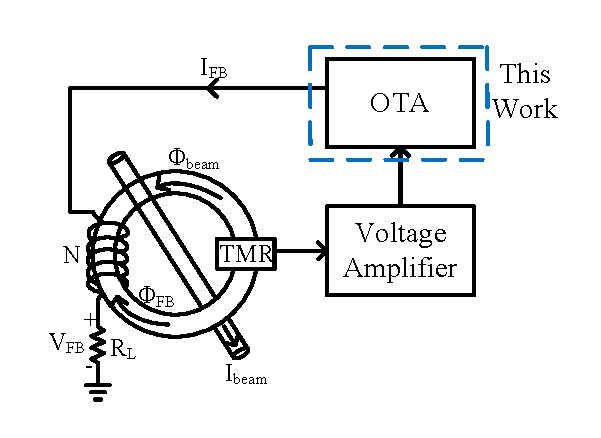
\includegraphics[scale=1]{Figures/System_Level/HRDCCT.pdf}
\caption{Closed Loop Novel-DC Current Transformer \cite{hrdcct}}
\label{fig:HRDCCT}
\end{figure}

\vfill
\clearpage

\section{Specification}
As the transconductance amplfier will be a part of the NDCCT, the specifications of the design were obtained from the commercial OTAs OPA860 and OPA861, which were simulated as on a PCB with a power supply of 5V and -5V as part of the N-DCCT in a closed loop. Since the OTA is being targetted for multiple applications - a closed loop DCCT and also for an Analog to Digial Converter (ADC), it is important to make the design programmable. The specifications are tabulated in detail in Table.\ref{tab:Specs}.

\begin{table} [H]
\centering
\begin{tabular}{@{}cc@{}}
\toprule
Parameter						& Value/Specification		\\ \midrule
Circuit Design					& Programmable via I/V/external R or C			\\
Transconductance Gain(Gm)		& 75 .. 140 mA/V			\\
Linear Input Voltage Range		& $\pm$200 mV				\\
Output Current Range			& $\pm$15 mA .. $\pm$30 mA	\\
Bandwidth						& 10 MHz					\\
Slew Rate						& $\pm$900 V/$\mu$s			\\
Rise/Fall time					& 4.4 ns					\\
Input Referred Noise			& 3 nV/$\sqrt{Hz}$ @few KHz	\\
Input Impedance					& 0.5 M$\Omega$				\\
Output Impedance				& 55 K$\Omega$				\\
HD2								& Less than -75 dBc			\\
HD3								& Less than -80 dBc			\\
Open Loop Voltage Gain			& Not less than+5 V/V		\\
PSRR							& $\pm$20 $\mu$A/V			\\
\bottomrule
\end{tabular}
\caption{Specifications of the Design}
\label{tab:Specs}
\end{table}

Remarks:
\begin{itemize}
\item Supply Voltage: 5V
\item Max Load Resistance: 1k$\Omega$
\item Technology to be used: XT018 from XFAB
\end{itemize}

\vfill
\clearpage

\section{Technology}

The technology used for designing the building blocks of the system is the XT018 technology. The XT018 series is XFAB's 0.18-micron Module High-voltage SOI CMOS Technology. It combines the benefits of SOI wafers with Deep Trench Isolation and those of a State of the art six metal layers 0.18-micron process\cite{xt018}. The technology related component names used as part of the circuit design are as tabulated in Table.\ref{tab:Components}.

\begin{table} [H]
\centering
\begin{tabular}{@{}ccc@{}}
\toprule
Component	& Name		& Description			\\ \midrule
PMOS		& pe5		& 5V PMOS				\\
NMOS		& ne5		& 5V NMOS				\\
Resistor	& rmtp		& Top Metal Resistor	\\
Capacitor	& cmm4t		& Single MIM Capacitor	\\
\bottomrule
\end{tabular}
\caption{Components used as part of XT018 technology}
\label{tab:Components}
\end{table}

Silicon on insulator (SOI) technology refers to the use of a layered silicon-insulator-silicon substrate in place of conventional silicon substrates in semiconductor manufacturing \cite{soi_tech}, especially microelectronics, to reduce parasitic device capacitance, thereby improving performance. The result is up to 30 percent lower power consumption, 20 percent higher poerformance and 15 percent higher density than the traditional bulk CMOS at the same feature size. SOI-based devices differ from conventional silicon-built devices in that the silicon junction is above an electrical insulator, typically silicon dioxide or sapphire. SOI inherently eliminates latchup \cite{soi_ease}, which can occur in CMOS devices due to parasitic conditions in which at least one transistor acts as a Silicon controlled rectifier (SCR). And since XT018 is an SOI technology, it is chosen to design the amplifier.

Radiation hardening is the act of making electronic components and systems resistant to damage or malfunctions caused by ionizing radiation (particle radiation and high-energy electromagnetic radiation), such as those encountered in outer space and high-altitude flight, around nuclear reactors and particle accelerators, or during nuclear accidents or nuclear warfare \cite{radhard}. Most semiconductor electronic components are susceptible to radiation damage; radiation-hardened components are based on their non-hardened equivalents, with some design and manufacturing variations that reduce the susceptibility to radiation damage \cite{radhard_effects}. 

\chapter{Theory}
\section{The Operational Transconductance Amplifier}
The operational transconductance amplifier (OTA) is basically an op-amp without an output buffer \cite{baker_book}. An OTA can be defined as an amplifier where all the nodes are low impedance except the input and output nodes. A schematic symbol of an OTA is shown in Figure.\ref{fig:OTA_symbol}. OTAs are generally programmable - usually through the bias current that is provided to the differential amplifier. In the symbol, a bias voltage is being used as a programmable input. This bias voltage in turn controls the bias current of the amplifier.

\begin{figure} [H]
\centering
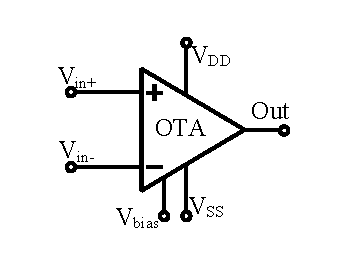
\includegraphics[scale=1]{Figures/System_Level/OTA_Symbol.pdf}
\caption{Symbol of an OTA}
\label{fig:OTA_symbol}
\end{figure}

\subsection{Conventional Current Mirror OTA}
The schematic of a conventional current mirror based OTA is as shown in Figure.\ref{fig:OTA_Schematic_Ibias}. The OTA employs a differential input pair in conjunction with three current mirrors. The differential input pair comprises of transistors $M_1$ and $M_2$. The differential pair is biased by the current mirror formed by $M_{nB1}$ and $M_{nB2}$. PMOS current mirrors formed by $M_3$, $M_5$ and $M_4$, $M_6$ reflect currents generated in the differential pair on to the output shell. The current generated by the mirror formed by $M_3$ and $M_5$ is reflected to the output via the NMOS current mirror formed by $M_7$ and $M_8$. The current mirror gain factor is K. Increase in K will increase the slew rate and gain bandwidth along with the output current of the conventional OTA at the cost of increased area, static power dissipation and a decrease in phase margin \cite{lcmfb_ota}.

\begin{figure} [H]
\centering
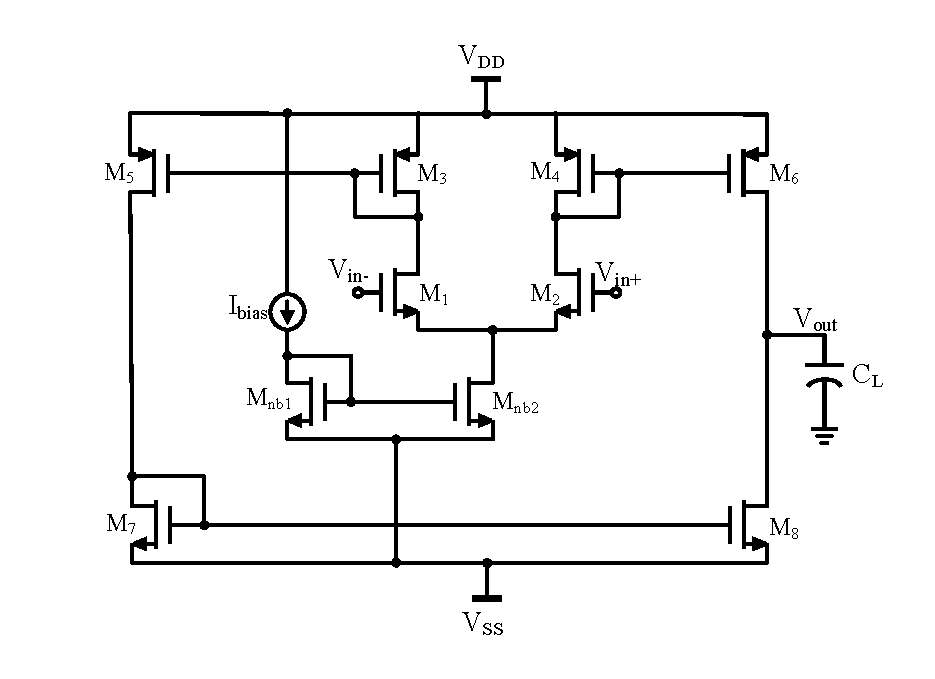
\includegraphics[scale=1]{Figures/Schematics/OTA_NMOS.pdf}
\caption{Schematic of a Conventional Current Mirror OTA}
\label{fig:OTA_Schematic_Ibias}
\end{figure}

Common mode signals are ideally rejected. i.e., when $V_{in+} = V_{in-}$, $I_{out}$ = 0. A differential input signal will generate an output current proportional to the applied differential voltage based on the transconductance of the differential pair. And that is why OTA is known as Voltage controlled Current Source. Although the output stage is push-pull structure, the conventional OTA is only capable for producing an output current with a maximum amplitude equal to the bias current in the output shell, provided the current mirror gain is unity, i.e., K=1. For this reason, conventional OTA is referred to as a Class A amplifier. 

The conventional OTA does not employ an output buffer and hence is only capable of driving capacitive loads and the capacitive load consumes all the current generated in the circuit. The gain of the OTA ($G_mR_o$) is dependent on the large output resistance of the output shell of the OTA formed by the transistors $M_3$ to $M_8$. The output resistance is reduced to $G_mR_o//R_L \approx G_mR_L$ if a parallel resistive load $R_L$ is applied.

Let us consider a hypothetical scenario that we do not need a resistive load to be driven as part of the system. In other words, we have a capacitive load as part of the specification. An advantage of this would be the fact that the need of an output buffer is eliminated and thereby the static power dissipation and the area occupied is reduced. But on the downside, the  amplifier behaviour for the output current would be like that of a band pass filter. So this scenario will not be useful as the specification demands a bandwidth of 10MHz. So a capacitive load will limit the output current only to a certain band of frequencies and hence it will not make sense to just use a one stage design. This gives rise to design an output buffer for the OTA.

An output buffer can either be a voltage buffer or a current buffer depending on how the OTA is designed. A current buffer, for example, is used to hold the output current of the OTA at the output of the buffer. So any amplification needed for this current would in turn give rise to the need of another stage, making the design complicated. In this case usually a current feedback amplifier is designed which theoretically has a low input impedance at its non-inverting terminal and a high input impedance at its inverting terminal. So the OTA output would directly be connected to this non-inverting terminal and with the use of internal buffers, the output current follows the input current.

In this work, however, a voltage buffer amplifier is designed. Therefore, the OTA is used as a programmable block to control the output voltage rather than the output current.

\subsection{Other Topologies}
The Conventional OTA considered in the previous section is a Class A type of amplifier. These amplifiers can produce output currents that are equal to the bias currents for a unity current mirror gain. Need for high speed and high current with low power dissipation gave rise to research in Class AB Amplifiers. There are many topologies of the Class AB type OTAs that are classified based on their structure as:
\begin{itemize}
\item Folded Cascode OTA \cite{folded_cascode}
\item Telescopic OTA \cite{telescopic}
\item Local Common Mode Feedback OTA \cite{lcmfb_ota}
\item Cascode Voltage Flipped Follower based OTA \cite{super_class_ab}
\end{itemize}

One of the figures of merit to compare these OTAs is the Current Enhancement factor (CE). $CE = I_{out-max}/2I_{bias}$. Class A amplifiers typically have a CE of 1. Class AB OTAs have a high CE value \cite{pourashraf2017high}. A family of OTA denoted as $Super Class-AB$ OTAs have remarkably large CE values. Typical value of CE ranges from 100 to 500 depending on the implementation of the Class-AB differential pair and the output branches. Cascode Voltage Flipped Follower based OTA is one such example of a Super Class-AB OTA. These OTAs have the largest reported CE in literature. Some of the other OTA designs considered are explained in the next chapter.

\vfill
\clearpage

\section{The Opeartional Amplifier}
The operational amplifier (OP AMP) is a fundamental building block in analog integrated circuit design. A typical symbol of an OP AMP is as shown in Figure.\ref{fig:OPAMP_symbol}. It consists of differential input terminals - inverting ($V_{in-}$) and non-inverting ($V_{in+}$), a positive supply pin ($V_{DD}$) and a negative/ground supply pin ($V_{SS}$) and the output terminal ($V_{out}$). Simple OP AMPs are generally used as summing amplifier, differentiator, integrator, transimpedance amplfier, and so on. OP AMPs with vastly different levels of complexity are used to realize functions ranging from dc bias generation to high-speed amplification or filtering.

\begin{figure} [H]
\centering
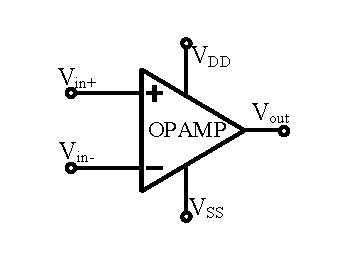
\includegraphics[scale=1]{Figures/System_Level/OPAMP_Symbol.pdf}
\caption{Symbol of an OP AMP}
\label{fig:OPAMP_symbol}
\end{figure}

OP AMPs are voltage controlled voltage sources, much to the contrary of OTAs, which are voltage controlled current sources. Design of an OP AMP consists of determining the specifications, selecting the device sizes and biasing conditions, compensating the op-amp for stability, simulating and characterizing the open loop gain, the input common mode range, common mode rejection ratio, power supply rejection ratio, output votlage range, current sourcing/sinking capability and power dissipation \cite{razavi_book}.OP AMPs are used as voltage buffers whenever there is a need to drive resistive loads or a combination of capacitive load and a resistive load.

\subsection{Miller Compensation OP AMP}
The schematic of the a two-stage Miller compensation OP AMP is as shown in Figure.\ref{fig:OPAMP_Schematic_Ibias}. First stage of the OP AMP is the differential amplfier formed by the transistors $M_1-M_5$ and $M_8$. The second stage of the OP AMP is the common source amplifier formed by the transistors $M_6$ and $M_7$. Compensation Capacitor or Miller Capacitor denoted by $C_C$ is used for the splitting of the poles of the two stages thereby providing stability and also controlling the bandwidth and the slew rate. 
\begin{figure} [H]
\centering
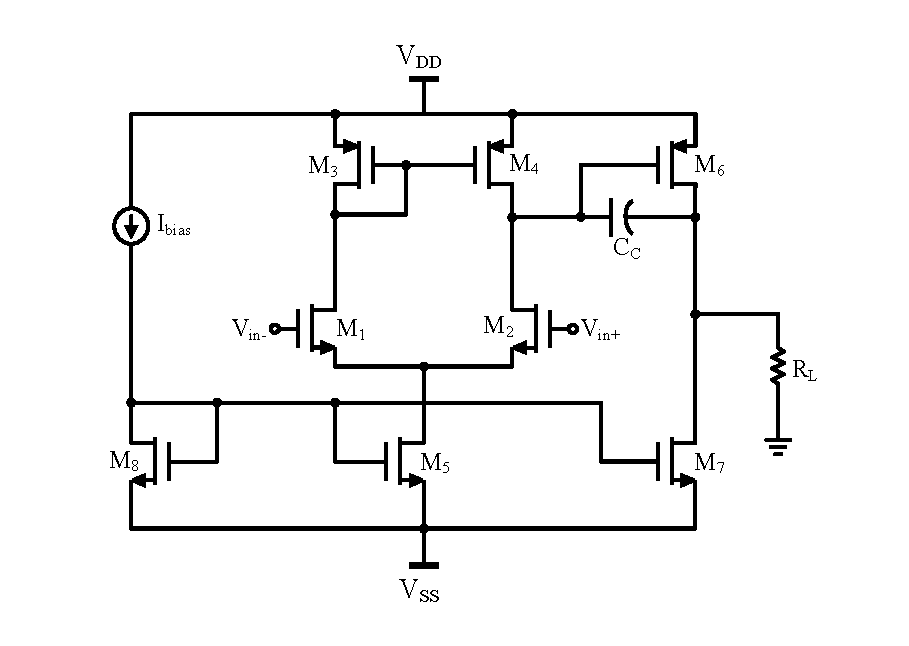
\includegraphics[scale=1]{Figures/Schematics/OPAMP_Ibias.pdf}
\caption{Schematic of a Two-stage Miller Compensation OP AMP}
\label{fig:OPAMP_Schematic_Ibias}
\end{figure}
The biasing to the differential input pair is provided by the current mirror formed by $M_5$ and $M_8$. The selection of the bias current, $I_{bias}$ is determined by gain, ICMR, CMRR, power dissipation, noise, slew rate and matching considerations. If slew-rate is of concern, a cross-coupled differential amplifier should be considered for the first stage. The second stage common source amplifier is used to provide an additional gain to the overall OP AMP since the gain provided by the differential pair is usually not large enough. It is known that OP AMPs have infinitely large open loop gain. This second stage also provided a current boosting since $M_7$ forms a current mirror with $M_8$ and the dimensions of $M_7$ are usually larger than $M_8$, thereby setting the current at the output of the OP AMP. The best use of these OP AMPs are made as part of voltage buffers. i.e., the OP AMP is connected in a unity gain configuration by providing a direct feedback from the output terminal to the non-inverting terminal.
\vfill
\clearpage
\section{The Gm/Id Methodology}

Good analog design is an art, not a science. Best works are still done on napkins and not on EDA tools, i.e., using Hand Calculations. However in recent times, in most cases at least, the equations which were once valid have become inadequate. The ability of these equations are limited to only certain cases \cite{gmid_vs_sqlaw}. The famous equation for $I_{ds}$ is naturally the first thing that comes to mind when we hear "Square Law", which is given by 
$$I_{ds} = \frac{\mu \cdot C_{ox}\cdot W}{2\cdot L}.(V_{gs}-V_{th})^2$$

The square law becomes linear in short-channel limit \cite{silveira1996g} and thus they are suitable only for long channel MOSFETs. The block diagram in Figure.\ref{fig:Square_Law} \cite{boris2017systematic} indicates the failure in Square law, especially in deep submicron technologies.

\begin{figure} [H]
\centering
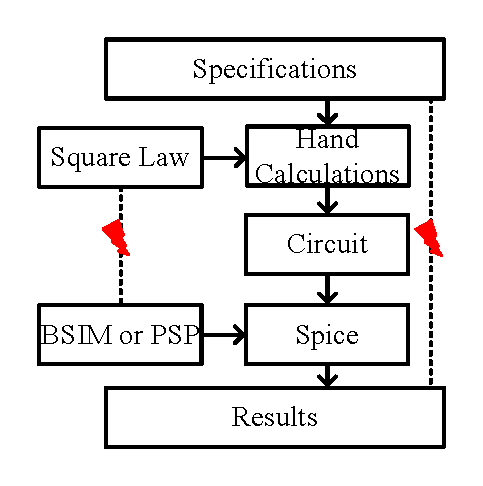
\includegraphics[scale=1]{Figures/Misc/PDFs/Square_Law.pdf}
\caption{Square Law Methodology}
\label{fig:Square_Law}
\end{figure}

The ratio W/L is directly proportional to the the transconductance($g_m$) and inversely proportional to the overdrive voltage. With $g_m$ fixed, a smaller overdrive voltage translates to a wider MOSFET and thus a large $C_{gs}$. Therefore, the overdrive voltage is not a good design parameter. The values obtained from hand calculations for short channel MOSFETs are far away from accuracy according to the requirements and thus there will be a huge gap in the spice simulation results and the specifications. The reason why this methodology has still not been a disaster is that fact that it over-predicts the $V_{dsat}$, but keeps the transistors in saturation. Micropower design techniques, on the other hand, exploit weak inversion models.

The $G_m$/$I_D$ methodology on the other hand, is fundamentally more practical. It is based on a unified synthesis methodology in all the regions of operation of a MOSFET. This methodology uses pre-computed spice data in hand calculation, thereby providing accurate results. The diagram in Figure.\ref{fig:GmID} shows that this methodology uses design tables which are pre-computed and using those tables, the hand calculations are made, which are rather simple and straight forward. 

\begin{figure} [H]
\centering
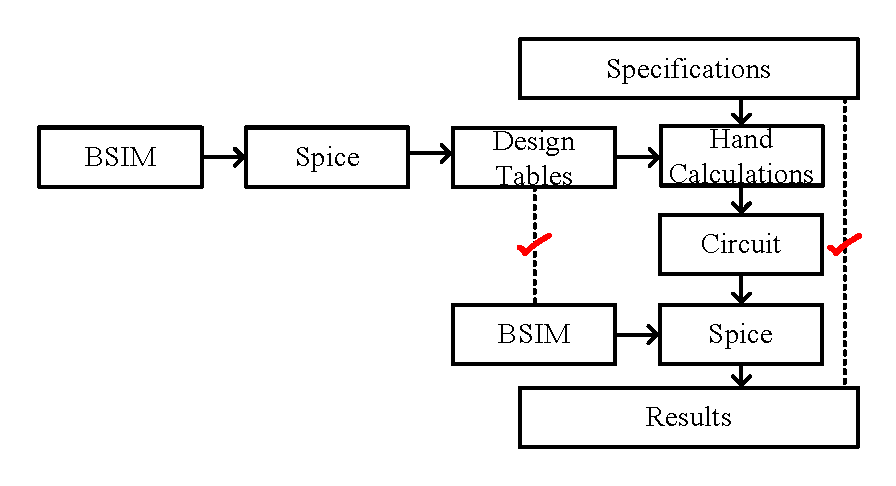
\includegraphics[scale=1]{Figures/Misc/PDFs/GmID.pdf}
\caption{Gm/ID Methodology}
\label{fig:GmID}
\end{figure}
To obtain the design tables, we need to look at a transistor in terms of width-independent figures of merit that are linked to the design specification. The design trade-offs have to be considered in terms of MOSFET's inversion level by using $G_m$/$I_D$ as a proxy \cite{gmid_basic}. What we really need from a MOSFET is - Large $g_m$ without investing much current and without having large $C_{gs}$. To quantify how good of a job our transistor does, we can define certain "figures of merit". The figures of merit considered as part of this work for $G_m$/$I_D$ methodology are $G_m$/$I_D$, $f_T$(transit frequency), $G_m$/$G_{ds}$(intrinsic gain), $I_D$(drain current), $f_TG_m$/$I_D$ (design trade-off). The circuit in Figure.\ref{fig:GmID_Ckt} is used to simulate these figures of merit parameters that are necessary to make design decisions. The width of the transistor $M_0$ is set to 5$\mu$m and the length is kept as a variable. The value of $V_{ds}$ is set to a value that is half of the value of the power supply. As part of this work, the supply we use is +2.5V and -2.5V. So technically we have a voltage difference of 5V and therefore, the value of $V_{ds}$ is set to 2.5V. 
\begin{figure} [H]
\centering
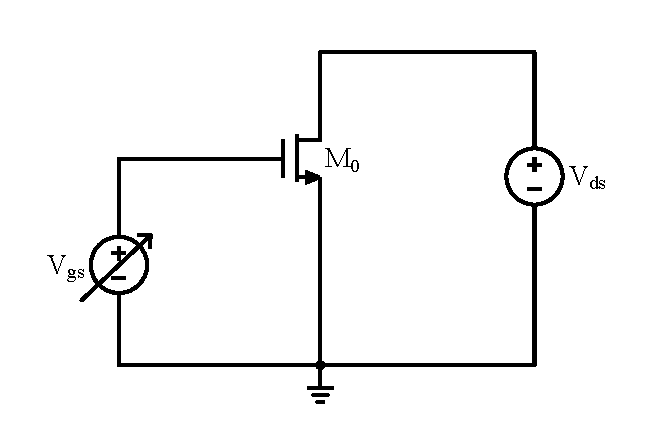
\includegraphics[scale=1]{Figures/Misc/PDFs/GmID_NMOS.pdf}
\caption{Setup for simulating GmID parameters}
\label{fig:GmID_Ckt}
\end{figure}

\begin{figure} [H]
\centering
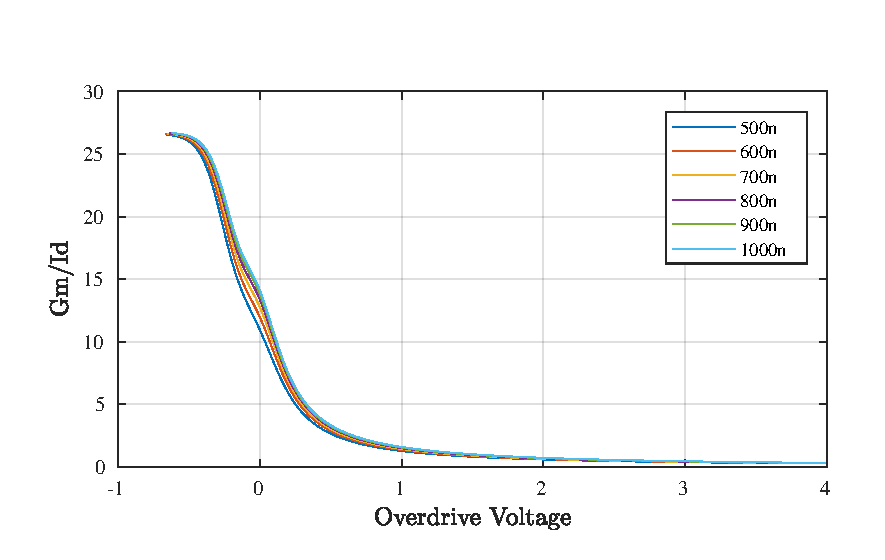
\includegraphics[scale=1]{Figures/Misc/PDFs/nmos_len_vovgmid.pdf}
\caption{$G_m$/$I_D$ vs $V_{ov}$}
\label{fig:vovgmid}
\end{figure}

The plot of $G_m$/$I_D$ versus the Overdrive voltage for different lengths is shown in Figure.\ref{fig:vovgmid}. The value of $G_m$/$I_D$ is very high when the overdrive voltage is less than zero, i.e., when the transistor is in weak inversion. The gain starts dropping with increase in overdrive voltage and it becomes close to zero and constant and theat is where the transistor goes into strong inversion. The response to variation in length is minimal for this parameter.

\begin{figure} [H]
\centering
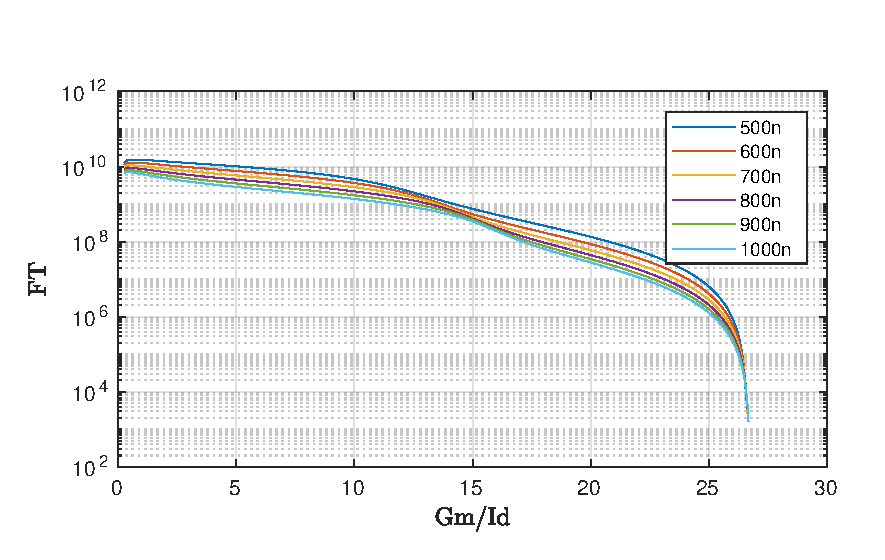
\includegraphics[scale=1]{Figures/Misc/PDFs/nmos_len_gmidft.pdf}
\caption{$f_T$ vs $G_m$/$I_D$}
\label{fig:gmidft}
\end{figure}

Transit frequency is defined as the ratio of the transconductance $G_m$ to its gate to source capacitance $C_{gs}$. The plot of transit frequency against $G_m$/$I_D$ for different lengths is as shown in Figure.\ref{fig:gmidft}. This figure of merit is used to indicate the speed of operation of the MOSFET. And from the plot, it can be seen that the speed is high when the value of $G_m$/$I_D$ is low. So this is quite the opposite to the gain parameter that was discussed with the previous plot. So here we have our first trade-off between high gain and high speed.

\begin{figure} [H]
\centering
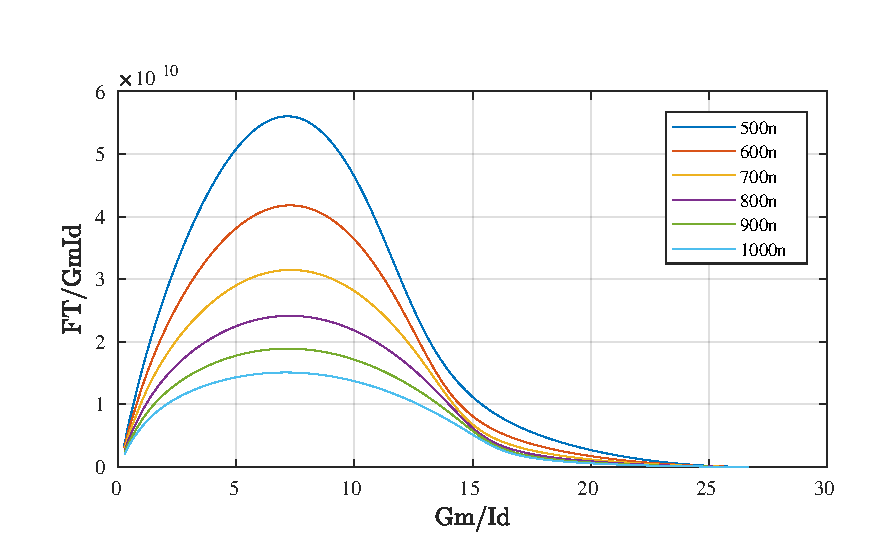
\includegraphics[scale=1]{Figures/Misc/PDFs/nmos_len_gmidftgmid.pdf}
\caption{$f_TG_m/I_D$ vs $G_m$/$I_D$}
\label{fig:gmidftgmid}
\end{figure}

To evaluate the trade-off mentioned above, the product of the two figures of merit are considered and then plotted against the $G_m$/$I_D$ parameter and is plotted as shown in Figure.\ref{fig:gmidftgmid}. This product is highest in moderate inversion. And this is called as the sweet spot and this provides the best possible trade-off between gain and speed. This is something that the mainstream methods like Square Law fail to provide because these methods generally assume strong inversion.

\begin{figure} [H]
\centering
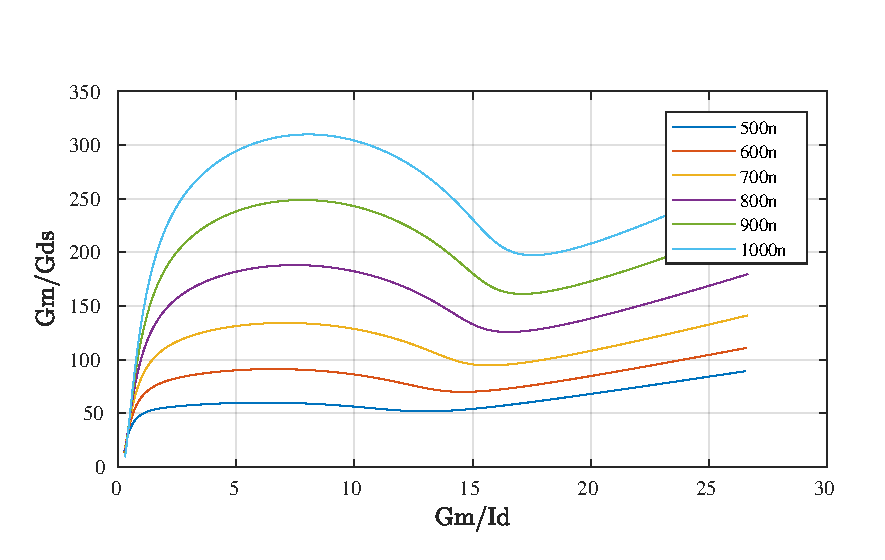
\includegraphics[scale=1]{Figures/Misc/PDFs/nmos_len_gmidgmgds.pdf}
\caption{$G_m/G_{ds}$ vs $G_m$/$I_D$}
\label{fig:gmidgmgds}
\end{figure}

The intrinsic gain $G_m/G_{ds}$ is plotted against $G_m$/$I_D$ as shown in Figure.\ref{fig:gmidgmgds}. This along with Figure.\ref{fig:gmidft} form a powerful tool in choosing the value of the channel length that meets the gain requirements. The plot in Figure.\ref{fig:vovgmid} did not show too much of a variation with respect to length. But using this plot it is easy to decide the channel length of the transistor. It is clear that the smallest channel length in moderate inversion provide the highest gain with a decent trade-off with respect to speed, i.e., transist frequency.

\begin{figure} [H]
\centering
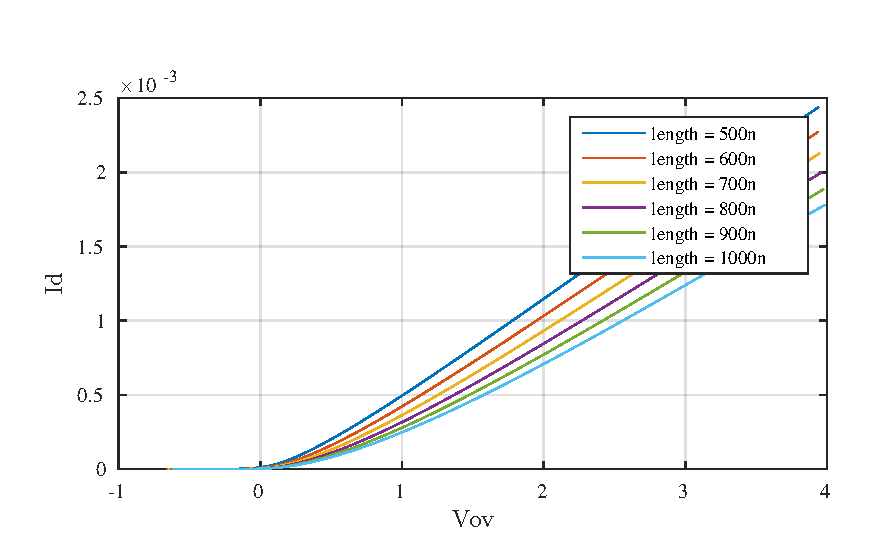
\includegraphics[scale=1]{Figures/Misc/PDFs/nmos_len_vovid.pdf}
\caption{$I_D$ vs $V_{ov}$}
\label{fig:vovid}
\end{figure}

The final plot is to choose the drain current for the overdrive voltage needed. It is as shown in Figure.\ref{fig:vovid}. Ultimately, it is the overdrive voltage that determines the region of operation of the transistor. So with the overdrive voltage known and the length of the transistor decided, the drain current can be easily chosen.

An important thing not to forget is that the figures of merit simulated and plotted are independent of variation in the width of the transistor. So once the other parameters are decided, the value of W can be chose using the Id/W plot. The steps involved in the general design flow of this methodology is summarized below.
\begin{itemize}
\item Determine $G_m$ from (design objectives)
\item Pick the channel length L
	\begin{itemize}
	\item Short channel $\rightarrow$ high $f_T$ (high speed)
	\item Long channel $\rightarrow$ high intrinsic gain
	\end{itemize}
\item Pick $G_m$/$I_D$ (or $f_T$)
	\begin{itemize}
	\item Large $G_m$/$I_D$ $\rightarrow$ low power, large signal swing
	\item Small $G_m$/$I_D$ $\rightarrow$ high $f_T$ (high speed)
	\end{itemize}
\item Determine $I_D$ (from $G_m$ and $G_m$/$I_D$)
\item Determine W (from $I_D$/W)
\end{itemize}

There are many other possibilities to design using this methodology and this depends on the specifications, constraints and objectives. However, as part of this thesis the steps mentioned above are followed and the plots discussed above are used to design the differential pair of transistors for all the stages of the system. And the other transistors' dimensions were finalized using simulations.

\chapter{Operational Transconductance Amplifier}

\section{Design and Implementaion}
OTAs are versatile building blocks that offer a wide bandwidth for many types of amplifiers. OTA can work in a voltage mode as well as a current mode. As part of this work, the OTA is used in voltage mode. Most circuits for the OTA of a given application consists of variation on a few basic types. And because OTAs have a wide range of applications, there are several different topologies that are useful for these applications. The typical topologies were studied as part of this thesis and an overview at a system level for each of them is provided in the subsequent sections.

\subsubsection{Commercial OTA}
OPA860 by Texas Instruments is one of the most popular commercial OTA in the market. The design document \cite{opa860} of OPA860 compares OTA to a 3 terminal transistor - a high impedance input(base), low impedance inout(emitter) and a current output(collector). OTA is therefore bipolar and self-biased. Being self-biased simplifies the design process and reduces component count. The overview of the OTA is as shown in Figure.\ref{fig:OPA}. The transconductance of the OTA can be adjusted using an external resistor, allowing bandwidth, quiscent current and gain trade-offs to be optimized. Reducing or increasing the size of the OTA controls the bandwidth, AC behavior and transconductance. With a fixed external resistor, the quiscent current increases with increase in temperature. The variation of the current with temperature holds the transconductance of the OTA relatively constant with temperature.

\begin{figure} [H]
\centering
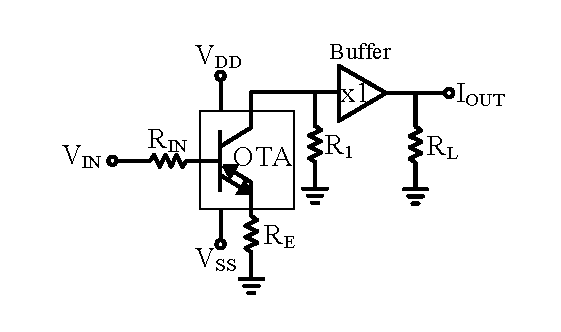
\includegraphics[scale=1]{Figures/Misc/PDFs/OPA.pdf}
\caption{Overview of Commercial OTA OPA860}
\label{fig:OPA}
\end{figure}

The commercial OTA in review, can operate in 2 modes - Voltage mode and Current mode. In voltage mode, it can operate in 3 states - common emitter, common base and common collector. In current mode, it is useful for analog communication such as current amplifier, current differentiator, current integrator and current summer. The output offset voltage is usually very close to zero for an OTA.

Having stated all these facts, this commercial OTA is an amplifier based on BJTs. Considering the high power dissipation and high input current noise of a BJT based amplifier, it is not suitable for our system. However, the concept of having an OTA and an output buffer \cite{lt1228} is something that can be pondered upon.

\subsubsection{Self-Cascode OTA}
An intruiging concept of Self-Cascode can be used to achieve very high gain for a low supply voltage. A high gain 2-stage self cascode OTA for a 1V supply was researched as part of \cite{scmos_ota}. A self-cascode MOSFET (SCMOS) has a similar geometrical structure to a regular MOSFET. But still, the transconductance, and the output resistance of an SCMOS are much better than its conventional counterpart. A regular channel requires a long channel for high gain and a short channel for high speed. With the same channel length of a regular MOS, an SCMOS will provide a much higher gain without compromising the speed. 
An SCMOS is formed where a regular MOSFET will be replaced by two transistors whose gates are tied together, as shown in Figure.\ref{fig:SCMOS}. The two transistors have same widths. The operating regions of $M_1$ and $M_2$ depend upon the common gate voltage of the SCMOS. If $V_g$ is greater than $V_{th}$ of both the MOSFETs, then $M_1$ and $M_2$ operate in linear and saturation region respectively. With a bulk bias, the threshold voltage of the drain transistor ($M_2$) decreases. This increases the $V_{ds}$ of $M_1$, resulting in moving of its operating point from linear to edge of saturation, i.e., moderate inversion. And this is where the gain is high. Suppose both transistors are operating in saturation, the maximum output resistance can be achived but the voltage swing is considerably reduced.

\begin{figure} [H]
\centering
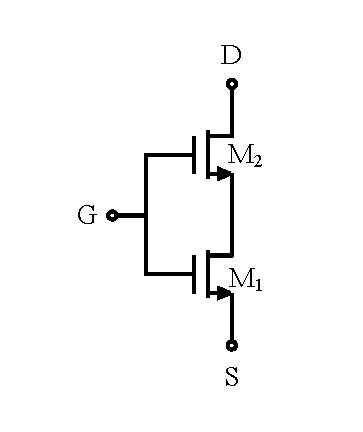
\includegraphics[scale=1]{Figures/Misc/PDFs/SCMOS.pdf}
\caption{Schematic of a Self-Cascode MOSFET}
\label{fig:SCMOS}
\end{figure}

In the context of an OTA, consider a conventional OTA with their regular MOSFETs replaced by SCMOS. To improve the gain of the OTA, positive feedback is created by cross coupling the bulk terminals of the input stage load transistors. Smaller channel length CMOS requires scaling down of power supply to maintain reliability of the circuit. A dual function gate MOSFET with a focus on increasing output resistance and transconductance is equivalent to a self cascode structure. A floating gate MOSFET is another alternative to the conventional techniques used to enhance DC gain. But, both these techniques require complicated fabrication steps. On the other hand, a current shunt technique can be applied to a self-cascode OTA to increase its gain. But this has reduced phase margin and requires compensation circuit even for a single stage.

A self-cascode OTA is very hekpful in achieving a high gain for low power supplies. But give the nature of our system, and the fact that the OTA to be designed as part of this system is to be an open loop amplifier, a very high gain is something that is suitable for the system in order to avoid saturation at the output as the headroom for output transistors would be very less. Another possible drawback is that the self-cascode OTA exhibits a slew rate that is lesser than the conventional OTA because the output current is low. But in case our system had to work in a closed loop, then this concept of self-cascode would have been a better fit.

\subsubsection{2-stage Feed Forward Miller Compensation OTA}

The system level diagram of a feed-forward Miller compensated OTA is shown in Figure.\ref{fig:FFMCO}. The $g_{m1}$ and $g_{m2}$ are input and output stage of the OTA and $g_{mf}$ is the feed-forward path from input to output node. The implementation is based on feed-forward technique proposed in \cite{feed_fwd_miller}. There is no concept of pole spiltting. The location of poles is mainly dependent on the internal node impedance and parasitic capacitance. It is difficult to estimate the parasitic capacitances and it makes the design complex. Therefore the dominant and non-dominant pole locations will change when the OTA is configured in a closed loop. But using Miller compensation, the poles can be placed at desired locations.

\begin{figure} [H]
\centering
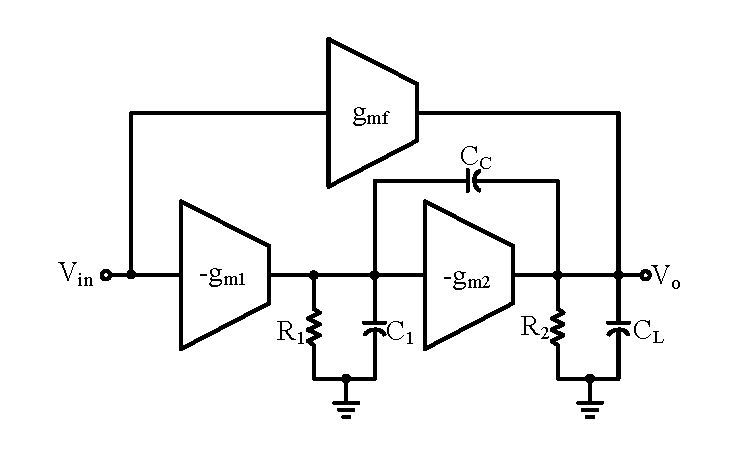
\includegraphics[scale=1]{Figures/Misc/PDFs/FFMCO.pdf}
\caption{Block Diagram of Feed Forward Miller Compensation OTA}
\label{fig:FFMCO}
\end{figure}

This topology of OTA is considered to consume less power than the conventional Miller compensation OTA. Feed forward compensation technique gives wider bandwidth as compared to the Miller OTA and is much more easier to stabilize.  However the overall bandwidth is lesser than what a conventional current mirror based OTA can provide. Current replicating branch with scaled down transistors can be used to implement a push-pull output stage that gives the maximum output current several times higher than that of bias current. Cascoding and gain boosting are conventional techniques for gain enhancement. But for low voltage designs, these techniques are not suitable due to limited head room. Cascading multiple gain stages is another alternative for the gain enhancement. But in a closed loop, the amplifier becomes unstable due to high impedance nodes at each stage, which produces negative phase shift and degrades the overall phase margin. To overcome this, the multi-stage amplifier needs a compensation circuit to achieve a minimum phase margin for stability.

The results of this topology were interesting and encouraging. But that fact that needs multiple stages and compensation circuitry just for a OTA without a buffer, makes it complex in spite of the encouraging remedies. So weighing the pros and cons of the topology and comparing it with other OTAs in review, this topology was deemed to be a bit too much for our requirements and question of feasibility comes into picture.

\subsubsection{A robust Feed Forward scheme without Miller capacitance}

This scheme uses a positive phase shift of left hand plane (LHP) zeros caused by the feedforward path to cancel the negative phase shift of poles to attain good phase margin. The two-stage path increases the low frequency gain further  while the feed forward single stage amplifier makes the circuit faster. The amplifier bandwidth is not compromised by the absence of the traditional pole-splitting effect of Miller compensation capacitor, resulting in a high gain wide-band amplifier \cite{robust_feed_fwd}.

\begin{figure} [H]
\centering
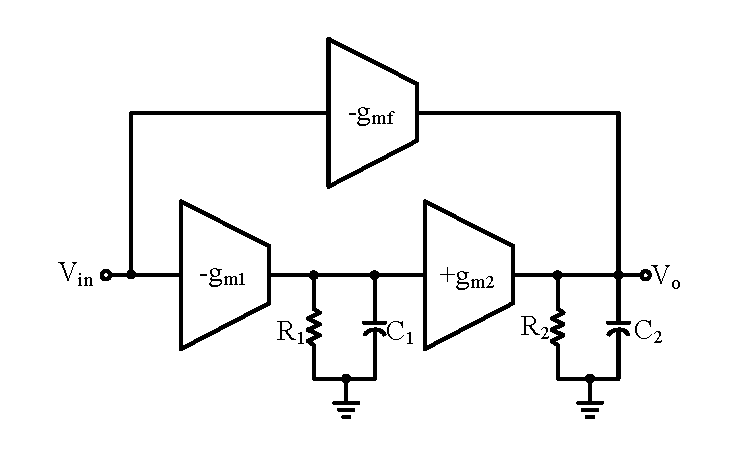
\includegraphics[scale=1]{Figures/Misc/PDFs/FFNMCO.pdf}
\caption{Block Diagram of Feed Forward OTA without Miller Capacitor}
\label{fig:FFMNCO}
\end{figure}

Amplifiers with high-gain generally use multi-stage designs. And trasistors with long channgel length are chosen and biased at low current levels. Amplifiers with high-bandwidth use single-stage designs with short channel length transistors biased at high current levels. In a Miller compensated amplifier, due to the Miller effect, the dominant pole is pushed towards lower frequencies, resulting in lower bandwidth. Along with this, the phase response is degraded with a RHP zero. A nulling resistor is used to cancel the effect of this RHP zero. The pole-zero pair is created at high frequencies to acoid the slow settling components associated with pole-zero cancellation at low frequencies. 

This scheme results in an amplifier with high gain and fast respsone. Bandwidth improvement is due to the fact that poles are not split. There could be substantial reduction in the area and power as there is no Miller compensation capacitor. As part of the circuit realization, the second andd feed-forward stage should not have any dominant pole before overal frequency for gain bandwidth. Pole-zero cancellation should occur at high frequencies for best settling time performance. The first stage in this scheme is usually designed to have a high gain and a small load capacitance. The second and feedforward stages should be optimized for high bandwidth and medium gain performance.

This topology offers several advantages over the other topologies reviewed during the design phase. Some aspects to be careful about are - the feed-forward stage has to be optimized to make sure the pole-zero cancellation occurs at high frequency otherwise there is a possibility of having an unstable system. Another drawback as in the previous case is the complexity of the circuit given that this scheme was initially intended to work for a single input design. Having two different pairs to transistors that need biasing at its gate terminals along with the complexity of the design, makes the programmability of the circuit a mystery. And since that is an integral part of our specification, this scheme might not be entirely suitable for our design despite offering more advantages than disadvantages.

\subsubsection{Super Class AB OTA}
\begin{figure} [H]
\centering
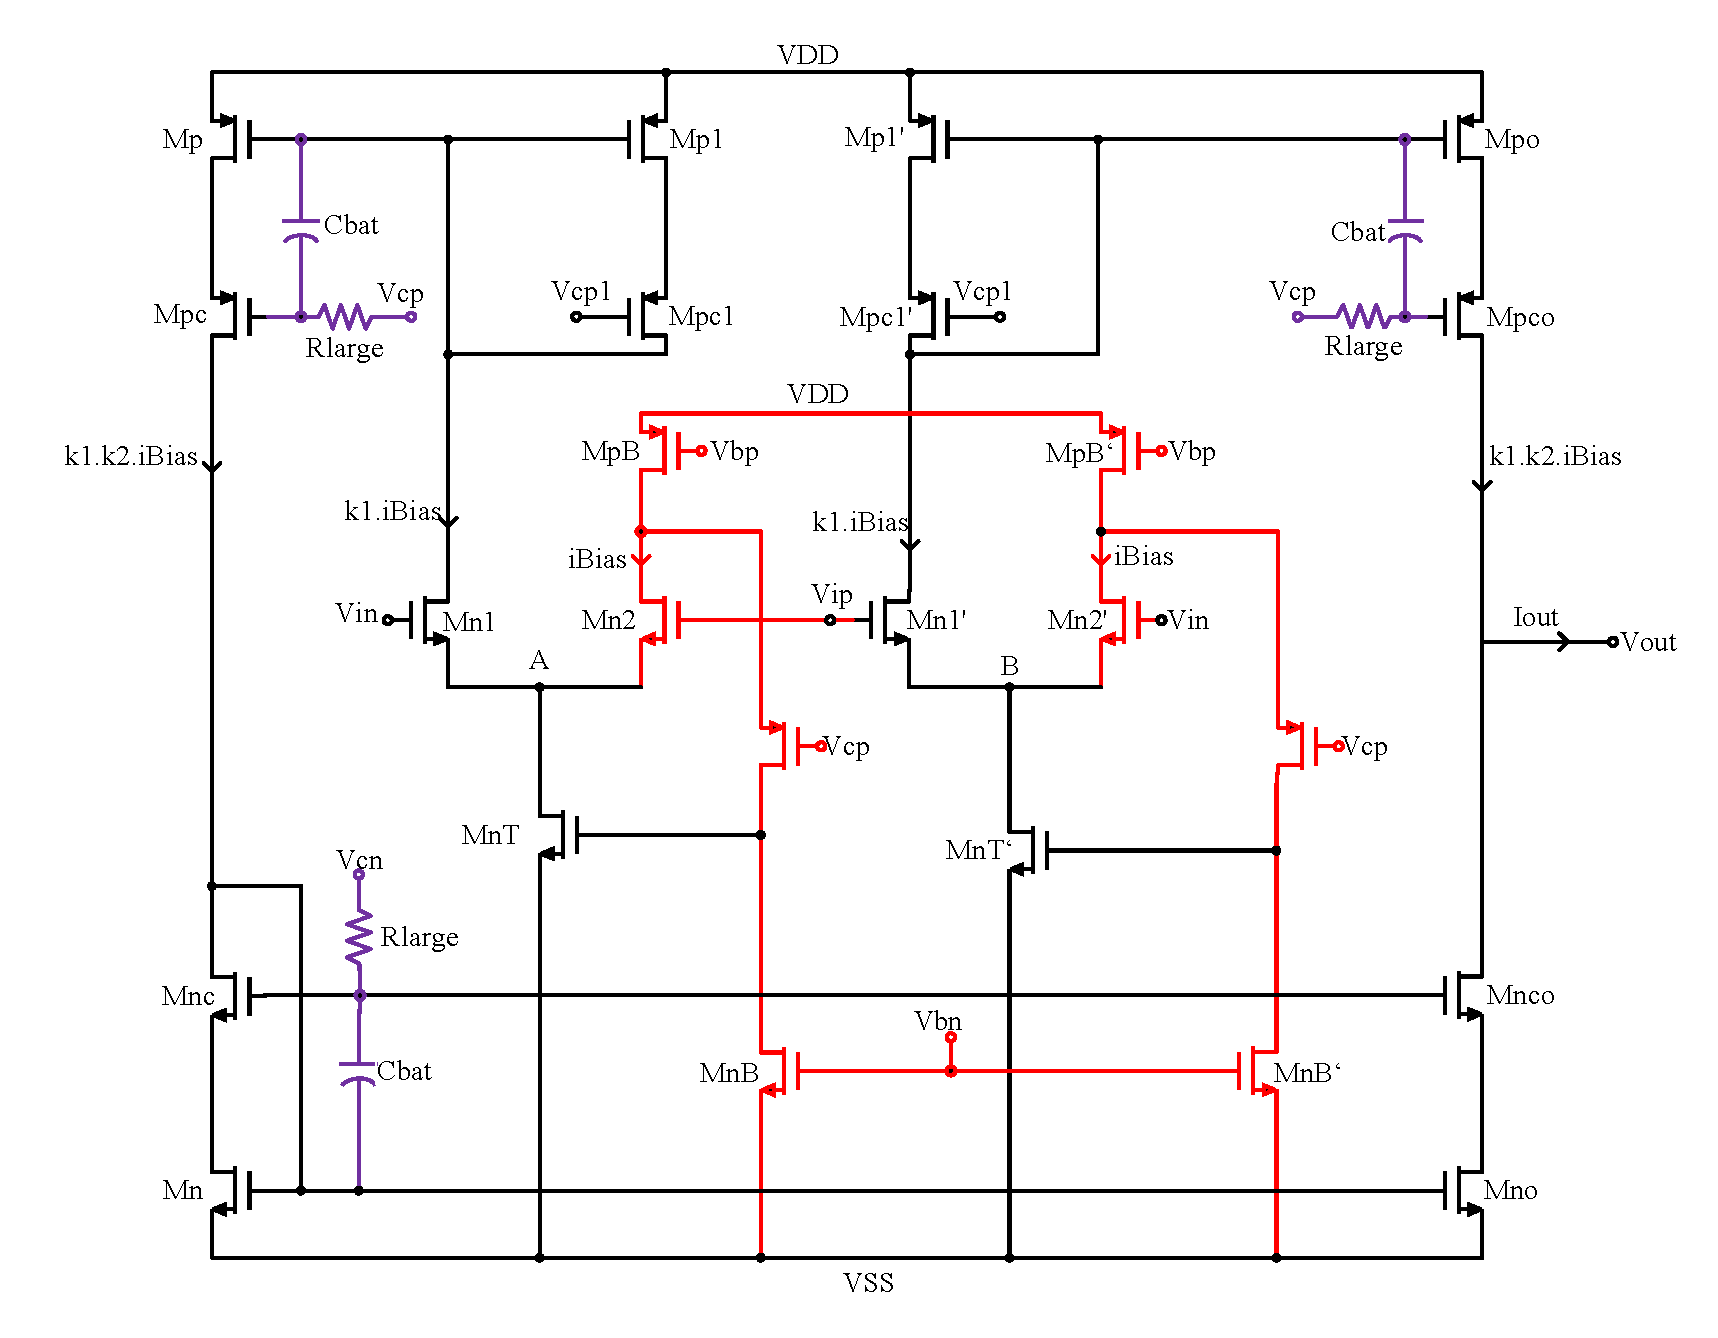
\includegraphics[scale=0.65]{Figures/Schematics/OTA_Class_AB.pdf}
\caption{Super Class-AB OTA with a Cascode Voltage Flipped Follower}
\label{fig:OTA_Class_AB}
\end{figure}

The schematic of a Super Class AB OTA based on a Cascode Voltage Flipped Follower is as shown in Figure.\ref{fig:OTA_Class_AB}. It uses a Class-AB differential pair to boost the bias current by a factor of $k_1$. Typical values of $k_1$ range from 30 to 60 depending on the implementation of the Class-AB differential pair and supply voltages. An additional current boosting by a factor of $k_2$ is obtained in the output branches. The typical values of $k_2$ range from 3-8. Using cascode transistors maximum output current and subsequently the CE values are reduced. But lack of cascode transistors results in very low open loop gain. Therefore, a simple power efficient technique is used that allows the use of cascode transistors in order to achieve even higher open loop gain and gain bandwidth by maintaining a large CE value. This is done with the help of dynamically biasing the cascode transistors using RC networks (indicated in purple in the figure) \cite{super_class_ab}. The capacitor $C_{bat}$ acts as a floating battery for dynamic operations that transfers variations in the gate voltages of mirror transistors to the gate of the cascode transistors. This increases the $V_{DS}$ of the mirror transistors allowing high output currents. Cascode Voltage Flipped Follower (indicated in red in the figure) is charaterized by high input swing and can operate over a wide range of supply voltages. It uses local shunt feedback to provide nodes A and B with very low impedance.

Taking into account the complexity, output current requirements and load requirements, this design will not be considered further as part of this research work. The reason being - a high current output of this Class AB OTA would give rise to another output buffer. And the capacitors needed to consume such a high current would be in the order of several pico Farads. Having such a big capacitor inside an IC is not recommended. Also, considering how complex CMOS Current Feedback Amplifiers are, it is wise to stick to a simpler design that does the same work but with some minor trade-offs.

\subsubsection{Conventional OTA}
Two separate designs - OTA with PMOS Differential pair and OTA with NMOS Differential pair were deisgned and simulated in Cadence to get a good understanding of the circuit parameters and how the differential pair impact them. 

Generally, amplifiers with PMOS transistors used as differential input offer high linearity, low flicker (1/f) noise. A possible reason to choose PMOS transistors as a differential pair comes from the necessity to reduce the influence of the substrate noise. The two transistors are in an N-well and the well is connected to the supply voltage that any substrate interference coupled via the parasitic capacitance to substrate is decoupled to the VDD line \cite{ota_hf}. P-channels typically have less flicker noise (1/f noise) caused by the carriers randomly enterring and leaving traps introduced by defects near the semiconductor surface. Since the majority charge carriers are holes in PMOS, there are less potential to be trapped in surface states.

Having stated all these facts, NMOS input transistors would be better in terms of transconductance gain, and hence thermal noise and the bandwidth of the amplifier. An important fact considered in the selection of the type of differential pair is that the OTA in this system is being used in an open loop. This means that the gain of the OTA has to be limited in order to avoid saturation at the crests and troughs at the output of the OTA.

PMOS transistors exhibit their low noise behaviour due to the fact that PMOS transistors are usually bigger (higher W/L ratio) than an NMOS pair. Since we need a small open loop gain, we cannot afford to have big transistors at the input that cause the output to saturate. Along with this, it was also seen that, the range of bias currents needed to obtain a similar range of voltage swing was much wider in case of PMOS than NMOS. Since this indirectly results in a high power dissipation in the 1st stage itself, it was concluded to use the NMOS based design as part of this Thesis work.
\vfill
\clearpage
\subsection{Schematic}

\begin{figure} [H]
\centering
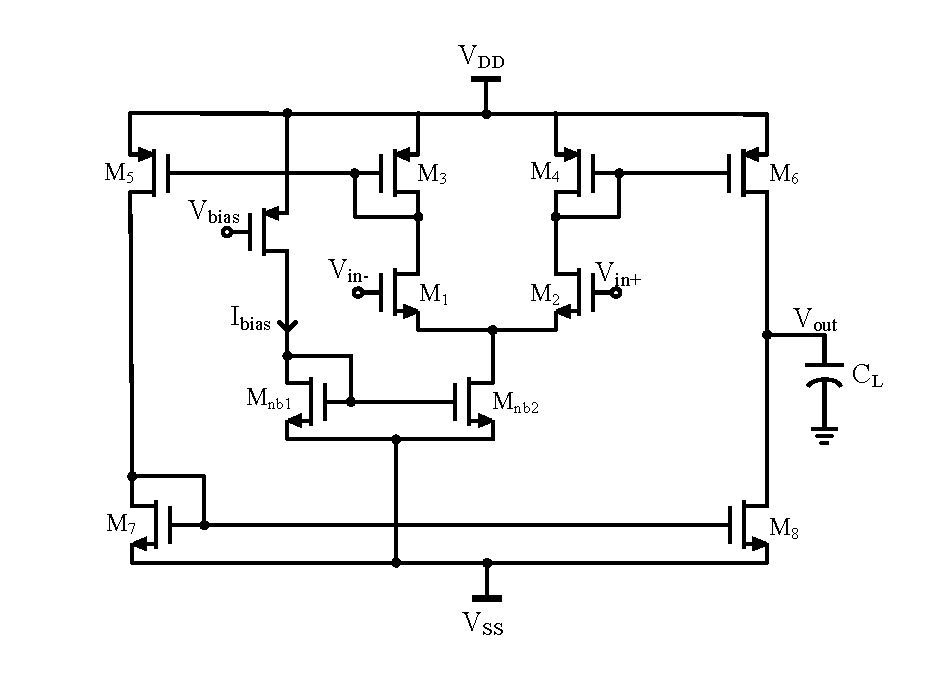
\includegraphics[scale=1]{Figures/Schematics/OTA_NMOS_Vbias.pdf}
\caption{Schematic of the OTA Designed}
\label{fig:OTA_Schematic}
\end{figure}

Figure.\ref{fig:OTA_Schematic} \cite{lcmfb_ota} shows the schematic of the OTA used as part of this Thesis. As mentioned above, the differential amplifier is formed by the NMOS pair $M_{1}$ and $M_{2}$ and dimensions of the differential pair was fixed using the figures of merit of the ${G_m/I_D}$ methodology. The bias current $I_{bias}$ to the differential pair is provided by the current mirror formed by $M_{nB1}$ and $M_{nB2}$ which is in turn controlled by the PMOS transistor $M_9$ whose gate voltage $V_{bias}$ is the programmable variable of the OTA and the entire system. This bias voltage is inversely proportional to the bias current flowing through each branch of the OTA.

\begin{table} [H]
\centering
\begin{tabular}{@{}cccc@{}}
\toprule
Transistor			& Width($\mu$m)		& Length(nm)		& Multiplier \\ \midrule
M1, M2				& 8					& 500n				& 5			\\
M3, M4				& 35				& 500n				& 1			\\
M5					& 28				& 500n				& 3			\\
M6					& 35				& 500n				& 3			\\
M7					& 35				& 500n				& 18		\\
M8					& 33				& 500n				& 18		\\
M9					& 10				& 500n				& 4			\\
MnB1, MnB2			& 20				& 500n				& 8			\\
\bottomrule
\end{tabular}
\caption{Dimensions of the Transistors of the designed OTA}
\label{tab:OTA_dimensions}
\end{table}
From the Table.\ref{tab:OTA_dimensions}, it can be seen that the current mirror gain for the current mirrors formed by $M_{3}$, $M_{5}$ and $M_{4}$, $M_{6}$ is 3. It can also be noted that the transistors $M_{5}$ and $M_{8}$ are not symmetric with respect to their counterparts. This is designed so to make sure the DC bias point at the output of the OTA is close to 0V, which is the mid point of $V_{DD}$ and $V_{SS}$. Changing the bias current of an amplifier, will automatically change the DC bias point at its output. Since we are using the OTA as a programmable block, it is important to have an output which is symmetric over 0. Even though it is not entirely possible, making these two transistors a little assymetric or uneven would close the gap between the bias points for highest and lowest bias currents. Initailly during the design phase, the load capacitance value was set at 1pF. Since it was necessary to have a second stage for the OTA, it only made sense to have a smaller capacitor as it would be going as part of the IC. Keeping that in mind and simulating the OTA with the OP AMP, the load capacitance is set at 50fF in order to achieve the required bandwidth and a stable enough system across various values of $V_{bias}$.

\section{Test Setup}
The test bench setup for the operation transconductance amplifier is as shown in Figure.\ref{fig:OTA_TB}. All the analyses are carried out under a standard temperature of $27^0C$, typical mean conditions for the NMOS transistors, PMOS transistors, capacitors and resistors unless explicitly mentioned otherwise. The $ocean$ script containing all the expressions to measure the various parameters of the OTA are attached in the Appendix. In the following subsections, the results of these parameters are discussed using DC Analysis, AC Analysis, Transient Analysis and Noise Analysis separately.

\subsection{DC Analysis}
The test bench in Figure.\ref{fig:OTA_TB}(a) and (b) are used to perform the DC analysis. The test bench in (a) is used to meausre the DC bias point at the output of the OTA. Since the programmable input indirectly controls the bias current, the DC bias at the output consequentially changes as the current flowing through the output branches is a function of a bias current due to the current mirror configuration between the adaptive load and the output shell. So for large bias currents, the DC bias point is a higher value and vice versa.
 
$V_{DD}$ = 2.5V; $V_{SS}$ = -2.5V; $V_{cm}$ = 1.95V; $V_{bias}$ = 150mV to 700mV;   $C_{L}$ = 50fF.

\begin{table} [H]
\centering
\begin{tabular}{@{}cccccccc@{}}
\toprule
Vbias (mV)					& 150		& 200			& 300			& 400			& 500			& 600			& 700 \\ \midrule
Output DC Bias (mV)			& 13.68		& -16.43		& -78.96		& -144.6		& -213.3		& -285.2		& -360.3 \\
\bottomrule
\end{tabular}
\caption{Output DC Bias Point of the OTA}
\label{tab:OTA_DC_Bias}
\end{table}

The output DC bias points for various values of $V_{bias}$ is tabulated in Table\ref{tab:OTA_DC_Bias}. The DC voltage at the output decreases with the increase in bias voltage or decrease in bias current. The test bench in (b) is used to check the offset voltage of the OTA. With a varying DC bias, there will be different offset voltage for each $V_{bias}$ which does not make sense since the offset voltage is usually a single value.

\subsection{AC Analysis}
The test bench in Figure.\ref{fig:OTA_TB}(a),(c),(d),(g) and (h) is used to analyse the small signal parameters of the OTA.

\begin{figure} [H]
\centering
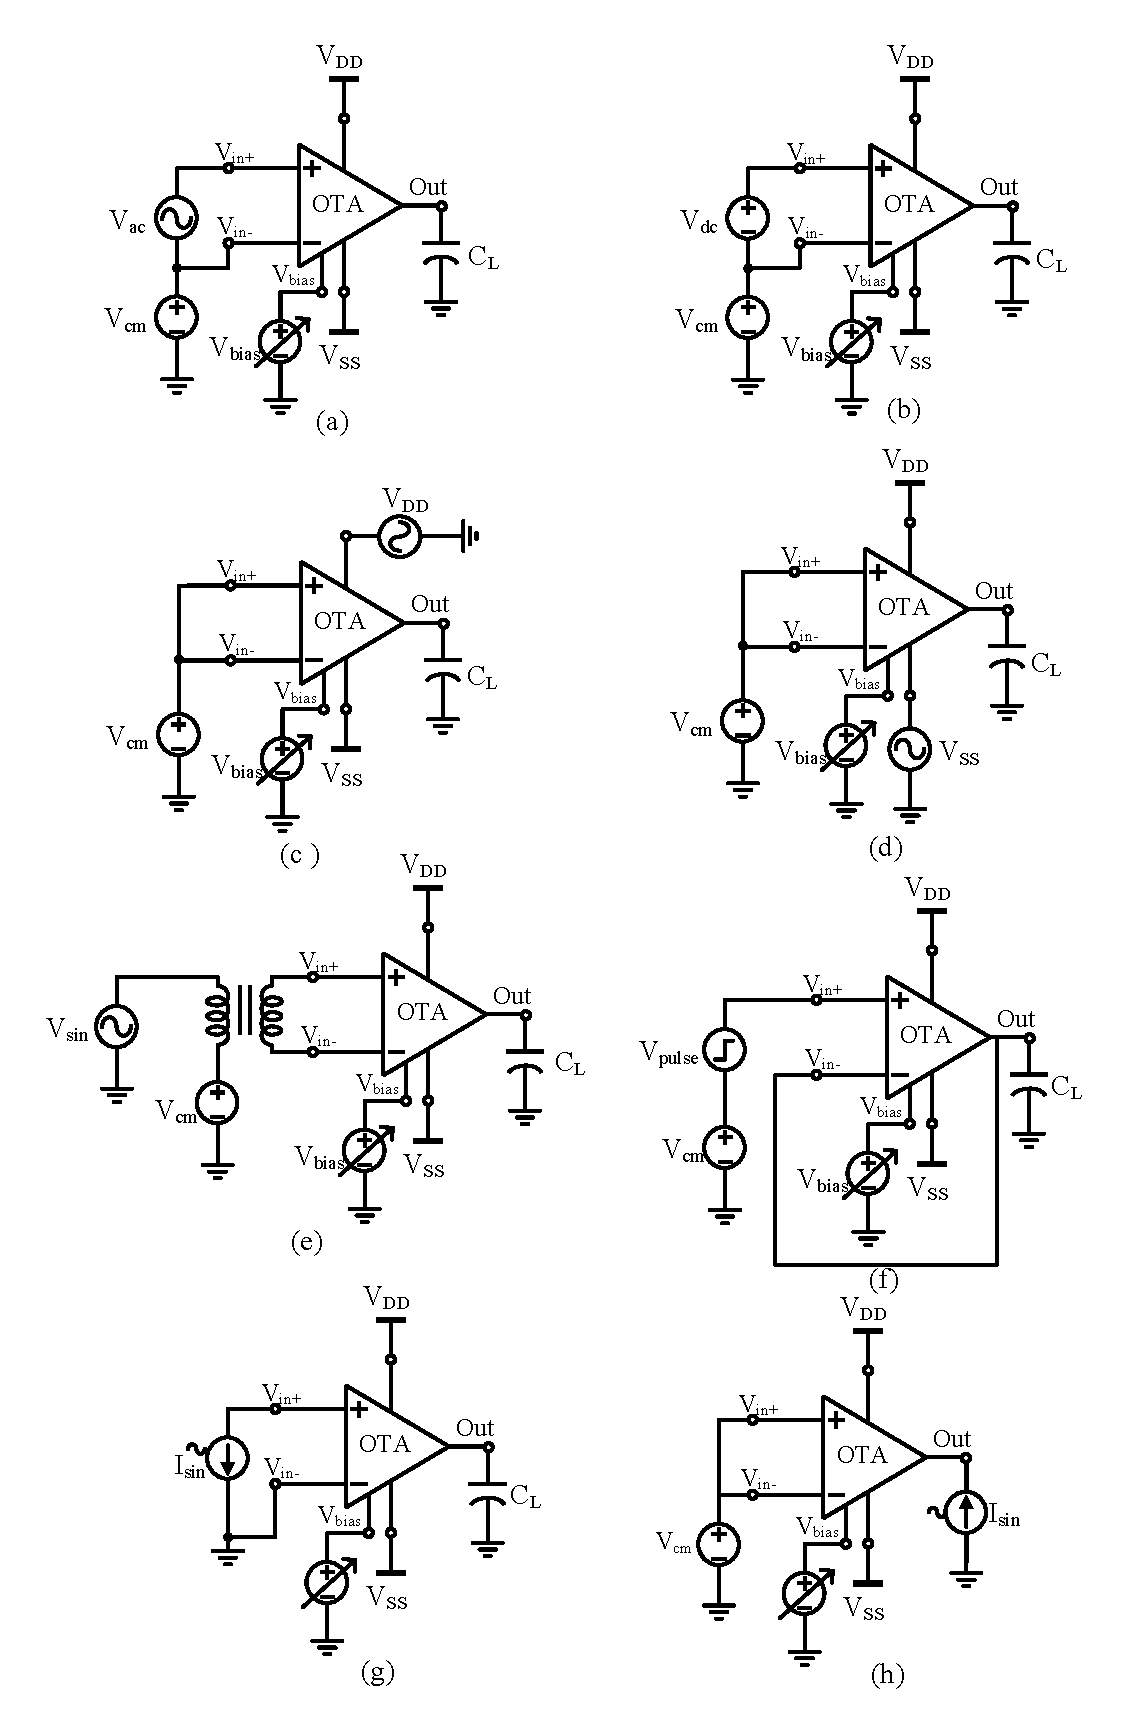
\includegraphics[scale=0.78]{Figures/Test_Benches/OTA_TB.pdf}
\caption{Test bench setup for OTA}
\label{fig:OTA_TB}
(a)Bias, Gain, Bandiwdth, Input Referred Noise; (b)Offset; (c)PSRR($V_{DD}$); (d)PSRR($V_{SS}$); (e)Transient - Sine; (f)Transient - Square; (g)Input Impedance; (h)Output Impedance
\end{figure}

\subsubsection{Gain, Bandwidth and Phase Margin}
Consider the Figure.\ref{fig:OTA_TB}(a) with the circuit condtions:

$V_{DD}$ = 2.5V; $V_{SS}$ = -2.5V; $V_{cm}$ = 1.95V; $V_{bias}$ = 150mV to 700mV;  $V_{ac}$ = 1V; $C_{L}$ = 50fF.
$$Gain in dB = 20 log_{10}\frac{V_{out}}{V_{in}}$$
Figure\ref{fig:OTA_Gain} shows the semilog plot of Gain for maximum and minimum $V_{bias}$. The plots for the other values of $V_{bias}$ are not shown here for simplicity.

\begin{figure} [H]
\centering
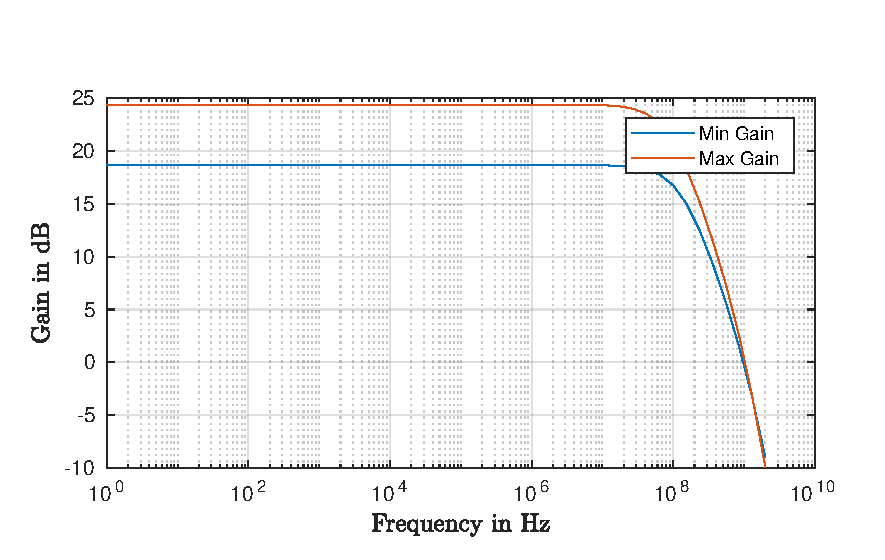
\includegraphics[scale=1]{Figures/Plots/OTA_Gain.pdf}
\caption{OTA Plot of Gain vs Frequency for different Vbias}
\label{fig:OTA_Gain}
\end{figure}

The variation of open loop gain of the OTA, its bandwidth and the phase margin with respect to $V_{bias}$ is tabulated in Table.\ref{tab:OTA_gain_bw_pm}. The bandwidth is kept at a high value in order to make sure that the dominant poles of the first and second stages are sufficiently far from each other so as to obtain a stable system for operation. The maximum open loop gain for this system is 23.7dB. Any value beyond this will cause the amplifier to saturate at the crests and troughs of the output voltage.

\begin{table} [H]
\centering
\begin{tabular}{@{}cccccccc@{}}
\toprule
Vbias (mV)					& 150		& 200		& 300		& 400		& 500		& 600		& 700 \\ \midrule
Open Loop Gain (dB)			& 18.64		& 19.46		& 20.9		& 22.05		& 22.96		& 23.7		& 24.35 \\
Phase Margin (degrees)		& 63.3		& 60.63		& 55.96		& 52.42		& 49.91		& 48.12		& 46.72 \\
Bandwidth (MHz)				& 135		& 130.7		& 122.2		& 113.7		& 105		& 96.63		& 89.19 \\
\bottomrule
\end{tabular}
\caption{Open Loop Gain, Phase Margin and Bandwidth of the OTA}
\label{tab:OTA_gain_bw_pm}
\end{table}

\begin{figure} [H]
\centering
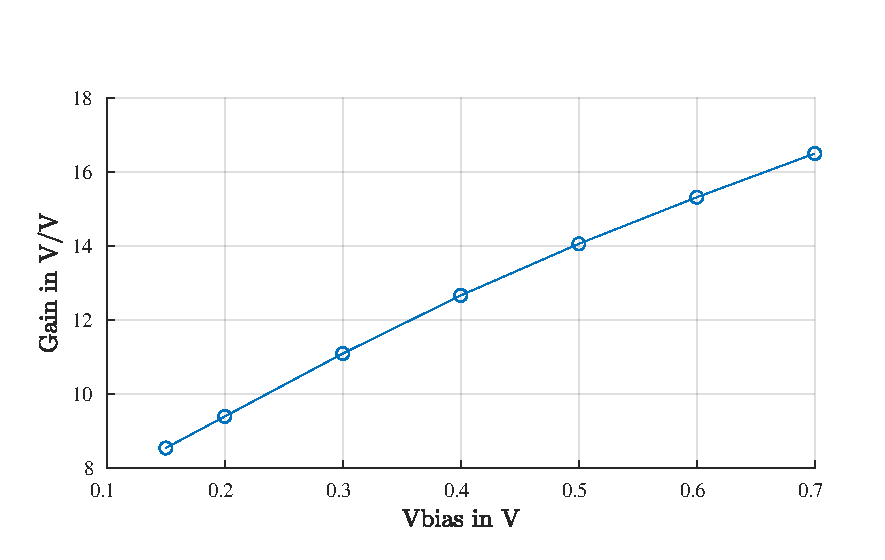
\includegraphics[scale=1]{Figures/Plots/OTA_Gain_Abs.pdf}
\caption{OTA Plot of Gain vs Vbias}
\label{fig:OTA_gain_abs}
\end{figure}

On the same lines, the variation of absolute value of gain with respect to different values of $V_{bias}$ is seen in Figure\ref{fig:OTA_gain_abs} tabulated in Table.\ref{tab:OTA_gain_abs}. The reason to choose the values of $V_{bias}$ are evident from this table and that is because it provides us a gain in the ratio of almost 1:2 for those values of $V_{bias}$. As seen from the table of specifications that we need a transconductance in the ratio of 1:1.8 or something close to that.

\begin{table} [H]
\centering
\begin{tabular}{@{}cccccccc@{}}
\toprule
Vbias (mV)					& 150			& 200			& 300			& 400			& 500			& 600			& 700 \\ \midrule
DC Gain (V/V)			& 8.548		& 9.4		& 11.1		& 12.67		& 14.06		& 15.31		& 16.49 \\
\bottomrule
\end{tabular}
\caption{Absolute values of DC Gain of the OTA}
\label{tab:OTA_gain_abs}
\end{table}

\subsubsection{PSRR}
Figure.\ref{fig:OTA_TB}(c) is the test setup to measure PSRR for a change in $V_{DD}$ and similarly the one in Figure.\ref{fig:OTA_TB}(d) is used to measure PSRR for a change in $V_{SS}$. The circuit conditions are:

$V_{DD}$ = 2.5V; $AC Magnitude$ = 1V; $V_{SS}$ = -2.5V; $V_{cm}$ = 1.95V; $V_{bias}$ = 150mV to 700mV; $C_{L}$ = 50fF.

The variation of PSRR with respect to $V_{bias}$ is tabulated in Table.\ref{tab:OTA_PSRR}. The PSRR is fairly low in the range of nA/V and increases only slightly with increase in $V_{bias}$.

\begin{table} [H]
\centering
\begin{tabular}{@{}cccccccc@{}}
\toprule
Vbias (mV)					& 150			& 200			& 300			& 400			& 500			& 600			& 700 \\ \midrule
PSRR (VDD Supply) (nA/V)			& 234.6		& 236.9		& 241.6		& 246.7 	& 252.2		& 258		& 264.3 \\
PSRR (VSS Supply) (nA/V)			& 254.5		& 256.5		& 260.4		& 264.2		& 267.9		& 271.5		& 274.9 \\
\bottomrule
\end{tabular}
\caption{Power Supply Rejection Ratio of the OTA}
\label{tab:OTA_PSRR}
\end{table}

\subsubsection{Input Impedance}
OTAs generally exhibit a very high input impedance. And to measure this parameter, an AC current source with a magnitude of 1A is connected to the non-inverting terminal of the OTA. And the input impedance is given by the ratio of the AC voltage to the AC current at the input of the OTA. Since the current at the input is 1A, the magnitude of the input voltage will be the value of the input impedance in Ohms at that particular frequency. Since the OTA operation is carried out at 1MHz, the voltage at 1MHz is considered to obtain the value of Input Impedance. Figure.\ref{fig:OTA_TB}(g) shows the test bench to measure the input impedance, with the circuit conditions:

$V_{DD}$ = 2.5V; $V_{SS}$ = -2.5V; $V_{bias}$ = 150mV to 700mV; $C_{L}$ = 50fF; $I_{sin} magnitude$ = 1A. 

The variation of input impedance with respect to $V_{bias}$ is tabulated in Table.\ref{tab:OTA_ZIN}. The variation is quite small and it increases slightly with an increase in bias voltage and is in the order of Mega Ohms.

\begin{table} [H]
\centering
\begin{tabular}{@{}cccccccc@{}}
\toprule
Vbias (mV)					& 150		& 200			& 300			& 400			& 500			& 600			& 700 \\ \midrule
Input Impedance (M$\Omega$)			& 3.38		& 3.388		& 3.403		& 3.419		& 3.434		& 3.45		& 3.467 \\
\bottomrule
\end{tabular}
\caption{Input Impedance of the OTA}
\label{tab:OTA_ZIN}
\end{table}

\subsubsection{Output Impedance}
The output impedance is measured with a help of a current source with unity magnitude at the output instead of a Capacitive load. The differential inputs are connected in a common mode configutation. The test bench to measure the output impedance of the OTA is as shown in Figure.\ref{fig:OTA_TB}(h).

$V_{DD}$ = 2.5V; $V_{SS}$ = -2.5V; $V_{cm}$ = 1.95V $V_{bias}$ = 150mV to 700mV; $I_{sin} magnitude$ = 1A. 
 
As discussed in the theory chapter, OTAs generally have high output impedance. And its variation with respect to $V_{bias}$ is tabulated in the Table.\ref{tab:OTA_ZOUT}
\begin{table} [H]
\centering
\begin{tabular}{@{}cccccccc@{}}
\toprule
Vbias (mV)					& 150		& 200			& 300			& 400			& 500			& 600			& 700 \\ \midrule
Output Impedance (k$\Omega$)			& 1.262		& 1.3		& 1.382		& 1.473		& 1.577		& 1.697		& 1.837 \\
\bottomrule
\end{tabular}
\caption{Output Impedance of the OTA}
\label{tab:OTA_ZOUT}
\end{table}

\subsection{Noise Analysis}

Once again, we use the same test bench as shown in Figure.\ref{fig:OTA_TB}(a) to perform the noise analysis. As mentioned in the previous sections of this chapter, the NMOS differential pair exhibits high flicker noise, also known as 1/f noise. This noise is significant at low frequencies. At moderate and high frequencies, the effect of thermal or white noise is much more dominant and hence flicker noise becomes less significant at those frequencies.

The variation of the input referred noise with respect to $V_{bias}$ is tabulated in Table.\ref{tab:OTA_Noise}. With increase in $V_{bias}$, the input referred noise decreases. This is because the gain increases with increase in $V_{bias}$ and consequently input referred noise decreases. This also converges to the fact that the input referred noise decreases with bigger dimensions of the differential pair, and thereby contributing to a higher gain.

\begin{table} [H]
\centering
\begin{tabular}{@{}cccccccc@{}}
\toprule
Vbias (mV)					& 150			& 200			& 300			& 400			& 500			& 600			& 700 \\ \midrule
Input Referred Noise (nV/$\sqrt{Hz}$)			& 46.36		& 43.73		& 39.83		& 37.29		& 35.57		& 34.31		& 33.28 \\
\bottomrule
\end{tabular}
\caption{Input Referred Noise of the OTA}
\label{tab:OTA_Noise}
\end{table}

\subsection{Transient Analysis}
For the OTA designed, the transient analysis is performed for sine wave input and square wave input. The test bench in Figure.\ref{fig:OTA_TB}(e) and (f) is used to perform the transient analysis of the designed OTA.

\subsubsection{Sine Input}
The test bench in Figure.\ref{fig:OTA_TB}(e) is used to measure the transient parameters for a sine wave input with the circuit conditions as shown below. An ideal balun is used at the input to provide a differential voltage to the terminals. The voltages are 180$^0$ out of phase with each other. 

$V_{DD}$ = 2.5V; $V_{SS}$ = -2.5V; $V_{cm}$ = 1.95V; $V_{bias}$ = 150mV to 700mV;  $V_{sin} amplitude$ = 100mV; $frequency = 1MHz$ $C_{L}$ = 50fF.

The transient simulation is carried out for 3$\mu $s. The sinusoidal output with respect to time is shown in Figure.\ref{fig:OTA_Sine} for different values of $V_{bias}$. As we know from the AC analysis, the gain varies in the ratio of 1:2 and thereby, here we have the peak-to-peak voltages varying in the same ratio. And as discussed in the DC Analysis, the DC bias points at the output are close to zero but not exactly at 0 for all the $V_{bias}$ values.

\begin{figure} [H]
\centering
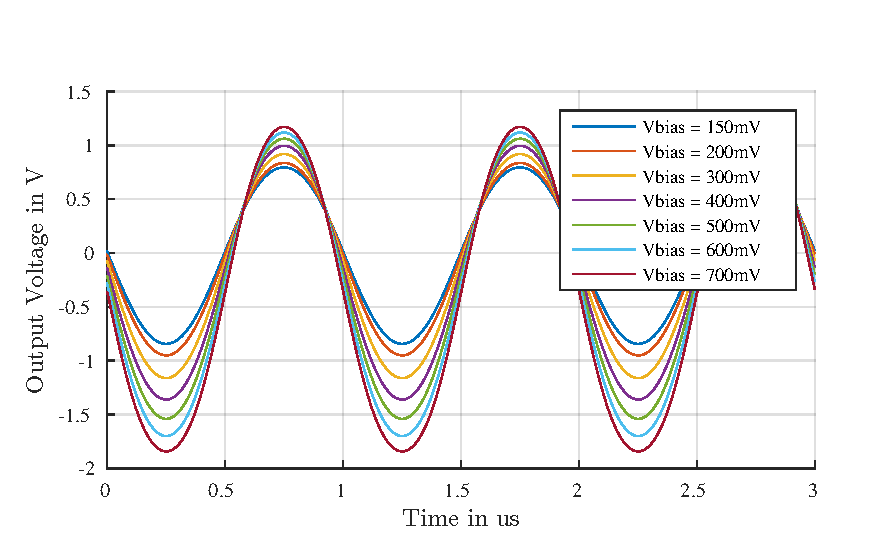
\includegraphics[scale=1]{Figures/Plots/OTA_Sine.pdf}
\caption{OTA Output Voltage for vs time for different Vbias}
\label{fig:OTA_Sine}
\end{figure}

Table\ref{tab:OTA_Sine_Params} shows the variation of different transient parameters with respect to $V_{bias}$. The voltage swing varies from 1.639 to 3.014 which is almost in the ratio of 1:2. HD3 worsens with increase in $V_{bias}$ and on the contrart, improves. Although, it is seen that the HD2 again starts to worsen beyond 600mV of $V_{bias}$.

\begin{table} [H]
\centering
\begin{tabular}{@{}cccccccc@{}}
\toprule
Vbias (mV)					& 150			& 200			& 300			& 400			& 500			& 600			& 700 \\ \midrule
Vout Max (V)			& 0.7949		& 0.8362		& 0.9188		& 0.995		& 1.061		& 1.119		& 1.172 \\
Vout Min (V)			& -0.844		& -0.9505		& -1.162		& -1.361		& -1.54		& -1.7		& -1.842 \\
Vout Swing (V)				& 1.639		& 1.787		& 2.081		& 2.356		& 2.601		& 2.818		& 3.014 \\
HD2 (dBc) 				& -44.83		& -44.28		& -43.86		& -44.74		& -47.97		& -60.86		& -48.75 \\
HD3 (dBc) 				& -52.15		& -49.69		& -46.13		& -43.87		& -42.24		& -40.78		& -39.32 \\
\bottomrule
\end{tabular}
\caption{Transient Parameters of the OTA}
\label{tab:OTA_Sine_Params}
\end{table}

\subsubsection{Square Input}
The test bench in Figure.(f) is used to measure the transient parameters for a square wave input. Slew rate is the rate of change of output voltage. It is also defined as the ratio of bias current to load capacitance.

$V_{DD}$ = 2.5V; $V_{SS}$ = -2.5V; $V_{cm}$ = 1.95V; $V_{bias}$ = 150mV to 700mV;  $V_{pulse} V_1$ = 100mV; $V_2$ = -100mV; $Pulse Width$ = 49.7ns; $Period$ = 100ns; $Rise Time$ = 300ps; $Fall time$ = 300ps; $C_{L}$ = 50fF.

The slew rate, both for the rising edge and the falling edge is tabulated in the Table.\ref{tab:OTA_Slew}. The OTA is reasonably fast enough high $V_{bias}$ voltages.

\begin{table} [H]
\centering
\begin{tabular}{@{}cccccccc@{}}
\toprule
Vbias (mV)					& 150			& 200			& 300			& 400			& 500			& 600			& 700 \\ \midrule
Slew Rate Rising Edge (V/us)			& 386.9		& 407.8		& 452.9		& 501.9 	& 547.6		& 585.4		& 609.3 \\
Slew Rate Falling Edge (V/us)			& -389		& -413.8		& -469.4		& -523.5		& -570.5		& -605.7		& -626.4 \\
\bottomrule
\end{tabular}
\caption{Slew Rate of the OTA}
\label{tab:OTA_Slew}
\end{table}

\section{Summary}
\begin{table} [H]
\centering
\begin{tabular}{@{}ccc@{}}
\toprule
Parameter						& Programmable Voltage	\\ \midrule
Linear Input Voltage Range		& $\pm$100 mV			\\
Bandwidth						& 89.19 .. 135 MHz				\\
Slew Rate						& $\pm$386.6 .. 609.3 V/$\mu$s	\\
Input Referred Noise			& 33.28 .. 46.64 nV/$\sqrt{Hz}$ @1MHz \\
Input Impedance					& 3.38 .. 3.467 M$\Omega$		\\
Output Impedance				& 1.262 .. 1.837 K$\Omega$		\\
Output Voltage Swing			& 1.6389 .. 3.014 V				\\
HD2								& -43.86 .. -60.86 dBc			\\
HD3								& -39.32 .. -52.15 dBc			\\
Open Loop Voltage Gain			& 8.548 .. 16.49 V/V			\\
PSRR							& 234.6 .. 274.9 nA/V			\\
\bottomrule
\end{tabular}
\caption{Simulation Results of the OTA}
\label{tab:Results}
\end{table}

\subsubsection{Conclusion}
The obejective of the first stage of the system was to design a programmable operational transconductance amplifier. The OTA was used in voltage mode. Different topologies were considered and the best fit according to the requirements and the complexity was chosen - the conventional current mirror based OTA. The intial design challenge was choosing the topology of the overall system - whether a single stage would be sufficient or a two stage is necessary. With a single stage, the OTA can only drive capacitive loads and for high currents, a large value of load capacitance is necessary and thus reducing the overall bandwidth for the ouput current. Using the OTA in voltage meant that the output voltage swing variation should be in the ratio of 1:1.8 (Transconductance specification). To achieve this ratio, the range of bias current chosen came down to the effects of DC bias voltage at the output and also the gain of the OTA. Having done all these, the output voltage swing requirement from the first stage was achieved but with a $\pm$100mV linear input voltage range. The operating bandwidth of the system was higher than the required specification so that it makes up for the dominant pole of the second stage.

\chapter{Operational Amplifier}

\section{Design and Implementation}
With the gain of the first stage suffieciently high enough, the second stage is used just as a buffer. The high impedance output of the operational transconductance amplifier has to be converted to a low impedance output in order to drive a resistive load instead of a pure capacitive load. The first thing to ponder upon is the specifications to design the op amp. And then from the specifications, we can decide on a possible topology for the op amp. So how to arrive at the specifications is the question. We have the results from the first stage OTA and since the output of the OTA is directly provided to the input of the op amp, we can use the OTA to generate the specifications of the op amp. Some of the trivial things like the input common mode range and the output voltage swing can be directly obtained by looking at the output of the OTA. But some of the key parameters like the open loop gain, gain bandwidth prodcut, slew rate, etc., need simulations to reach our requirement. The output impedance, the output current range specifications can be directly taken from the system specifications tabulated in Chapter 1.

\begin{figure} [H]
\centering
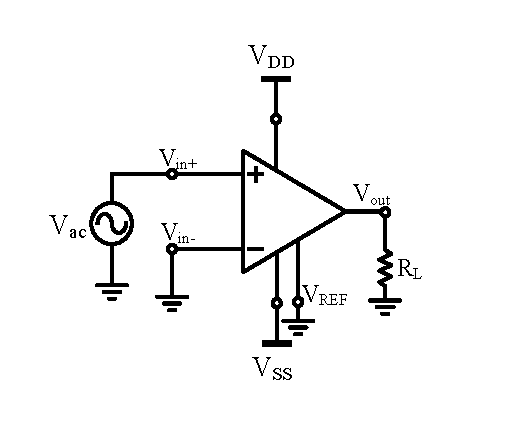
\includegraphics[scale=1]{Figures/System_Level/ahdl_OPAMP.pdf}
\caption{Behavior Modelling of Ideal OP AMP}
\label{fig:ahdlopamp}
\end{figure}

Cadence Virtuoso offers a few basic libraries and ahdllib (analog hdl library) is one of them. The ahdllib offers an ideal op amp which can used for behavior modelling to sweep gain, unity bandwidth, input impedance, and slew rate. The test setup for this modelling is as shown in Figure.\ref{fig:ahdlopamp}. The $V_{REF}$ reference voltage is typically used to set the DC level of the OP AMP. Generally, the middle voltage between $V_{DD}$ and $V_{SS}$ is the value set for $V_{REF}$. And in this case, as we have a dual bipolar supply, the $V_{REF}$ is grounded. The other behavioral inputs to these are the open loop gain, unity gain bandwidth, input impedance, output impedance, bias current, slew rate, maximum output current. The open loop gain, unity gain bandwidth, slew rate are swept over a wide range of values with input impedance a value much higher than the output impedance of the OTA. The bias current is set to zero and the maximum output current is left unset. The OTA designed is cascaded with the ideal OP AMP by connecting the output pin of the OTA to the non-inverting terminal of the ideal OP AMP. The unity gain bandwidth of the OP AMP that provides the overall system bandwidth that matches the specification is is the unity bandwidth with which the OP AMP has to be designed. And likewise, the value of gain that stabilizes the overall system is the open loop gain of the op amp to be designed. Following the steps above, the specifications of the OP AMP to be designed are tabulated  below.

\begin{table} [H]
\centering
\begin{tabular}{@{}cc@{}}
\toprule
Parameter					& Value				\\ \midrule
Open Loop Gain				& 30 dB				\\
Gain Bandwidth Product		& 6 MHz				\\
ICMR (min)					& -1.85 V			\\
ICMR (max)					& 1.2 V				\\
Output Voltage Swing		& -2 .. 2 			\\
Slew Rate					& 900 V/us			\\
Input Impedance				& 10 M$\Omega$		\\
Output Impedance			& 55 K$\Omega$		\\
\bottomrule
\end{tabular}
\caption{Specifications of the OPAMP to be designed}
\label{tab:OPAMP_Specs}
\end{table}

The two-stage circuit architecture has historically been the most popular approach to op amp design. The main reason for that being it can provides a very high gain and a high output swing. The two stages refer to the number of gain stages in the op amp. An optional output buffer to the op amp can be used as a third stage. 

Optimal compensation of op amps are arguably one of the most difficult parts of a design. Two most popular approaches are dominant pole compensation and lead compensation. Compensation capacitor between the output of the gain stages causes pole-splitting and achieves dominant pole compensation. This capacitor is known as Miller capacitor and the op amp is called as a two stage Miller compensation op amp. With the use of this compensation capacitor, the location of the poles can be chosen and thereby the bandwidth of the op amp can be set according to our requirements. This is important because the we need a 6MHz unity gain bandwidth from the OP AMP to meet our requirements and to get a stable enough system.

\subsection{Schematic}
The schematic of the Miller compensation op amp is as shown in the Figure.\ref{fig:OPAMP_Schematic}. The bias current to the differential pair is provided through the current mirror pair of $M_5$ and $M_8$. The bias current is controlled through the transistor $M_9$ whose gate voltage is provided by the voltage divider formed by the resistors $R_{b1}$ and $R_{b2}$. The adaptive load for the differential stage is formed by the current mirror pair $M_3$ and $M_4$. The second stage is the common source amplifier formed by the transistors $M_6$ and $M_7$. $C_C$ is the compensation capacitor connected between the output of the two stages of the amplifier. The phase margin can be set by adjusting the value of this capacitor.  Smaller the capacitor, higher the phase margin of the op amp. The dimensions of the differential pair are chosen with the help of the graphs generated using the $G_m/I_D$ methodology to obtain the a moderate gain and required unity gain bandwidth. The adaptive load sets the maximum input common mode voltage and $M_5$ sets the minimum input common mode voltage. The output voltage range is set by the common source amplifier and therefore the open loop gain. $M_6$ is tweaked to alter the gain of the op amp. Alternatively the gain is also increased by decreasing the bias current. And then in order to maintain the voltage swing, the W/L ratios of some transistors need tuning as well.

\begin{figure} [H]
\centering
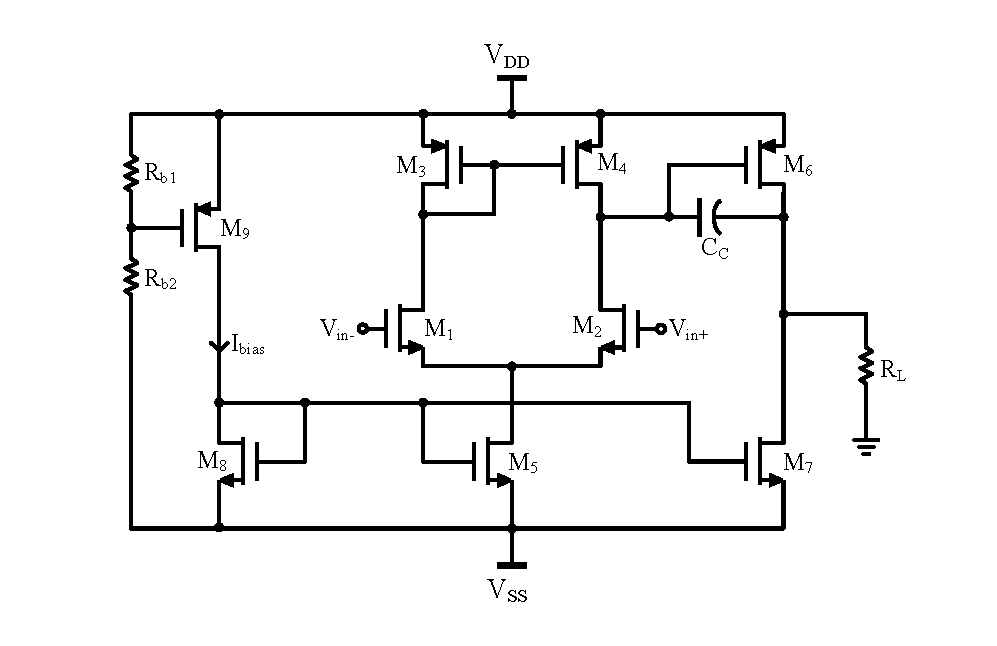
\includegraphics[scale=1]{Figures/Schematics/OPAMP_Vbias.pdf}
\caption{Schematic of the OPAMP Designed}
\label{fig:OPAMP_Schematic}
\end{figure}

The dimensions of the transistors are tabulated in Table.\ref{tab:OPAMP_dimensions}. One can easily recognize that the transistors at the output are significantly large. This is designed so to make sure the op amp provides a very high current and thereby avoiding a common collector amplifier at the output of the op amp to amplify the output current. The compensation capacitance value is 50fF.

\begin{table} [H]
\centering
\begin{tabular}{@{}cccc@{}}
\toprule
Transistor			& Width($\mu$m)		& Length(nm)		& Multiplier \\ \midrule
M1					& 5					& 500				& 2			\\
M2					& 5					& 500				& 2			\\ 
M3					& 30 				& 500				& 1			\\
M4					& 30 				& 500				& 1			\\ 
M5					& 2 				& 500				& 1			\\
M6					& 85 				& 500				& 55		\\ 
M7					& 50 				& 500				& 48		\\
M8					& 2 				& 500				& 1			\\ 
M9					& 0.7				& 500				& 1			\\
\bottomrule
\end{tabular}
\caption{Dimensions of the Transistors of the designed OPAMP}
\label{tab:OPAMP_dimensions}
\end{table}

\section{Test Setup}
\begin{figure} [H]
\centering
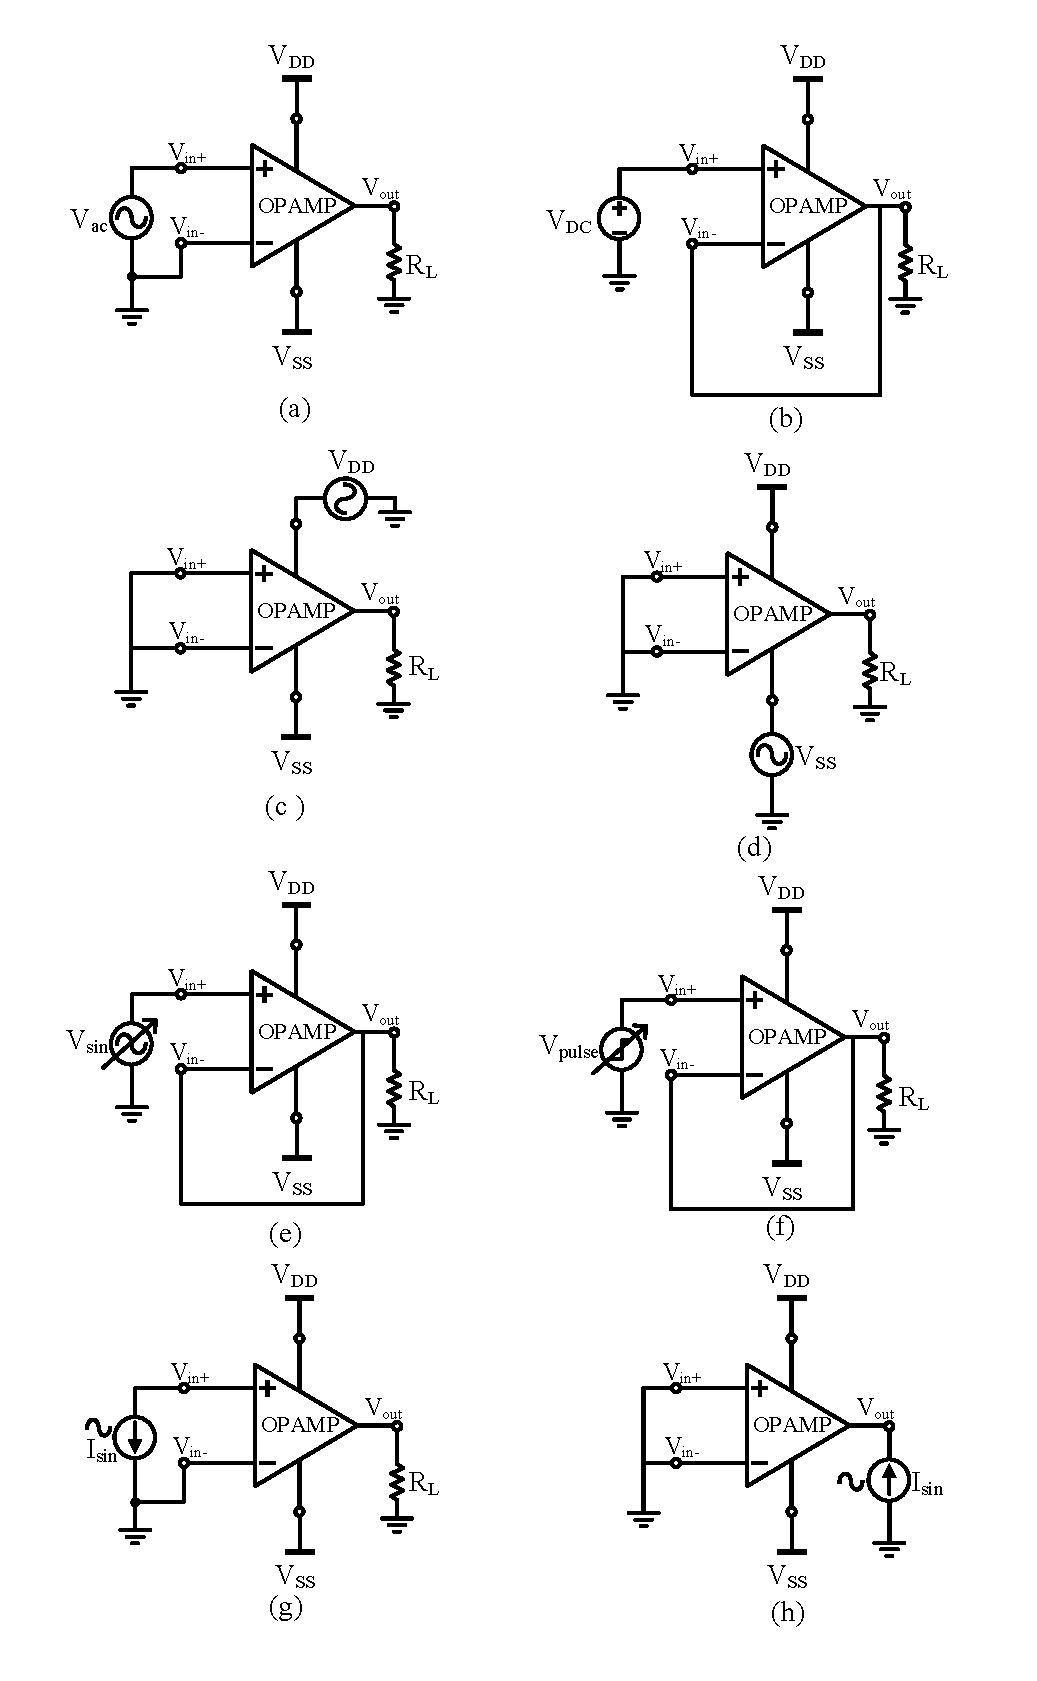
\includegraphics[scale=0.8]{Figures/Test_Benches/OPAMP_TB.pdf}
\caption{Test bench setup for OP AMP}
\label{fig:OPAMP_TB}
\end{figure}

The test bench setup for the operation transconductance amplifier is as shown in Figure.\ref{fig:OPAMP_TB}. All the analyses are carried out under a standard temperature of $27_0C$, typical mean conditions for the NMOS transistors, PMOS transistors, capacitors and resistors unless explicitly mentioned otherwise. The $ocean$ script containing all the expressions to measure the various parameters of the OP AMP are attached in the Appendix. In the following subsections, the results of these parameters are discussed using DC Analysis, AC Analysis, Transient Analysis and Noise Analysis separately.

\subsection{DC Analysis}
The OP AMP is not separately biased. The DC level at the output of the OTA cannot be filtered out using a coupling capacitor as the OTA is already driving a capacitive load. Therefore the common mode voltage of the OP AMP will be the DC output bias of the OTA. Considering that the OP AMP is connected in a buffer configuration, the output of the OP AMP will have the same DC level as the output of the OTA. As part of the DC analysis, the input common mode range and the output voltage swing is calculated. In the test circuit in Figure.\ref{fig:OPAMP_TB}(b), the input DC voltage is varied from $V_{SS}$ to $V_{DD}$ and the voltage range in the linear range varies from -2.19V to 2.089V. Similarly the output voltage swing is calculated without the negative feedback and is found to be -2.19V and 2.323V.

$V_{DD}$ = 2.5V; $V_{SS}$ = -2.5V; $V_{DC}$ = -2.5V to 2.5V; $R_L$ = 50$\Omega$.
\begin{table} [H]
\centering
\begin{tabular}{@{}cc@{}}
\toprule
Parameter					& Value				\\ \midrule
ICMR (min)					& -2.19 V			\\
ICMR (max)					& 2.089 V			\\
Output Voltage Swing		& -2.19 .. 2.323V	\\
\bottomrule
\end{tabular}
\caption{DC Analysis}
\label{tab:OPAMP_DC}
\end{table}

\subsection{AC Analysis}
\subsubsection{Gain and Unity Bandwidth}
The open loop gain and the gain bandwidth product are inarguably the most important parameters of an operational amplifier. The test bench used to measure these parameters is as shown in Figure.\ref{fig:OPAMP_TB}(a). The op amp is configured in an open loop. The DC biasing to the differential transistor pair is provided by the output of the OTA, which is centred around 0V. 

The plot of the open loop gain and the phase of the op amp is as shown in the Figure.\ref{fig:OPAMP_gain_pm_gbw}. The open loop gain of the op amp is 30.8dB. The gain bandwidth product is 6.2MHz and correspondingly the phase margin is $76.79^0$.

$V_{DD}$ = 2.5V; $V_{SS}$ = -2.5V; $V_{ac} magnitude $ = 1 V; $R_L$ = 50$\Omega$.
\begin{figure} [H]
\centering
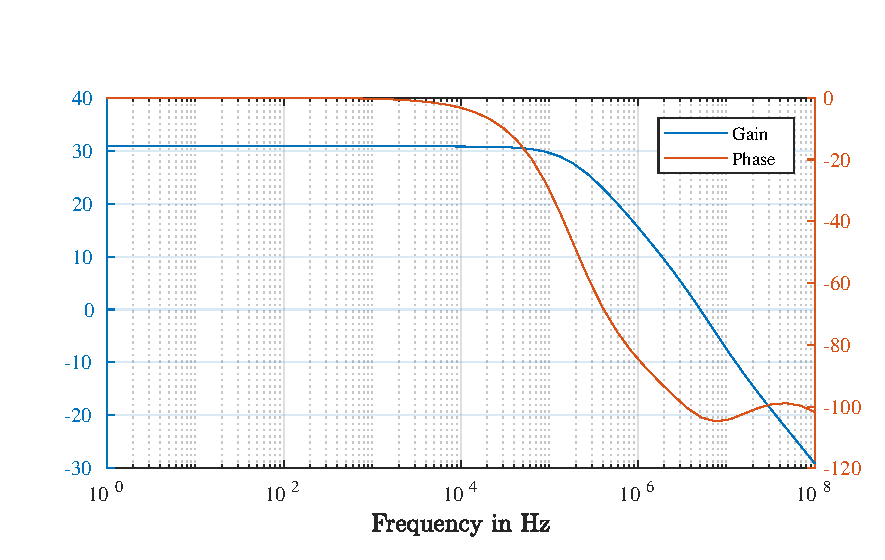
\includegraphics[scale=1]{Figures/Plots/OPAMP_Gain_PM.pdf}
\caption{OPAMP Plot of Gain and Phase vs Frequency}
\label{fig:OPAMP_gain_pm_gbw}
\end{figure}

\begin{table} [H]
\centering
\begin{tabular}{@{}cc@{}}
\toprule
Parameter					& Value				\\ \midrule
Open Loop Gain				& 30.8 dB			\\
Phase Margin				& 76.79 degrees		\\
Unity Gain Bandwidth		& 6.2 MHz			\\
\bottomrule
\end{tabular}
\caption{Gain and Unity Bandwidth of the OP AMP}
\label{tab:OPAMP_Gain_UBW}
\end{table}

\subsubsection{PSRR}
The PSRR of the OTA in the first stage was in the range of $nA/V$ and hence neglibigle. However, the op amp designed exhibits a relatively high value of PSRR. This is due to the bulky transistors at the output stage. The test bench to measure the PSRR of the op amp is as shown in the Figure.\ref{fig:OPAMP_TB}(c) and (d); (c) is used to measure PSRR for a change in $V_{DD}$ and similarly, (d) is used to measure PSRR for a change in $V_{SS}$.

$V_{DD}$ = 2.5V; $V_{SS}$ = -2.5V; $V_{ac} magnitude $ = 1 V; $R_L$ = 50$\Omega$.

\begin{table} [H]
\centering
\begin{tabular}{@{}cc@{}}
\toprule
Parameter					& Value				\\ \midrule
PSRR($V_{DD}$)				& 30.96 $\mu$A/V		\\
PSRR($V_{SS}$)				& 138.8 $\mu$A/V		\\
\bottomrule
\end{tabular}
\caption{PSRR of the OP AMP}
\label{tab:OPAMP_PSRR}
\end{table}

\subsubsection{Input and Output Impedance}
The test bench to calculate the input impedance follows a similar concept to that of the OTA. i.e., a unity current source is connected to the non-inverting terminal of the op amp and the voltage at that terminal is measured which in turn is the magnitude of the input impedance of the op amp.

To have a stable system, it is important that input impedance of the second stage is higher than the output impedance of the first stage. Given that the output impedance of the OTA is generally high, the input impedance of the op amp becomes a very important parameter. And the input impedance is found to be 9.04M$\Omega$.

$V_{DD}$ = 2.5V; $V_{SS}$ = -2.5V; $I_{sin} magnitude $ = 1A.

Op amps are known to have zero or very low output impedance. Along with this theoretical fact, the op amp in this work is designed to have very high output currents, so it is expected to have a very low output impedance. The value of the output impedance is observed to be 4.167$\Omega$.

\subsection{Transient Analysis}
The test bench to perform the transient analysis is as shown in the Figure.\ref{fig:OPAMP_TB}(e). The op amp is connected in a negative feedback configuration so as to analyse its behavior as a voltage buffer.

$V_{DD}$ = 2.5V; $V_{SS}$ = -2.5V; $V_{sin} amplitude $ = 1.5V; $frequency$ = 1MHz; $R_L$ = 50$\Omega$.

The output current of the op amp is effectively the current flowing through the load resistor $R_L$. The plot of current versus time is as shown in the Figure.\ref{fig:OPAMP_Iout}. The current is $180^0$ out of phase with the voltage and it ranges from -30mA to 30mA for a 50$\Omega$ load and 3V peak to peak input voltage. 

\begin{figure} [H]
\centering
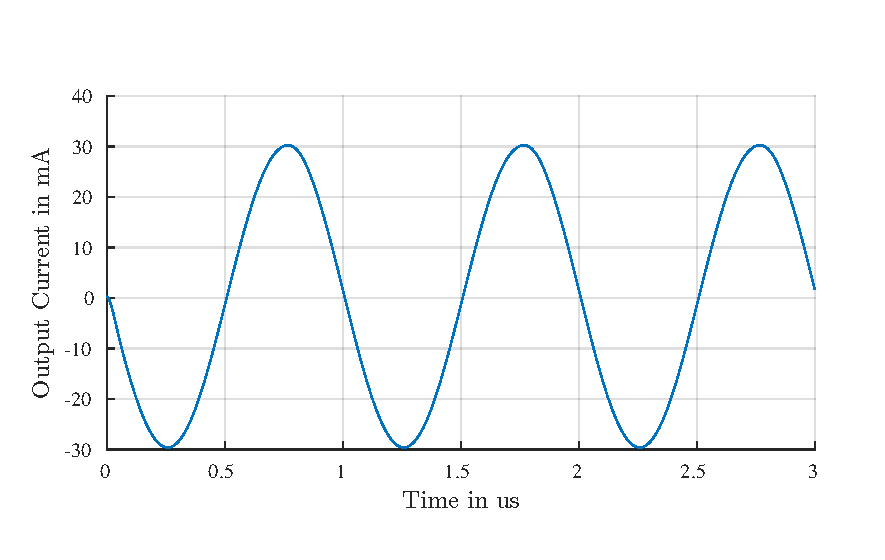
\includegraphics[scale=1]{Figures/Plots/OPAMP_Iout.pdf}
\caption{OPAMP Plot of Ourput Current vs time}
\label{fig:OPAMP_Iout}
\end{figure}

\section{Summary}

The values of all the parameters of the op amp discussed so far have been tabulated in Table.\ref{tab:OPAMP_Results}
\begin{table} [H]
\centering
\begin{tabular}{@{}cc@{}}
\toprule
Parameter					& Value				\\ \midrule
Open Loop Gain				& 30.8 dB			\\
Gain Bandwidth Product		& 6.2 MHz			\\
Phase Margin				& 76.79				\\
ICMR (min)					& -2.19 V			\\
ICMR (max)					& 2.089 V			\\
Output Current (max)		& -29.6 mA			\\
Output Current (min)		& 30.28 mA			\\
Output Voltage Swing		& -2.19 .. 2.323 	\\
Slew Rate					& 10 V/us			\\
PSRR (VDD)					& 30.96 uA/V		\\
PSRR (VSS)					& 138.8 uA/V		\\
Input Impedance				& 9.04 MOhms		\\
Output Impedance			& 4.167 Ohms		\\
\bottomrule
\end{tabular}
\caption{Simlation Results of the OPAMP}
\label{tab:OPAMP_Results}
\end{table}

\chapter{Overall System}

The block diagram of the two stage design with an OTA and an OP AMP is as shown in Figure.\ref{fig:System_Block_Diagram}. The other end of the capacitor of the first stage is connected to the negative power supply instead of ground since we have only two levels in the IC (-2.5V and 2.5V). Both the stages use the same power supply. The output of the OTA is directly connected to the non-inverting terminal of the OP AMP without any DC isolation via a coupling capacitor.

\begin{figure} [H]
\centering
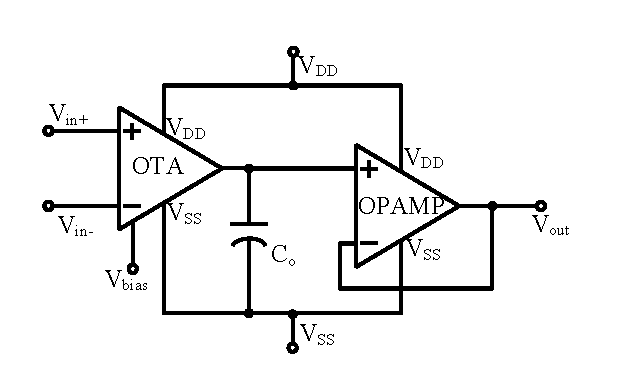
\includegraphics[scale=1]{Figures/System_Level/System_Overview.pdf}
\caption{Block Diagram of the Overall System}
\label{fig:System_Block_Diagram}
\end{figure}

The schematic symbol for the overall system is as indicated in Figure.\ref{fig:System_Symbol}. The block diagram of the system is drawn inside to get an understanding of the configuration.

\begin{figure} [H]
\centering
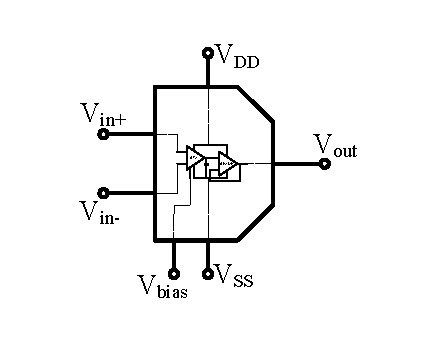
\includegraphics[scale=1]{Figures/System_Level/System_Symbol.pdf}
\caption{Schematic Symbol for the Overall System}
\label{fig:System_Symbol}
\end{figure}

\section{Schematic}
The transistor level schematic of the overall system is as shown in the Figure.\ref{fig:System_Schematic}. The upper portion of the schematic is the OTA and the bottom portion is the OP AMP. Note the feedback connection of the OP AMP and the connection between the OTA and the OP AMP. To summarize the physical aspects of the system, there are 3 input terminals, 2 power supply levels and 1 ouput pin.
 
\begin{figure} [H]
\centering
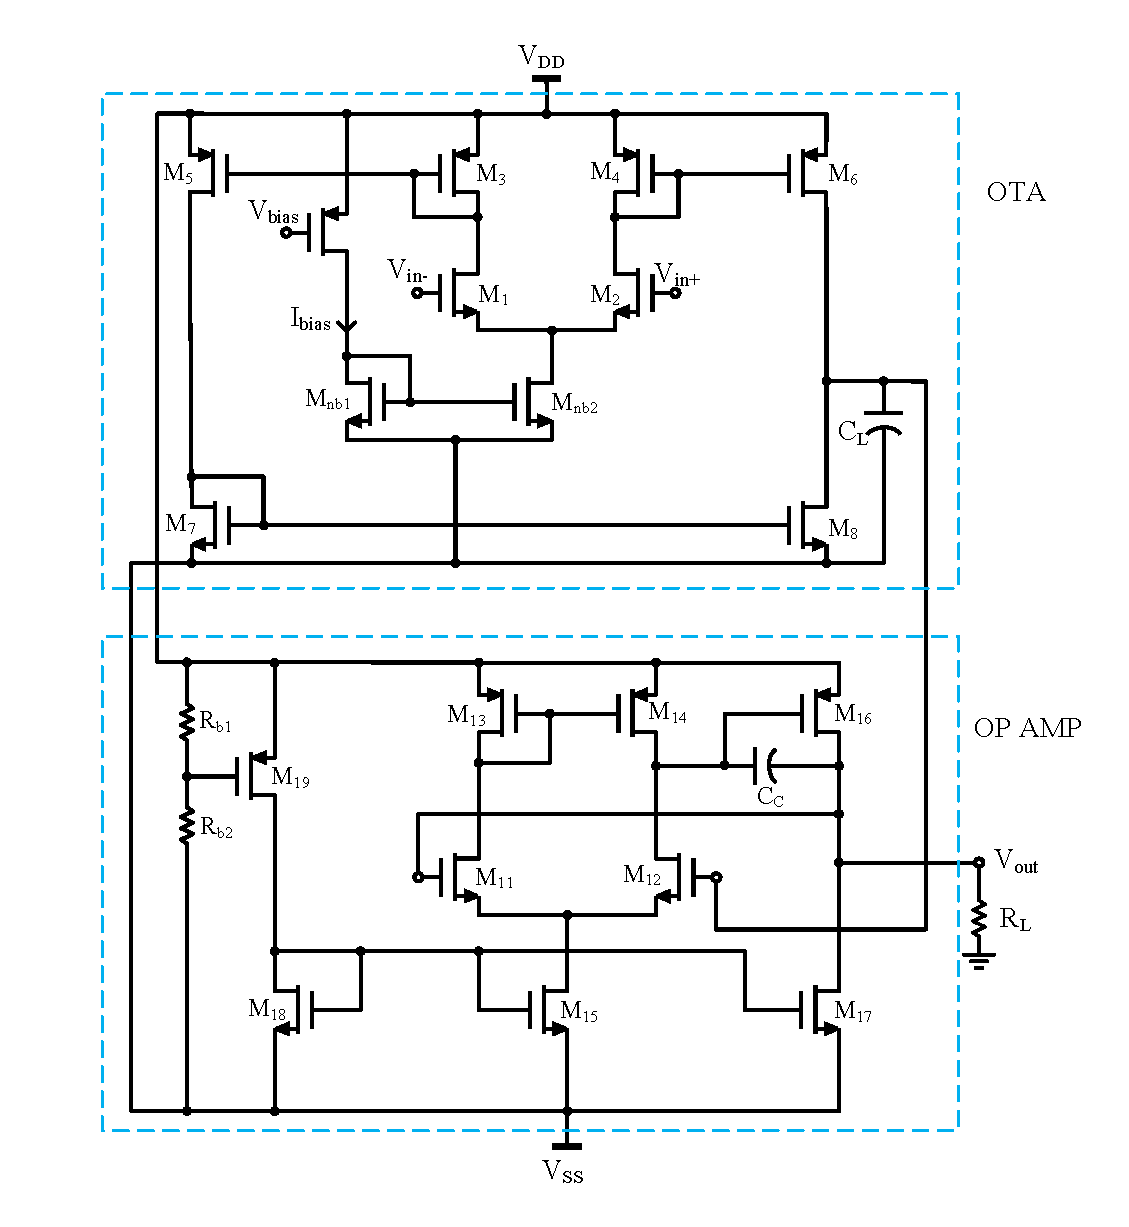
\includegraphics[scale=1]{Figures/Schematics/OTA_OPAMP_Schematic_RL.pdf}
\caption{Schematic Diagram for the Overall System}
\label{fig:System_Schematic}
\end{figure}

\section{Test Setup}

\begin{figure} [H]
\centering
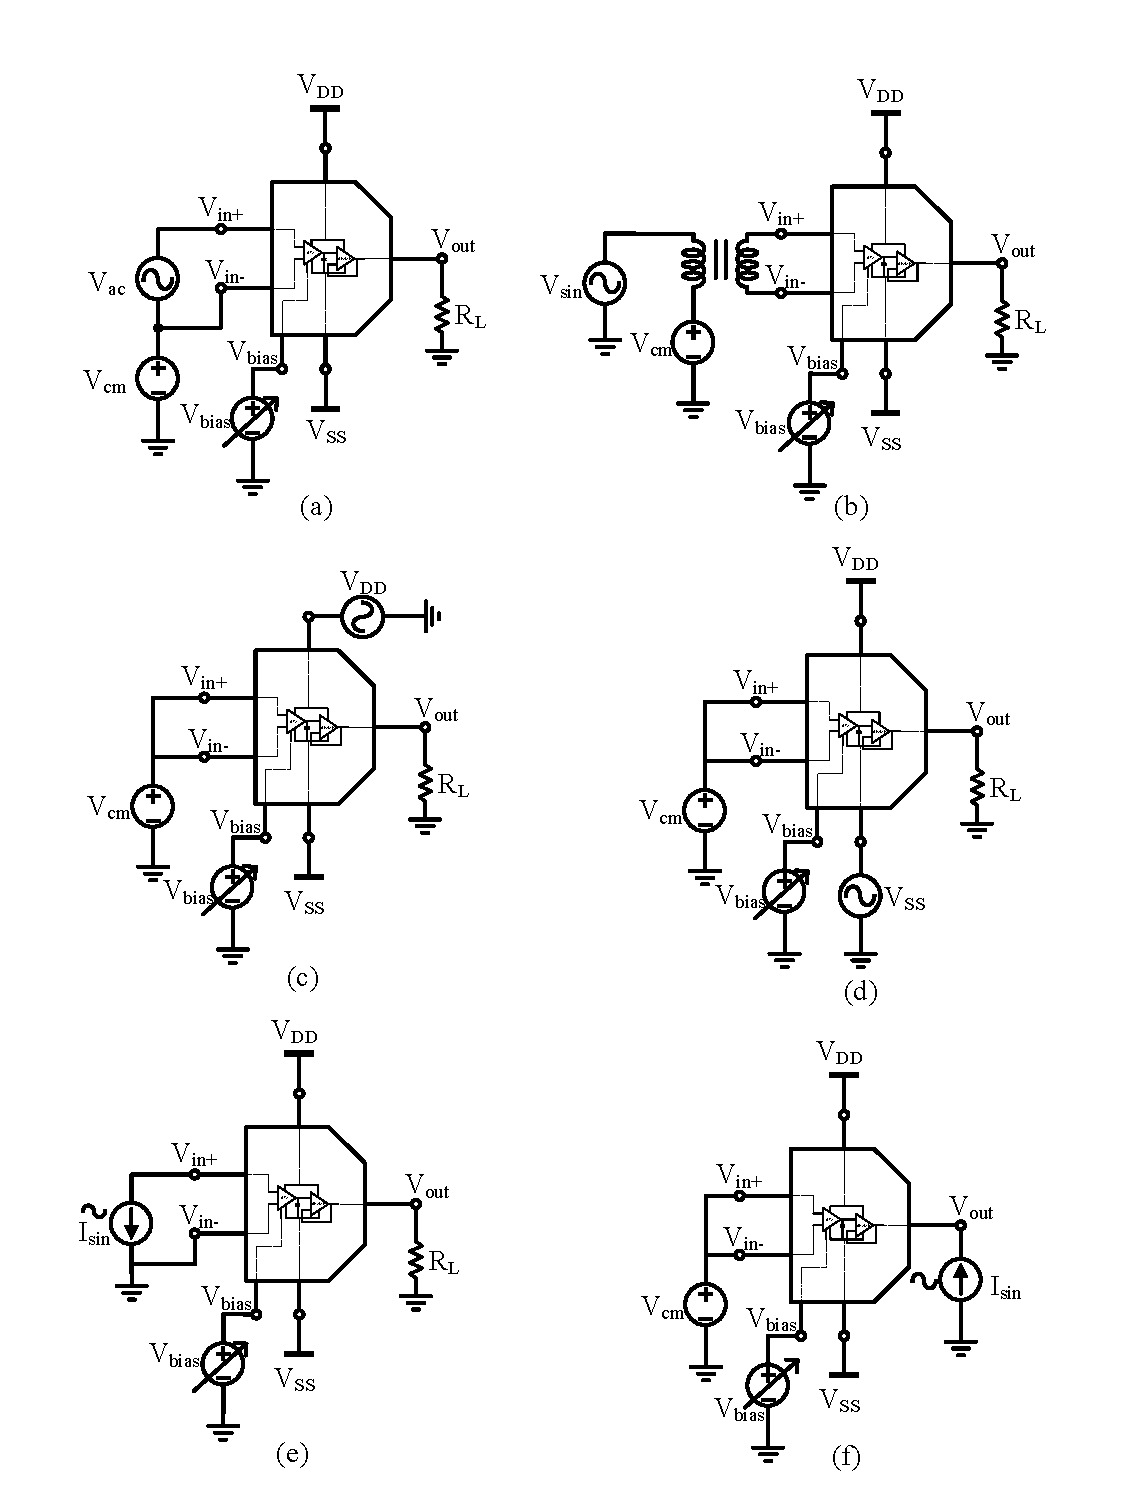
\includegraphics[scale=0.9]{Figures/Test_Benches/Overall_TB.pdf}
\caption{Test setup for DC Analysis}
\label{fig:TB}
\end{figure}

\subsection{DC Analysis}
The test bench to perform the DC analysis is as shown in the Figure.(a). 

$V_{DD}$ = 2.5V; $V_{SS}$ = -2.5V; $V_{cm}$ = 1.95V; $V_{bias}$ = 150mV to 700mV;  $V_{ac}$ = 1V; $R_{L}$ = 50$\Omega$.

The DC Bias point at the output of the system is tabulated in the Table.\ref{tab:DC}. Output DC bias points are almost symmetric around 0V and vary from 180.1mV to -219.3mV.
\begin{table} [H]
\centering
\begin{tabular}{@{}cc@{}}
\toprule
Vbias (mV)			& Output DC Bias (mV)	\\ \midrule
150					& 180.1  \\
200					& 148.4  \\
250					& 115.8  \\
300					& 82.28	 \\
350					& 47.83	 \\
400					& 12.45	 \\
450					& -23.86 \\
500					& -61.08 \\
550					& -99.24 \\
600					& -138.3 \\
650					& -178.4 \\
700 				& -219.3 \\
\bottomrule
\end{tabular}
\caption{DC Bias Point at the output of the circuit}
\label{tab:DC}
\end{table}

\subsection{AC Analysis}

The test bench in Figure.(a) is used for the AC analysis too. The magnitude of the AC source is set to 1V and as mentioned in the previous chapter, the voltage at the output will be the gain of the overall system.

The plot of gain for different values of $V_{bias}$ is as shown in the Figure.\ref{fig:Gain}. The value of the open loop gain is between 18dB and 25dB.

\begin{figure} [H]
\centering
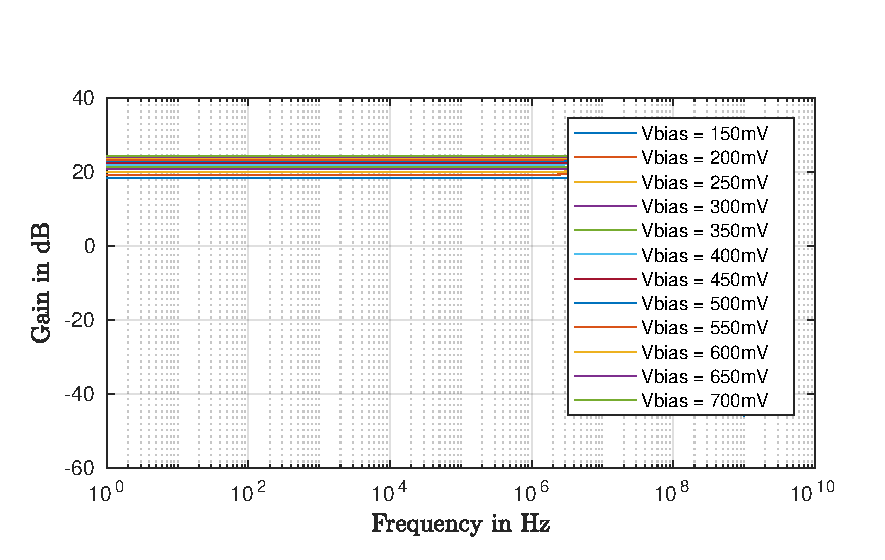
\includegraphics[scale=1]{Figures/Plots/Ov_Gain.pdf}
\caption{Plot of Gain vs Frequency for different Vbias}
\label{fig:Gain}
\end{figure}
The results of the AC analysis are tabulated below in Table.\ref{tab:GAIN_GBW_PM}. The bandwidth is fairly constant at around 14MHz. But the phase margin starting to drop just a tad below 30 with a $V_{bias}$ of 700mV and beyond. 
\begin{table} [H]
\centering
\begin{tabular}{@{}cccc@{}}
\toprule
Vbias (mV)			& DC Gain (dB) 	& Bandwidth (MHz) 	& Phase Margin \\ \midrule
150					& 18.5  		& 14.43 			& 55.49 \\
200					& 19.34			& 14.38 			& 51.37 \\
250					& 20.13  		& 14.34 			& 47.76 \\
300					& 20.83	 		& 14.29 			& 45.08 \\
350					& 21.46			& 14.24 			& 42.55 \\
400					& 22.02	 		& 14.19 			& 40.19 \\
450					& 22.52 		& 14.14 			& 38	\\
500					& 22.97 		& 14.08 			& 35.97	\\
550					& 23.38 		& 14.01 			& 34.08 \\
600					& 23.75 		& 13.95 			& 32.31 \\
650					& 24.1 			& 13.88 			& 30.63 \\
700 				& 24.43 		& 13.8  			& 29.02 \\
\bottomrule
\end{tabular}
\caption{DC Gain, Bandwidth and Phase Margin of the Overall System}
\label{tab:GAIN_GBW_PM}
\end{table}

The test bench in Figure.(e) is used to measure the input impedance of the system. The concept for measurement is same as in the case of the OTA. The voltage at the non-inverting terminal will be the magnitude of the input impedance of the overall system because the magnitude of the current from the AC source is 1A.

$V_{DD}$ = 2.5V; $V_{SS}$ = -2.5V; $V_{bias}$ = 150mV to 700mV;  $I_{sin} magnitude$ = 1A; $R_{L}$ = 50$\Omega$.


The value of input impedance with respect to Vbias is tabulated in Table.\ref{tab:ZIN}. It is clear that the input impedance of the overall system is same as the input impedance of the OTA in the first stage.

\begin{table} [H]
\centering
\begin{tabular}{@{}cc@{}}
\toprule
Vbias (mV)			& Input Impedance (M$\Omega$)	\\ \midrule
150					& 3.394  \\
200					& 3.402  \\
250					& 3.41   \\
300					& 3.418	 \\
350					& 3.425	 \\
400					& 3.433	 \\
450					& 3.44  \\
500					& 3.448 \\
550					& 3.456 \\
600					& 3.464 \\
650					& 3.473 \\
700 				& 3.482 \\
\bottomrule
\end{tabular}
\caption{Input Impedance of the Overall System}
\label{tab:ZIN}
\end{table}

On the same lines, the test bench for measuring the output impedance is as shown in the Figure.(f). The resistive load is replaced by a current source which tries to pull out 1A of current from the circuit and thereby the voltage at the output turning out to be the magnitude of the output impedance of the system.

$V_{DD}$ = 2.5V; $V_{SS}$ = -2.5V; $V_{cm}$ = 1.95V; $V_{bias}$ = 150mV to 700mV;  $I_{sin} magnitude$ = 1A.

The value of the output impdeance is very low because of the output buffer and there is a small variation of output impedance with change in $V_{bias}$ and is tabulated in Table.\ref{tab:ZOUT}. The values are between 0.94$\Omega$ and 1$\Omega$.
\begin{table} [H]
\centering
\begin{tabular}{@{}cc@{}}
\toprule
Vbias (mV)			& Output Impedance ($\Omega$)	\\ \midrule
150					& 0.9415 \\
200					& 0.9434 \\
250					& 0.9453 \\
300					& 0.9474 \\
350					& 0.9495 \\
400					& 0.9517 \\
450					& 0.9541 \\
500					& 0.9565 \\
550					& 0.9591 \\
600					& 0.9618 \\
650					& 0.9646 \\
700 				& 0.9675 \\
\bottomrule
\end{tabular}
\caption{Output Impedance of the Overall System}
\label{tab:ZOUT}
\end{table}

The next important parameter is the PSRR or the Power Supply Rejection Ratio. It was seen in the previous chapter that the PSRR of the second stage is much more significant than the first stage. Figure.(c) shows the test bench used to measure the PSRR of the whole system. The schematic on the left is used to measure PSRR for $V_{DD}$ and likewise on the right side for $V_{SS}$.

$V_{DD}$ = 2.5V; $V_{SS}$ = -2.5V; $V_{cm}$ = 1.95V; $V_{bias}$ = 150mV to 700mV;  $V_{ac} magnitude$ = 1V; $R_{L}$ = 50$\Omega$.

The variation of PSRR against $V_{bias}$ is tabulated below in Table.\ref{tab:PSRR}. PSRR is high for high bias currents or low values of $V_{bias}$ and it decreases with increase in $V_{bias}$. PSRR is generally expressed in terms of dB. But from the specifications, it is seen that the parameter has to be expressed in uA/V as part of this work.

\begin{table} [H]
\centering
\begin{tabular}{@{}ccc@{}}
\toprule
Vbias (mV)			& PSRR (VDD)(uA/V)			& PSRR (VSS)(uA/V)	 \\ \midrule
150					& 97.76	 					& 93.69					 \\
200					& 89.66 					& 85.77					 \\
250					& 82.86 					& 79.11					 \\
300					& 77.26 					& 73.59					 \\
350					& 72.68						& 69.04					 \\
400					& 68.93						& 65.28					 \\
450					& 65.84 					& 62.18					 \\
500					& 63.27						& 59.53					 \\
550					& 61.1	 					& 57.26					 \\
600					& 59.22 					& 55.28					 \\
650					& 57.59 					& 53.52					 \\
700 				& 56.13 					& 51.92					 \\
\bottomrule
\end{tabular}
\caption{PSRR of the Overall System}
\label{tab:PSRR}
\end{table}

\subsection{Transient Analysis}
The transient analysis is divided in to two parts. The first part involves simulation with a sine wave input and the second part involves simulation with a square wave input. The test bench for transient analysis with a sine wave input for the system is as shown in Figure.(b).

$V_{DD}$ = 2.5V; $V_{SS}$ = -2.5V; $V_{cm}$ = 1.95V; $V_{bias}$ = 150mV to 700mV;  $V_{sin} amplitude$ = 100mV; $R_{L}$ = 50$\Omega$.

The plot of output current against time for different values of $V_{bias}$ is as shown in the Figure.\ref{fig:SINE}. The peaks are not symmetric around zero, however it is made sure that the peak-to-peak current values range from 30mA to 60mA.

\begin{figure} [H]
\centering
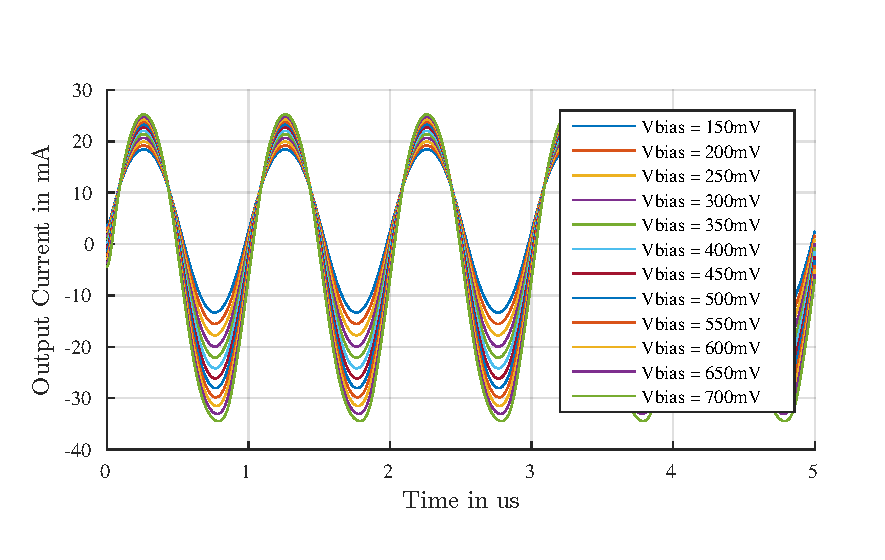
\includegraphics[scale=1]{Figures/Plots/Ov_Sine_Iout.pdf}
\caption{Plot of Output Current vs time for different Vbias}
\label{fig:SINE}
\end{figure}

Table.\ref{tab:SINE} gives a better picture of the sinusoidal plots shown above. The HD2 and HD3 values are less than 30 dBc. However, the HD3 seems to take a turn towards the worse with increase in $V_{bias}$. So for $V_{bias}$ values beyond 700mV, the output starts clipping at the trough of the current wave.

\begin{table} [H]
\centering
\begin{tabular}{@{}cccccc@{}}
\toprule
Vbias (mV)		& Iout Max(mA)		& Iout Min(mA)	 & Iout p2p(mA) & HD2 (dBc)	&HD3 (dBc) \\ \midrule
150				& 18.43	 			& -13.34		 & 31.77		& -37.14		& -48.17	\\
200				& 19.17 			& -15.55		 & 34.72		& -36.62		& -45.67	\\
250				& 19.93 			& -17.77		 & 37.7			& -35.65		& -43.65	\\
300				& 20.67 			& -19.97		 & 40.64		& -35.15		& -42.07	\\
350				& 21.38				& -22.12		 & 43.49		& -34.84		& -40.83	\\
400				& 22.04				& -24.19		 & 46.23		& -34.72		& -39.85	\\
450				& 22.66 			& -26.17		 & 48.83		& -34.8			& -39.01	\\
500				& 23.24				& -28.05		 & 51.29		& -35.08		& -38.24	\\
550				& 23.77	 			& -29.83		 & 53.6			& -35.54		& -37.42	\\
600				& 24.28 			& -31.51		 & 55.79		& -36.13		& -36.47	\\
650				& 24.76 			& -33.07		 & 57.83		& -36.61		& -35.24	\\
700 			& 25.24 			& -34.47		 & 59.71		& -36.44		& -33.61	\\
\bottomrule
\end{tabular}
\caption{Transient Parameters of the Overall System}
\label{tab:SINE}
\end{table}

Once the peak-to-peak value of current is obtained, we can use that to calculate the transconductance of the system for different $V_{bias}$ values. Transconductance is the ratio of output current to the input voltage. Since the output current is not symmetric around 0A, the the value half of peak-to-peak current is considered. That divided by the input voltage (100mV peak) would give us the required transconductance value. Figure.\ref{fig:GM} shows the plot of transconductance against $V_{bias}$. And it rightfully follows the behavior of the output current.

\begin{figure} [H]
\centering
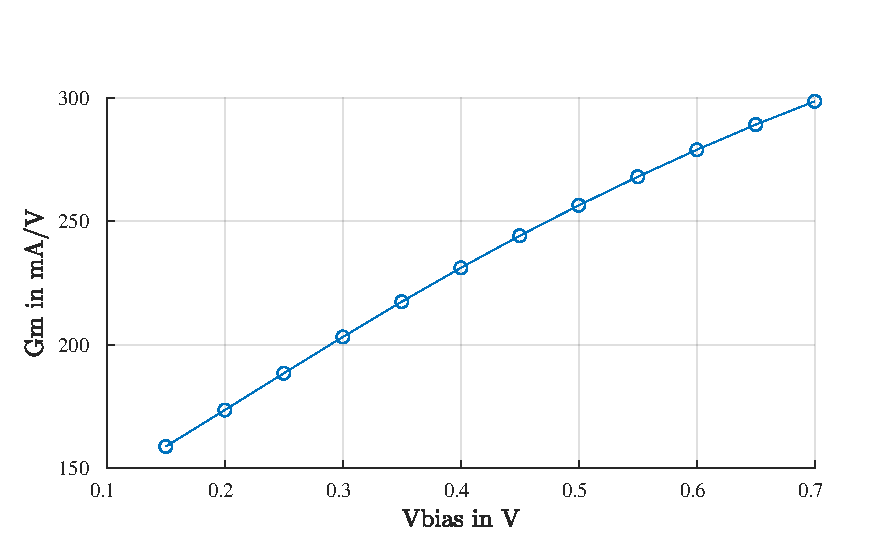
\includegraphics[scale=1]{Figures/Plots/Ov_Gm.pdf}
\caption{Plot of Gm vs Vbias}
\label{fig:GM}
\end{figure}

The transconductance value for each $V_{bias}$ used to plot the Figure.\ref{fig:GM} is tabulated in Table.\ref{tab:GM}.

\begin{table} [H]
\centering
\begin{tabular}{@{}cc@{}}
\toprule
Vbias (mV)			& Transconductance (mA/V)	\\ \midrule
150					& 158.8 \\
200					& 173.6 \\
250					& 188.5 \\
300					& 203.2 \\
350					& 217.5 \\
400					& 231.2 \\
450					& 244.2 \\
500					& 256.4 \\
550					& 268 \\
600					& 278.9 \\
650					& 289.1 \\
700 				& 298.5 \\
\bottomrule
\end{tabular}
\caption{Transconductance Gain of the Overall System}
\label{tab:GM}
\end{table}

Now, the second part of the transient analysis is performed with a square wave input. 
The slew rate for the rising edge and the falling edge is tabulated in the Table.\ref{tab:SLEW}. The slew rate is at a low value due to the fact that the OP AMP designed exhibits a very low slew rate.
 
\begin{table} [H]
\centering
\begin{tabular}{@{}ccc@{}}
\toprule
Vbias (mV)			& Slew Rate (Rising Edge)(V/us)			& Slew Rate (Falling Edge)(V/us)	 \\ \midrule
150					& 6.985	 					& -8.73					 \\
200					& 7.505 					& -9.779				 \\
250					& 8.042 					& -10.68				 \\
300					& 8.581 					& -11.34				 \\
350					& 9.095						& -11.66				 \\
400					& 9.561						& -11.7					 \\
450					& 9.954 					& -11.6					 \\
500					& 10.27						& -11.45				 \\
550					& 10.49	 					& -11.3					 \\
600					& 10.65 					& -11.14				 \\
650					& 10.76 					& -10.99				 \\
700 				& 10.82 					& -10.84				 \\
\bottomrule
\end{tabular}
\caption{Slew Rate of the Overall System}
\label{tab:SLEW}
\end{table}

\subsection{Noise Analysis}
The test bench to perform the noise analysis is same as the test bench used for AC analysis in Figure.(a). The input referred noise of the first stage is far more significant for the overall system than the second stage.

The Bode plot of the input referred noise for different values of $V_{bias}$ is shown in the Figure.\ref{fig:NOISE}. It is clear that the type of noise is 1/f noise or the Flicker noise. The magnitude of the input referred noise is very high for low frequencies and it reduces significantly in moderate and high frequencies when White noise starts to dominate.

\begin{figure} [H]
\centering
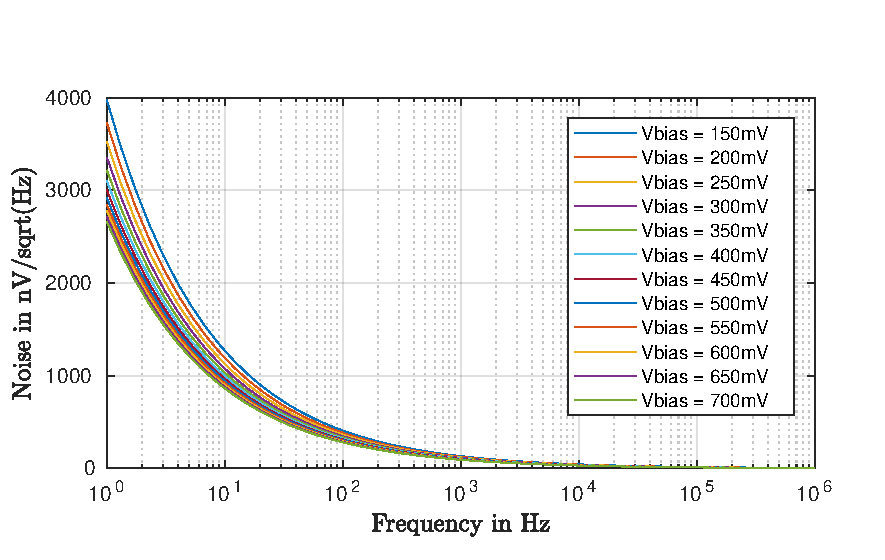
\includegraphics[scale=1]{Figures/Plots/Ov_Noise.pdf}
\caption{Plot of Input Referred Noise vs Frequency for different Vbias}
\label{fig:NOISE}
\end{figure}

The value of input referred noise at 1MHz for different $V_{bias}$ is tabulated in the Table.\ref{tab:NOISE}.

\begin{table} [H]
\centering
\begin{tabular}{@{}cc@{}}
\toprule
Vbias (mV)			& Input Referred Noise (nV/sqrt(Hz))	\\ \midrule
150					& 46.64 \\
200					& 43.93 \\
250					& 41.71 \\
300					& 39.91 \\
350					& 38.46 \\
400					& 37.29 \\
450					& 36.33 \\
500					& 35.52 \\
550					& 34.82 \\
600					& 34.21 \\
650					& 33.66 \\
700 				& 33.16 \\
\bottomrule
\end{tabular}
\caption{Input Referred Noise of the Overall System}
\label{tab:NOISE}
\end{table}


\section{Programmable Load}
Another way to make the overall system programmable is to have a programmable load. Having a Resistive load that varies would imply that the current flowing through the load is controlled. So, for the following analyses, the $V_{bias}$ is made constant and set a value of 425mV.

Table.\ref{tab:RL_AC_1} shows the variation of DC Gain, bandwidth, phase margin and transconductance with varying load. The gain hadly changes with the changing load. The variation in bandwidth is just 1.8MHz between the minimum and maximum load. The transconductance however, shows variation in a range that is expected.
 
\begin{table} [H]
\centering
\begin{tabular}{@{}ccccccc@{}}
\toprule
RL ($\Omega$)		& DC Gain(dB)		& Bandwidth(MHz)		& Phase Margin			& Transconductance(mA/V)\\ \midrule
35		& 22.2 		& 13.13		& 40.97		& 338.9		\\
40		& 22.22 	& 13.55		& 40.22		& 296.8		\\
45		& 22.25 	& 13.88		& 39.6		& 264		\\
50		& 22.28 	& 14.16		& 39.08		& 237.7		\\
55		& 22.3 		& 14.4		& 38.63		& 216.2		\\
60		& 22.32 	& 14.6		& 38.24		& 198.3		\\
65		& 22.34 	& 14.77		& 37.9	 	& 183.1		\\
70		& 22.35 	& 14.92		& 37.6		& 170		\\
\bottomrule
\end{tabular}
\caption{AC Parameters of the Overall System for a programmable load - 1}
\label{tab:RL_AC_1}
\end{table}

Table.\ref{tab:RL_AC_2} shows the tabulation of values for the parameters that are independent of the variation in load resistance.

\begin{table} [H]
\centering
\begin{tabular}{@{}cc@{}}
\toprule
Parameter							& Value		\\ \midrule
Input Impedance M($\Omega$)			& 3.436 	\\
Output Impedance ($\Omega$)			& 0.953 	\\
PSRR (VDD)(uA/V)					& 67.32 	\\
PSRR (VSS)(uA/V)					& 63.65 	\\
Input Referred Noise (nV/$\sqrt{Hz}$)	& 36.79		\\
\bottomrule
\end{tabular}
\caption{AC Parameters of the Overall System for a programmable load - 2}
\label{tab:RL_AC_2}
\end{table}

The transient analysis of the system with a programmable load shows a clear picture of how effective the system is. Since the bias voltage or the bias current doesn't change, the DC bias point at the output of the system remains unchanged. Therefore, we get a symmetrical waveform around 0A. The plot in Figure.\ref{fig:RL_SINE} shows the output current plot for different values of load resistance. 
\begin{figure} [H]
\centering
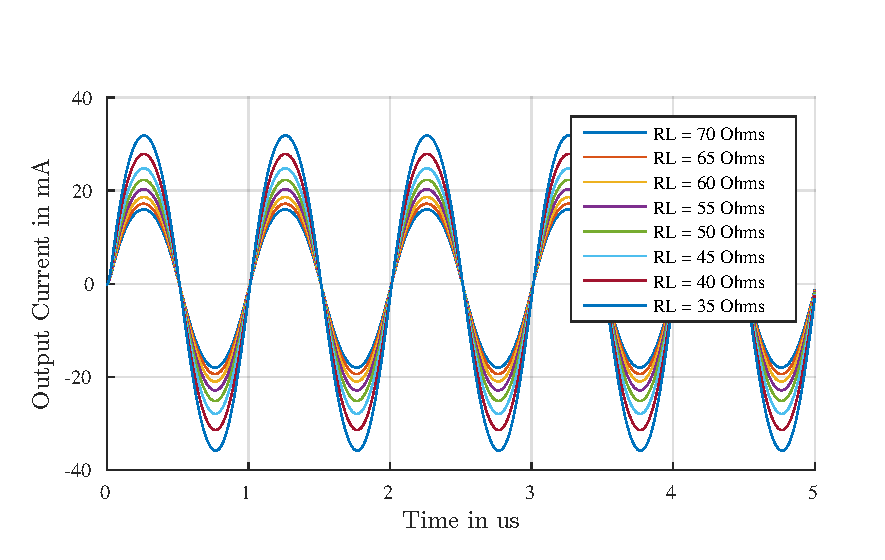
\includegraphics[scale=1]{Figures/Plots/Ov_Sine_RL.pdf}
\caption{Plot of Output Current vs Time for different RL}
\label{fig:RL_SINE}
\end{figure}
Table.\ref{tab:RL_trans_1} contains tabulation from the plot in Figure.\ref{fig:RL_SINE}. Output current is the most significant parameter that gets affected by a variable load.
\begin{table} [H]
\centering
\begin{tabular}{@{}cccc@{}}
\toprule
RL ($\Omega$)			& Iout(max)(mA)		& Iout(min)(mA)		& Iout(p2p)(mA) \\ \midrule
35					& 31.89 			& -35.89			& 67.77			\\
40					& 27.92 			& -31.44			& 59.36			\\
45					& 24.83 			& -27.97			& 52.8			\\
50					& 22.36 			& -25.19			& 47.55			\\
55					& 20.33 			& -22.91			& 43.24			\\
60					& 18.65 			& -21.01			& 39.65			\\
65					& 17.22 			& -19.4				& 36.61 		\\
70					& 15.99 			& -18.02			& 34.01			\\
\bottomrule
\end{tabular}
\caption{Maximum and Minimum Output Currents for a programmable load}
\label{tab:RL_trans_1}
\end{table}

Table.\ref{tab:RL_trans_2} shows the values of the parameters that are constant with a varying load. HD2 and HD3 are less than -30dBc.
\begin{table} [H]
\centering
\begin{tabular}{@{}cc@{}}
\toprule
Parameter							& Value		\\ \midrule
HD2 (dBc)							& -34.6 			\\
HD3 (dBc)							& -39.4 			\\
Slew Rate (Rising Edge)(V/us)		& 10.28 			\\
Slew Rate (Falling Edge)(V/us)		& -10.45 			\\
\bottomrule
\end{tabular}
\caption{Transient Parameters of the Overall System for a programmable load}
\label{tab:RL_trans_2}
\end{table}
And finally, we have the plot of transconductance versus the load resistance as shown in Figure.\ref{fig:RL_Gm}
\begin{figure} [H]
\centering
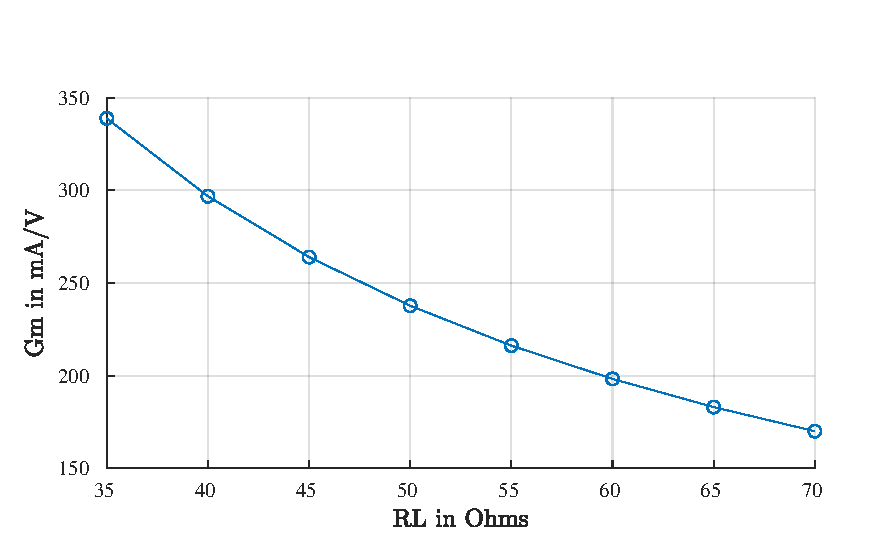
\includegraphics[scale=1]{Figures/Plots/Ov_Gm_RL.pdf}
\caption{Plot of Transconductance vs RL}
\label{fig:RL_Gm}
\end{figure}

\section{Summary of Results}



\chapter{Corner Simulations}
Corner analysis is performed to simulate the circuit's performance against a set of parameters belonging to extreme manufacturing variations. Corner simulations are performed to verify that the circuit works at all possible conditions of process, supply voltage and temperature. An analog circuit designs that perform sufficiently well across these corners are to be considered a robust design.

\section{Process Variation}

Process variation is the naturally occurring variation in the attributes of transistors (length, widths, oxide thickness) when ICs are fabricated. In general there are 5 corners - tt, ff, ss, fs, sf. Transistors can be typical, fast or slow. The first letter indicates the PMOS and the second letter indicates the NMOS. However, as part of XT018 technology, the corners are termed as - tm, wp, ws, wo, wz. The meaning and their translation to the general conventions are described in Table.\ref{tab:Process_Corners}. The process corners of Capacitors and Resistors too follow a similar naming convention but with only 3 corners - tm (typical), wp(minimum), ws(maximum).

\begin{table} [H]
\centering
\begin{tabular}{@{}ccc@{}}
\toprule
Corner	& Expansion						& Translation	\\ \midrule
tm		& Typical Mean Condition 		& tt			\\
wp		& Worst Case Power Condition	& ff			\\
ws		& Worst Case Speed Condition 	& ss			\\
wo		& Worst Case One Condition 		& fs			\\
wz		& Worst Case Zero Condition 	& sf			\\
\bottomrule
\end{tabular}
\caption{Different Corners for MOS Transistors in XT018 Technology}
\label{tab:Process_Corners}
\end{table}

A total of 45 corners are simulated for 2 values of $V_{bias}$ - 150mV and 700mV. The results are presented in the subsequent sections.

\subsubsection{Lowest $V_{bias}$}
At the lowest $V_{bias}$, the mean values of all parameters satisfy the requirement. In the worst corner, the positive peak of the current goes below 10mA but the negative peak is still under -15mA. So the current swing is decreased. 
\begin{figure} [H]
\centering
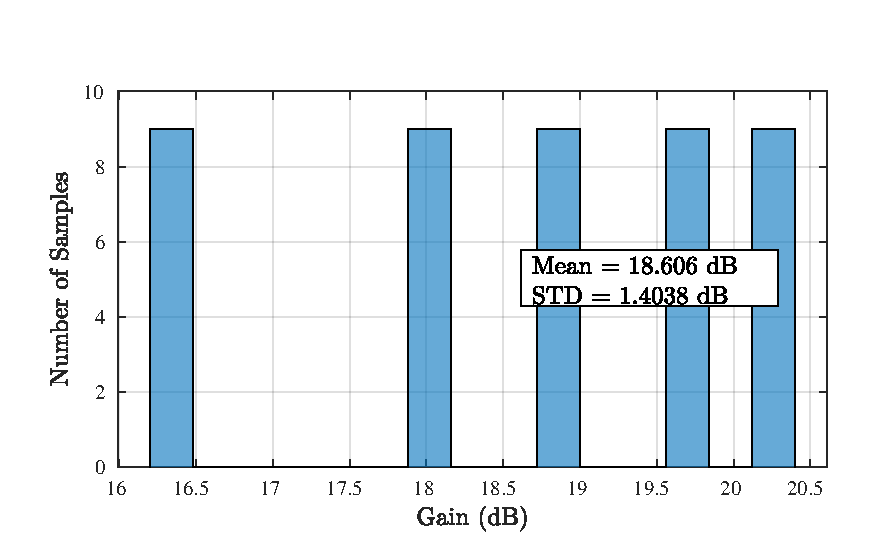
\includegraphics[scale=1]{Figures/Corners/Overall/Proc_Min/PDFs/Proc_Min_gain.pdf}
\caption{Histogram of System Gain due to Process Variation at $V_{bias}$=150mV}
\end{figure}

\begin{figure} [H]
\centering
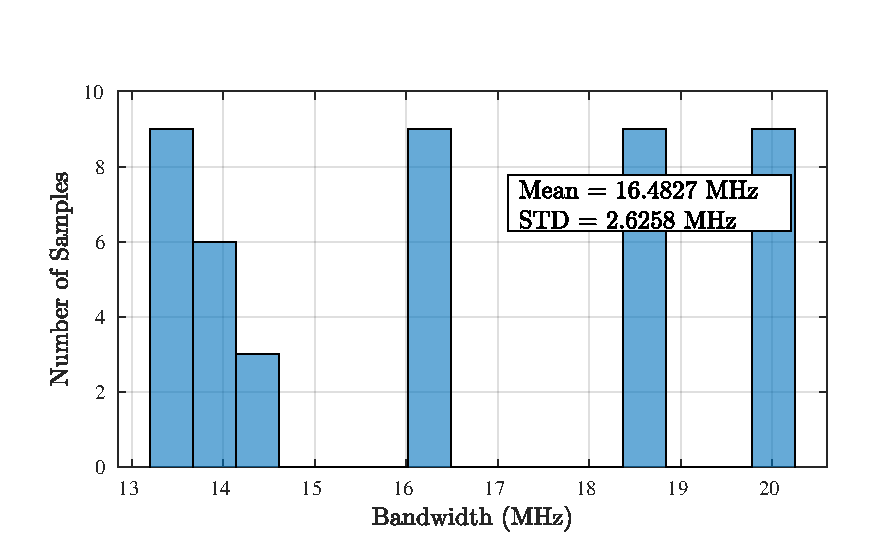
\includegraphics[scale=1]{Figures/Corners/Overall/Proc_Min/PDFs/Proc_Min_bw.pdf}
\caption{Histogram of System Bandwidth due to Process Variation at $V_{bias}$=150mV}
\end{figure}

\begin{figure} [H]
\centering
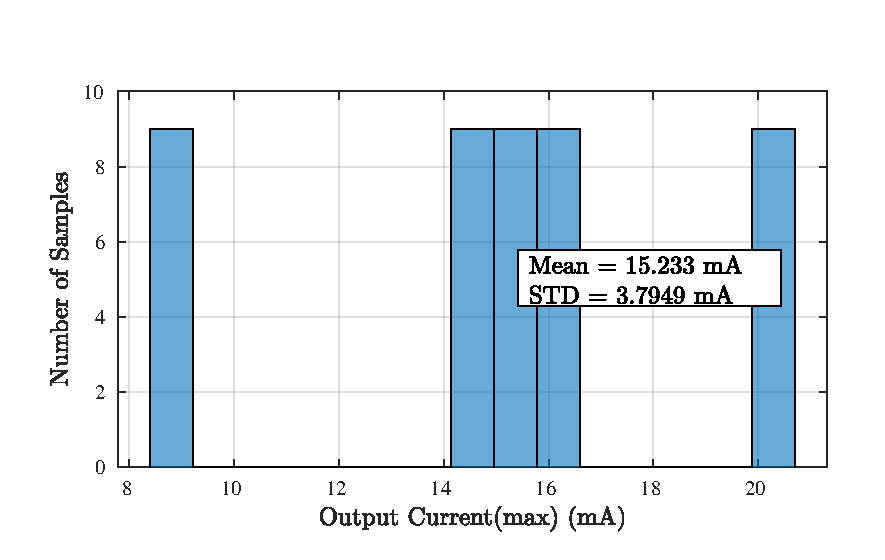
\includegraphics[scale=1]{Figures/Corners/Overall/Proc_Min/PDFs/Proc_Min_imax.pdf}
\caption{Histogram of Maximum Output Current due to Process Variation at $V_{bias}$=150mV}
\end{figure}

\begin{figure} [H]
\centering
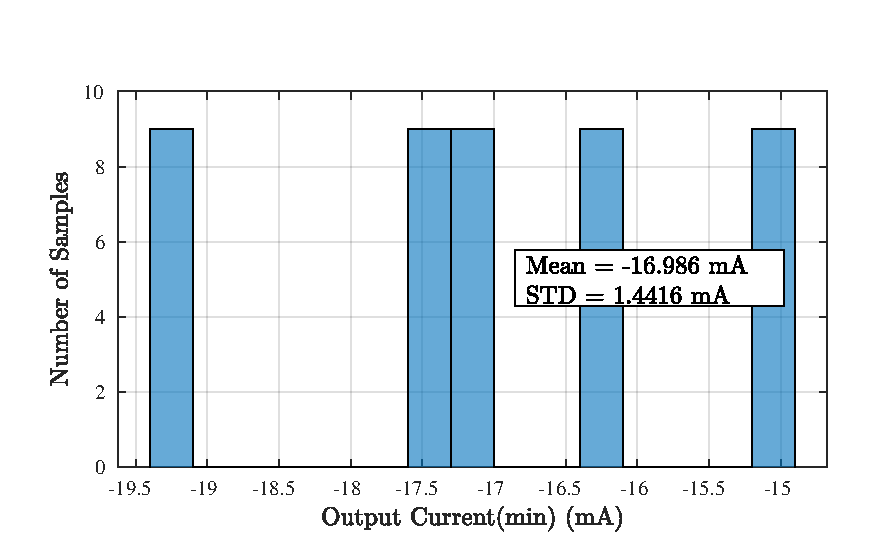
\includegraphics[scale=1]{Figures/Corners/Overall/Proc_Min/PDFs/Proc_Min_imin.pdf}
\caption{Histogram of Minimum Output Current due to Process Variation at $V_{bias}$=150mV}
\end{figure}

\subsubsection{Highest $V_{bias}$}
At the highest $V_{bias}$, the mean values of the parameters meet the requirements. At the worst corner, the positive peak of the output current slips to 20mA but the peak to peak current is still under the requirement. Since the spread is smaller for all parameters, none of them fail to meet the requirements.
\begin{figure} [H]
\centering
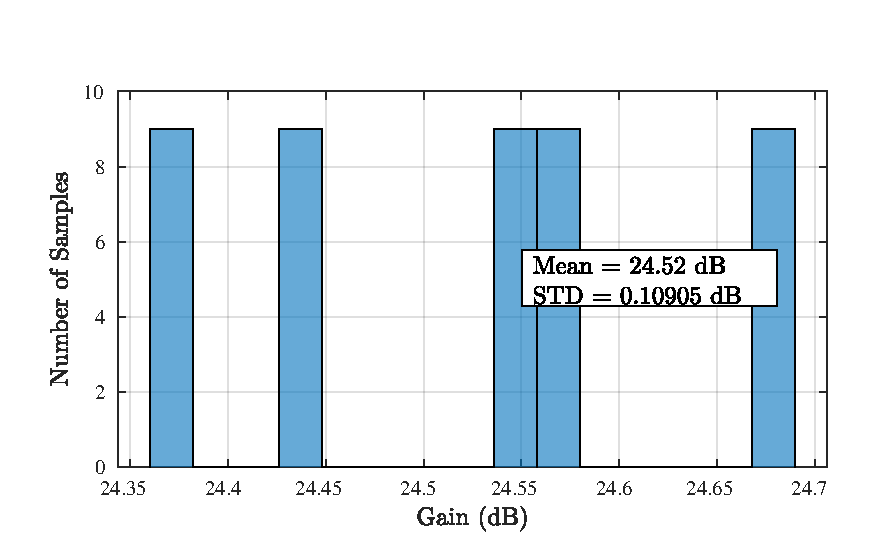
\includegraphics[scale=1]{Figures/Corners/Overall/Proc_Max/PDFs/Proc_Max_gain.pdf}
\caption{Histogram of System Gain due to Process Variation at $V_{bias}$=700mV}
\end{figure}

\begin{figure} [H]
\centering
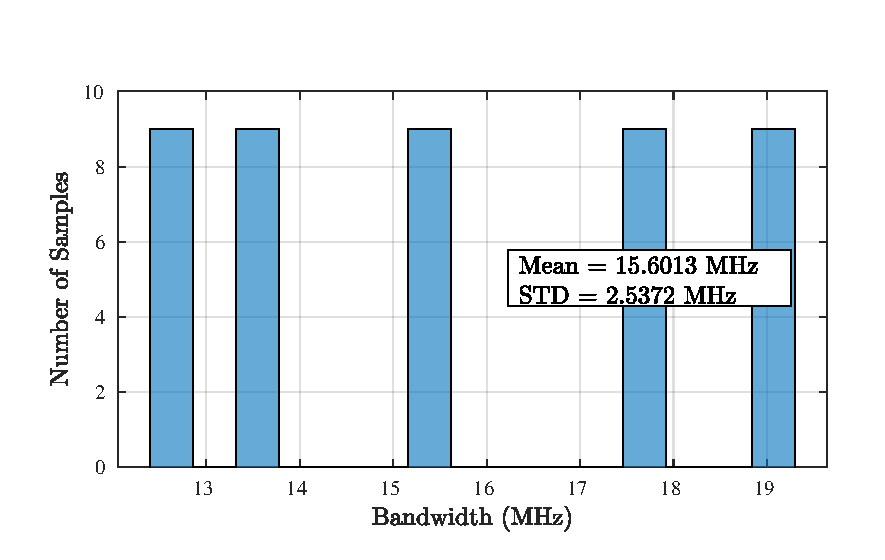
\includegraphics[scale=1]{Figures/Corners/Overall/Proc_Max/PDFs/Proc_Max_bw.pdf}
\caption{Histogram of System Bandwidth due to Process Variation at $V_{bias}$=700mV}
\end{figure}

\begin{figure} [H]
\centering
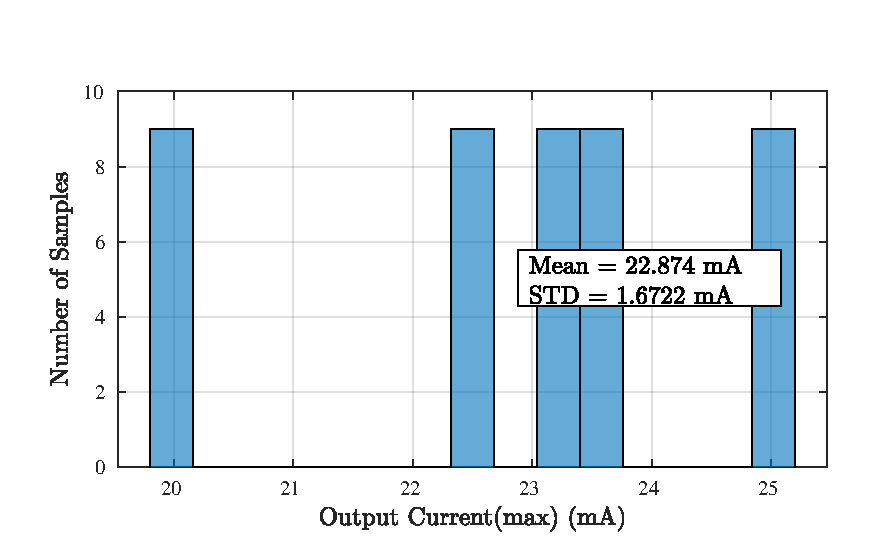
\includegraphics[scale=1]{Figures/Corners/Overall/Proc_Max/PDFs/Proc_Max_imax.pdf}
\caption{Histogram of Maximum Output Current due to Process Variation at $V_{bias}$=700mV}
\end{figure}

\begin{figure} [H]
\centering
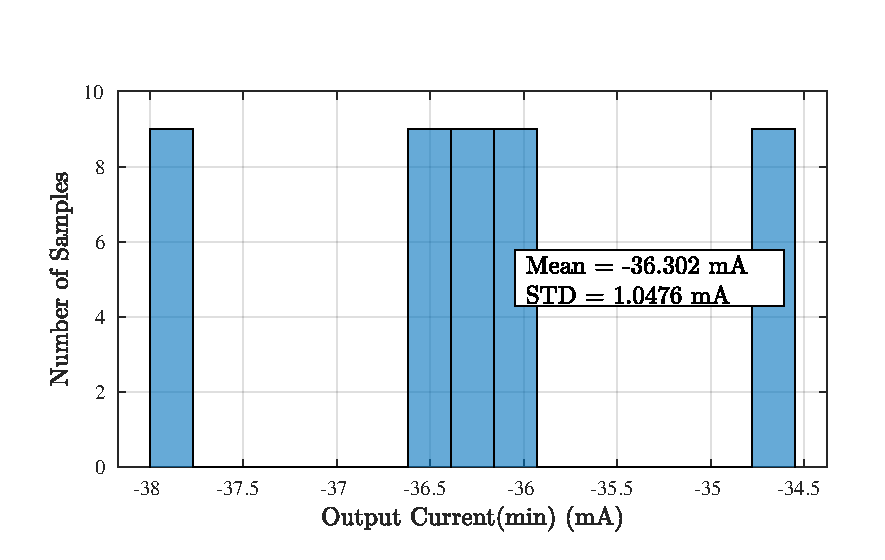
\includegraphics[scale=1]{Figures/Corners/Overall/Proc_Max/PDFs/Proc_Max_imin.pdf}
\caption{Histogram of Minimum Output Current due to Process Variation at $V_{bias}$=700mV}
\end{figure}
\vfill
\clearpage

\section{Process and Supply Variation}

In addition to process variation, the system responds to power supply variations too. 3 different corners are obtained by evaluating the power supply with $\pm$10\% from the nominal value. Therefore, we get 3 corners for $V_{DD}$ - 2.5V, 2.25V, 2.75V and 3 corners for $V_{SS}$ - -2.5V, -2.25V, -2.75V. The total number of corners in this case are 405. And the results are discussed in the subsequent sections.

\subsubsection{Lowest $V_{bias}$}
Additional variation in power supply increases the spread in the histogram with samples for gain at 12dB and as high as 21dB. The mean values of all parameters are well within their specified range. But the positive peak output current value drops to a negative value for the worst case. The negative output current for the same case is at -10mA which makes the peak to peak current of 9mA, which is little far from what is required.

\begin{figure} [H]
\centering
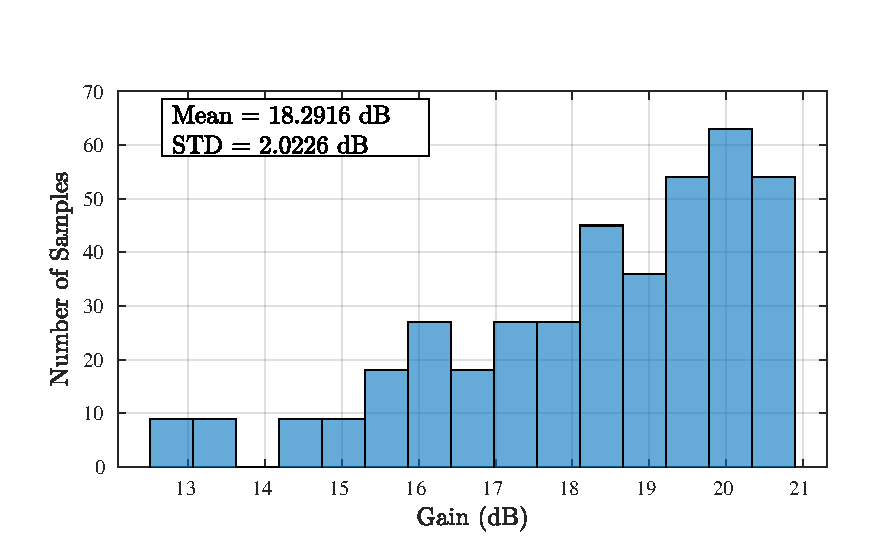
\includegraphics[scale=1]{Figures/Corners/Overall/PV_Min/PDFs/PV_Min_gain.pdf}
\caption{Histogram of System Gain due to Process and Supply Variation at $V_{bias}$=150mV}
\end{figure}

\begin{figure} [H]
\centering
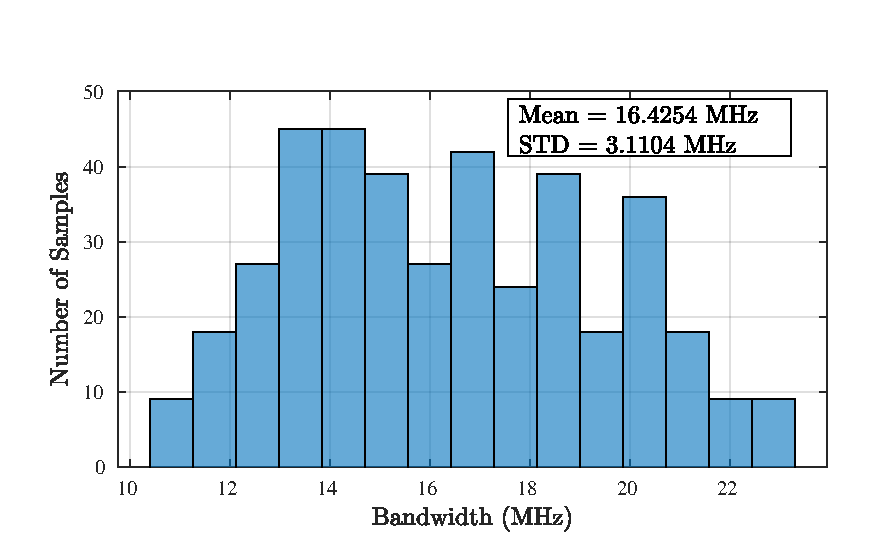
\includegraphics[scale=1]{Figures/Corners/Overall/PV_Min/PDFs/PV_Min_bw.pdf}
\caption{Histogram of System Bandwidth due to Process and Supply Variation at $V_{bias}$=150mV}
\end{figure}

\begin{figure} [H]
\centering
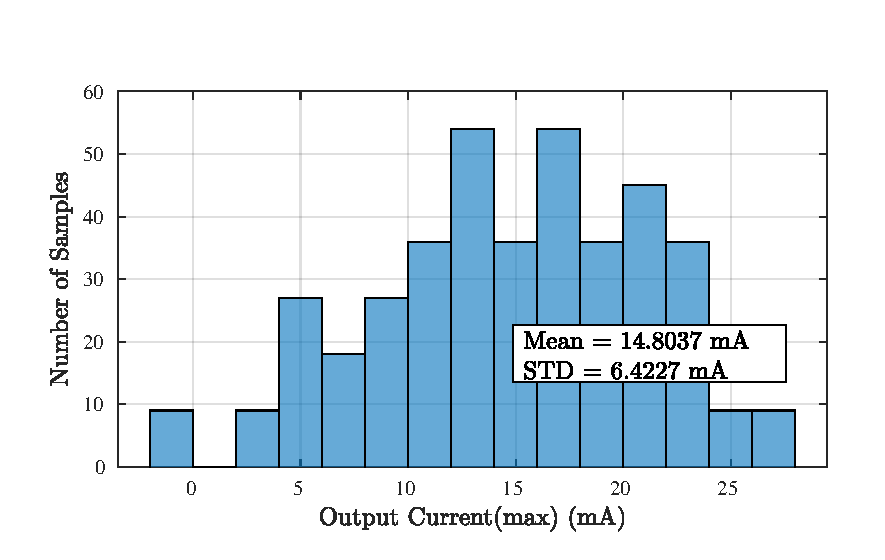
\includegraphics[scale=1]{Figures/Corners/Overall/PV_Min/PDFs/PV_Min_imax.pdf}
\caption{Histogram of Maximum Output Current due to Process and Supply Variation at $V_{bias}$=150mV}
\end{figure}

\begin{figure} [H]
\centering
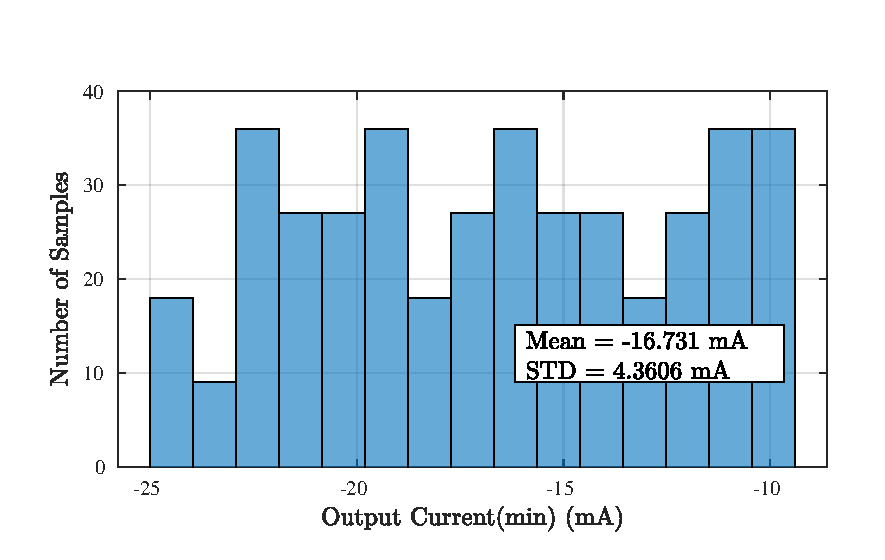
\includegraphics[scale=1]{Figures/Corners/Overall/PV_Min/PDFs/PV_Min_imin.pdf}
\caption{Histogram of Minimum Output Current due to Process and Supply Variation at $V_{bias}$=150mV}
\end{figure}

\begin{figure} [H]
\centering
\includegraphics[scale=1]{Figures/Corners/Overall/PV_Min/PDFs/PV_Min_gm.pdf}
\caption{Histogram of Transconductance due to Process and Supply Variation at $V_{bias}$=150mV}
\end{figure}

\subsubsection{Highest $V_{bias}$}
The spread is wide for the bandwidth but even in the worst corner, the bandwidth is above 10MHz and the mean value being 15MHz. The spread for the gain is comparatively smaller with the mean value being 24.5dB and the standard deviation of 0.62dB. The slow corners are once again the worst case corners with the positive current peak dropping 16mA from a mean value of 22mA.
\begin{figure} [H]
\centering
\includegraphics[scale=1]{Figures/Corners/Overall/PV_Max/PDFs/PV_Max_gain.pdf}
\caption{Histogram of System Gain due to Process and Supply Variation at $V_{bias}$=700mV}
\end{figure}

\begin{figure} [H]
\centering
\includegraphics[scale=1]{Figures/Corners/Overall/PV_Max/PDFs/PV_Max_bw.pdf}
\caption{Histogram of System Bandwidth due to Process and Supply Variation at $V_{bias}$=700mV}
\end{figure}

\begin{figure} [H]
\centering
\includegraphics[scale=1]{Figures/Corners/Overall/PV_Max/PDFs/PV_Max_imax.pdf}
\caption{Histogram of Maximum Output Current due to Process and Supply Variation at $V_{bias}$=700mV}
\end{figure}

\begin{figure} [H]
\centering
\includegraphics[scale=1]{Figures/Corners/Overall/PV_Max/PDFs/PV_Max_imin.pdf}
\caption{Histogram of Minimum Output Current due to Process and Supply Variation at $V_{bias}$=700mV}
\end{figure}

\begin{figure} [H]
\centering
\includegraphics[scale=1]{Figures/Corners/Overall/PV_Max/PDFs/PV_Max_gm.pdf}
\caption{Histogram of Transconductance due to Process and Supply Variation at $V_{bias}$=700mV}
\end{figure}

\begin{figure} [H]
\centering
\includegraphics[scale=1]{Figures/Corners/Overall/PV_Max/PDFs/PV_Max_irn.pdf}
\caption{Histogram of Input Referred Noise due to Process and Supply Variation at $V_{bias}$=400mV}
\end{figure}

\section{Process, Voltage and Temperature (PVT) variation}

Another possible variation is seen in the temperature parameter. The PVT corner simulations are performed at the following corners:
\begin{itemize}
\item All Process corners mentioned in Section 4.6.1.
\item $\pm$10\% variations of $V_{DD}$ i.e., 2.5V, 2.25V, 2.75V and $V_{SS}$ i.e., -2.5V, -2.25V, -2.75V.
\item Three temperature conditions: -25$^0$C, 25$^0$C and 80$^0$C.
\end{itemize}

Therefore, there are 1215 corners in total. The results are provided in the subsequent sections.

\subsubsection{Lowest $V_{bias}$}
With all the variations included, it is observed that the worst case is caused by the supply variations and the temperature variation has lower effect than the suuply variation. The worst case corners are still affected by the voltage but with normal spread. The mean gain is 18.3dB with a standard deviation of 2.1dB. The bandwidth too has a wide spread like the gain histogram and at the worst case, it falls just a tad below 10MHz with the mean and standard deviation being 16MHz and 4MHz respectively. The HD2 and HD3 values are less than -30dBc even for worst cases. The PSRR however, at worst case, goes to a value beyond 160$\mu$A/V

\begin{figure} [H]
\centering
\includegraphics[scale=1]{Figures/Corners/Overall/PVT_Min/PDFs/PVT_Min_gain.pdf}
\caption{Histogram of System Gain due to PVT Variation at $V_{bias}$=150mV}
\end{figure}

\begin{figure} [H]
\centering
\includegraphics[scale=1]{Figures/Corners/Overall/PVT_Min/PDFs/PVT_Min_bw.pdf}
\caption{Histogram of System Bandwidth due to PVT Variation at $V_{bias}$=150mV}
\end{figure}

\begin{figure} [H]
\centering
\includegraphics[scale=1]{Figures/Corners/Overall/PVT_Min/PDFs/PVT_Min_imax.pdf}
\caption{Histogram of Maximum Output Current due to PVT Variation at $V_{bias}$=150mV}
\end{figure}

\begin{figure} [H]
\centering
\includegraphics[scale=1]{Figures/Corners/Overall/PVT_Min/PDFs/PVT_Min_imin.pdf}
\caption{Histogram of Minimum Output Current due to PVT Variation at $V_{bias}$=150mV}
\end{figure}

\begin{figure} [H]
\centering
\includegraphics[scale=1]{Figures/Corners/Overall/PVT_Min/PDFs/PVT_Min_gm.pdf}
\caption{Histogram of Transconductance due to PVT Variation at $V_{bias}$=150mV}
\end{figure}

\begin{figure} [H]
\centering
\includegraphics[scale=1]{Figures/Corners/Overall/PVT_Min/PDFs/PVT_Min_hd2.pdf}
\caption{Histogram of HD2 due to PVT Variation at $V_{bias}$=150mV}
\end{figure}

\begin{figure} [H]
\centering
\includegraphics[scale=1]{Figures/Corners/Overall/PVT_Min/PDFs/PVT_Min_hd3.pdf}
\caption{Histogram of HD3 due to PVT at $V_{bias}$=150mV}
\end{figure}

\begin{figure} [H]
\centering
\includegraphics[scale=1]{Figures/Corners/Overall/PVT_Min/PDFs/PVT_Min_irn.pdf}
\caption{Histogram of Input Referred Noise due to PVT Variation at $V_{bias}$=150mV}
\end{figure}

\begin{figure} [H]
\centering
\includegraphics[scale=1]{Figures/Corners/Overall/PVT_Min/PDFs/PVT_Min_zin.pdf}
\caption{Histogram of Input Impedance due to PVT Variation at $V_{bias}$=150mV}
\end{figure}

\begin{figure} [H]
\centering
\includegraphics[scale=1]{Figures/Corners/Overall/PVT_Min/PDFs/PVT_Min_zout.pdf}
\caption{Histogram of Output Impedance due to PVT Variation at $V_{bias}$=150mV}
\end{figure}

\begin{figure} [H]
\centering
\includegraphics[scale=1]{Figures/Corners/Overall/PVT_Min/PDFs/PVT_Min_psrrp.pdf}
\caption{Histogram of PSRR($V_{DD}$) due to PVT Variation at $V_{bias}$=150mV}
\end{figure}

\begin{figure} [H]
\centering
\includegraphics[scale=1]{Figures/Corners/Overall/PVT_Min/PDFs/PVT_Min_psrrn.pdf}
\caption{Histogram of PSRR($V_{SS}$) due to PVT Variation at $V_{bias}$=150mV}
\end{figure}

\subsubsection{Highest $V_{bias}$}
For the highest $V_{bias}$, the mean gain is around 24dB with a standard deviation of 0.7dB. The spread for the gain histogram is comparatively narrower in comparison to the lowest $V_{bias}$. Once again the bandwidth just falls short of 10MHz for the worst case corner. The mean values of the currents are 23mA and -35mA. But at the worst case corner, the peak-to-peak current is as low as 40mA. The mean values of HD2 and HD3 are below -30dBc but they rise above the -30dBc mark for slow corners. The input referred noise spread is much smaller for highest $V_{bias}$ with a mean value of 32.985nV/$\sqrt{Hz}$.

\begin{figure} [H]
\centering
\includegraphics[scale=1]{Figures/Corners/Overall/PVT_Max/PDFs/PVT_Max_gain.pdf}
\caption{Histogram of System Gain due to PVT Variation at $V_{bias}$=700mV}
\end{figure}

\begin{figure} [H]
\centering
\includegraphics[scale=1]{Figures/Corners/Overall/PVT_Max/PDFs/PVT_Max_bw.pdf}
\caption{Histogram of System Bandwidth due to PVT Variation at $V_{bias}$=700mV}
\end{figure}

\begin{figure} [H]
\centering
\includegraphics[scale=1]{Figures/Corners/Overall/PVT_Max/PDFs/PVT_Max_imax.pdf}
\caption{Histogram of Maximum Output Current due to PVT Variation at $V_{bias}$=700mV}
\end{figure}

\begin{figure} [H]
\centering
\includegraphics[scale=1]{Figures/Corners/Overall/PVT_Max/PDFs/PVT_Max_imin.pdf}
\caption{Histogram of Minimum Output Current due to PVT Variation at $V_{bias}$=700mV}
\end{figure}

\begin{figure} [H]
\centering
\includegraphics[scale=1]{Figures/Corners/Overall/PVT_Max/PDFs/PVT_Max_gm.pdf}
\caption{Histogram of Transconductance due to PVT Variation at $V_{bias}$=700mV}
\end{figure}

\begin{figure} [H]
\centering
\includegraphics[scale=1]{Figures/Corners/Overall/PVT_Max/PDFs/PVT_Max_hd2.pdf}
\caption{Histogram of HD2 due to PVT Variation at $V_{bias}$=700mV}
\end{figure}

\begin{figure} [H]
\centering
\includegraphics[scale=1]{Figures/Corners/Overall/PVT_Max/PDFs/PVT_Max_hd3.pdf}
\caption{Histogram of HD3 due to PVT Variation at $V_{bias}$=700mV}
\end{figure}

\begin{figure} [H]
\centering
\includegraphics[scale=1]{Figures/Corners/Overall/PVT_Max/PDFs/PVT_Max_irn.pdf}
\caption{Histogram of Input Referred Noise due to PVT Variation at $V_{bias}$=400mV}
\end{figure}

\begin{figure} [H]
\centering
\includegraphics[scale=1]{Figures/Corners/Overall/PVT_Max/PDFs/PVT_Max_zin.pdf}
\caption{Histogram of Input Impedance due to PVT Variation at $V_{bias}$=700mV}
\end{figure}

\begin{figure} [H]
\centering
\includegraphics[scale=1]{Figures/Corners/Overall/PVT_Max/PDFs/PVT_Max_zout.pdf}
\caption{Histogram of Output Impedance due to Process and Supply Variation at $V_{bias}$=700mV}
\end{figure}

\begin{figure} [H]
\centering
\includegraphics[scale=1]{Figures/Corners/Overall/PVT_Max/PDFs/PVT_Max_psrrp.pdf}
\caption{Histogram of PSRR($V_{DD}$) due to PVT Variation at $V_{bias}$=700mV}
\end{figure}

\begin{figure} [H]
\centering
\includegraphics[scale=1]{Figures/Corners/Overall/PVT_Max/PDFs/PVT_Max_psrrn.pdf}
\caption{Histogram of PSRR($V_{SS}$) due to PVT Variation at $V_{bias}$=700mV}
\end{figure}

\vfill
\clearpage
\section{Summary of PVT Corner Analysis}
The summary of all PVT corners of the lowest and highest $V_{bias}$ is presented in this section. As seen in the previous sections, the current is worst at lowest $V_{bias}$, with a value of -1.62mA.
The worst case open loop gain of the OTA is 12dB for the lowest $V_{bias}$. The mean values of all the parameters are very close to the typical or nominal case.
\begin{table} [H]
\centering
\begin{tabular}{@{}cccc@{}}
\toprule
Parameter					& Min			& Max 				& Mean			\\ \midrule
Transconductance Gain(Gm)	& 81 mA/V		& 241 mA/V 			& 158.2 mA/V	\\
Output Current(+)			& -1.626 mA		& 28.01 mA			& 14.79 mA		\\
Output Current(-)			& -28.41 mA		& -7.123 mA			& -16.84 mA		\\
Bandwidth					& 8.858 MHz		& 28.46 MHz			& 16.7 MHz		\\
Input Referred Noise		& 36.62 nV/$\sqrt{Hz}$	& 75.85 nV/$\sqrt{Hz}$	& 48.96 nV/$\sqrt{Hz}$\\
Input Impedance				& 3.241 M$\Omega$	& 3.352 M$\Omega$ & 3.388 M$\Omega$	\\
Output Impedance			& 0.418$\Omega$		& 2.207$\Omega$	& 0.968$\Omega$	\\
HD2							& -63.12 dBc		& -31.12 dBc	& -41.2 dBc		\\
HD3							& -78.03 dBc		& -39.28 dBc	& -51.6 dBc		\\
Open Loop Voltage Gain		& 12.3 dB			& 22.51 dB		& 18.3 dB		\\
PSRR						& 61.04 $\mu$A/V	& 205.1 $\mu$A/V & 96.14 $\mu$A/V \\
\bottomrule
\end{tabular}
\caption{PVT Corners for $V_{bias}$ = 150mV}
\label{tab:PVT_150}
\end{table}

\begin{table} [H]
\centering
\begin{tabular}{@{}cccc@{}}
\toprule
Parameter					& Min				& Max 			& Mean			\\ \midrule
Transconductance Gain(Gm)	& 241.7 mA/V		& 319.3 mA/V 	& 290.49 mA/V	\\
Output Current(+)			& 13.6 mA			& 29.99 mA		& 22.96 mA		\\
Output Current(-)			& -44.21 mA			& -23.01 mA		& -35.13 mA		\\
Bandwidth					& 8.235 MHz			& 27.15 MHz		& 15.8 MHz		\\
Input Referred Noise		& 27.62 nV/$\sqrt{Hz}$	& 38.52 nV/$\sqrt{Hz}$	& 32.985 nV/$\sqrt{Hz}$\\
Input Impedance				& 3.327 M$\Omega$	& 3.675 M$\Omega$ & 3.49 M$\Omega$ \\
Output Impedance			& 0.427$\Omega$		& 2.287$\Omega$	& 0.996$\Omega$	\\
HD2							& -48.93 dBc		& -18.36 dBc	& -31.72 dBc	\\
HD3							& -39.28 dBc		& -22.5 dBc		& -30.94 dBc	\\
Open Loop Voltage Gain		& 22.5 dB			& 26.14 dB		& 24.52 dB		\\
PSRR						& 40.76 $\mu$A/V	& 64.63 $\mu$A/V & 51.3 $\mu$A/V \\
\bottomrule
\end{tabular}
\caption{PVT Corners for $V_{bias}$ = 700mV}
\label{tab:PVT_700}
\end{table}


\chapter{Conclusion}
A high output current transconductance amplifier was designed and implemented using the XT018 SOI technology from XFAB. The amplifier consists of two stages - 
\begin{enumerate}
\item A programmable operational transconductance amplifier that is based on conventional current mirror technique. The output voltage is controlled by an external voltage that indrectly controls the bias current.
\item An operational amplifier based on the two-stage Miller compensation technique is used as a voltage buffer. This stage produces high currents due the bulky dimensions of the common source amplifier.
\end{enumerate}
The range of currents produced by this system is from $\pm$15mA to $\pm$30mA. The programmable parameter - the external bias voltage is swept from 150mV to 700mV and the output is measured across a 50$\Omega$ load resistor. For this setup though, the DC bias voltage at the output of the amplifier is not a constant as the variable parameter is the bias current. However, the design is tweaked in such a way that the variation is minimal. Another set of result is provided with a fixed external voltage, a fixed bias current but a variable load resistor. In this case, the same range of output current is obtained for an external bias voltage of 450mV and the load varying from 35$\Omega$ to 70$\Omega$. The advantage of this setup in comparison to the previous setup is the fact that the DC Bias voltage at the output does not vary with variation in the programmable parameter. The operating bandwidth for both sets of results is around 14MHz and the 2nd and 3rd harmonic distortion are less than -30dB with respect to the carrier frequency.

\section{Summary of Results}

\begin{table} [H]
\centering
\begin{tabular}{@{}cccc@{}}
\toprule
Parameter						& Value/Specification			& Programmable Voltage			& Programmable Resistor	\\ \midrule
Circuit Design					& Programmability				& External Votlage $V_{bias}$	& Load Resistor $R_L$	\\
Transconductance Gain(Gm)		& 75 .. 140 mA/V				& 158.8 .. 298.5 mA/V			& 170 .. 338.9 mA/V		\\
Linear Input Voltage Range		& $\pm$200 mV					& $\pm$100 mV					& $\pm$100 mV			\\
Output Current Range			& $\pm$15 mA 					& +18 mA .. -13 mA				& +15 mA .. -18 mA		\\
Bandwidth						& 10 MHz						& 13.8 MHz						& 13.13 MHz				\\
Slew Rate						& $\pm$900 V/$\mu$s				& $\pm$10.82 V/$\mu$s			& $\pm$10.28 V/$\mu$s	\\
Rise/Fall time					& 4.4 ns						& 22.7 ns						& 23.5 ns				\\
Input Referred Noise			& 3 nV/$\sqrt{Hz}$ @few KHz		& 46.64 nV/$\sqrt{Hz}$ @1MHz	& 36.79 nV/$\sqrt{Hz}$ @1MHz\\
Input Impedance					& 0.5 M$\Omega$					& 3.394 M$\Omega$				& 3.436 M$\Omega$		\\
Output Impedance				& 55 K$\Omega$					& 0.9415 $\Omega$				& 0.953 $\Omega$		\\
HD2								& Less than -75 dBc				& -34.72 dBc					& -34.6 dBc				\\
HD3								& Less than -80 dBc				& -33.61 dBc					& -39.4 dBc				\\
Open Loop Voltage Gain			& Not less than+5 V/V			& 8.41 V/V						& 12.9 V/V				\\
PSRR							& $\pm$20 $\mu$A/V				& 97.76 $\mu$A/V				& 67.32 $\mu$A/V		\\
\bottomrule
\end{tabular}
\caption{Specification vs Results}
\label{tab:Results}
\end{table}

Table.\ref{tab:Results} summarizes the results of the overall system and compares it with the actual specificaitons. First remark here is about linear input voltage range. Due to varying bias currents of the OTA, the gain keeps varying too. And to avoid saturation, the gain must be low. But OTAs in general have very high gain than a conventional OP AMP. So for this reason, to avoid saturation at the output, the input voltage range is reduced to 100mV instead of 200mV. And consequently, the transconductance parameter is double of what it should have been. The other parameters are picked from the commercial OTA OPA860 (citation) hence it is bit tricky to reach all of those specifications considering that the topology, technology and the power supply requirements are completely different. The key thing here is to note the output impedance requirements. Ideally current sources have infinite output impedance. But practially speaking, for a high current amplifier, with an output buffer, a high impedance at the output node is impractical to achieve.

\section{Outlook}

The amplifier designed has been simulated at all corners. The OTA can be used to test the Closed loop NDCCT. There is no second thought that there is room for improvement and further optimization of the amplifier to better meet the specifications. But this needs more research, and implementation of blocks like slew rate enhancer, current feedback amplifier, and possibly an emitter follower to amplify the current further if necessary.

\begin{appendices}
\chapter{Appendix}

\end{appendices}

\printglossary[type=acronym, title=Acronyms, toctitle=Acronyms]

\bibliography{ota}
\bibliographystyle{ieeetr}
\end{document}